% Autor: Betti Oesterholz
% erstellt: 05.03.2008
% main document for Fib V1.0
%
% This is the main document of the english Fib documentationen.
% It is a short version of the german documentation.
%
% Copyright (c) 2008 Betti Oesterholz
%
% Permission is granted to copy, distribute and/or modify this document
% under the terms of the GNU Free Documentation License, Version 1.2 or
% any later version published by the Free Software Foundation;
% with no Invariant Sections, no Front-Cover Texts, and no Back-Cover Texts.
%
% A copy of the license is included in the file ``fdl.tex'' .
%



\documentclass[11pt,a4paper]{article}
%\usepackage{ngerman} % Silbentrennung nach neuer Rechtschreibung
\usepackage[T1]{fontenc} % Type 1 Schriften
\usepackage{times} % Da die Standard-LaTeX-Schrift bei mir mit Acrobat nicht funkt.
%\usepackage[ansinew]{inputenc} % Verwendung von Umlauten
\usepackage{scrpage2} % Seitenformat
\usepackage{titletoc}
\usepackage{titlesec}
\usepackage{listings} % Programm-Listing
%\usepackage [usetoc]{titleref} 
\usepackage{graphicx} % Einbindung von Graphiken
\usepackage{url} % URLs durch \url{}
%\usepackage{bibgerm} % deutsche Bibliographie
%\usepackage{txfonts}%Paket fr das nat Symbol
\usepackage{multicol}
\usepackage{makeidx}%for the index
\usepackage{longtable}
%\usepackage{amsmath}%mathematikumgebung {equation*} usw.
\usepackage{picinpar}%Textumflossene Bilder

% Seitenstil festlegen
\pagestyle{useheadings}%or: headings

% n�hste vier Zeilen: Format des Inhaltsverzeichnisses
%\titlespacing{\section}{0pt}{5cm}{5cm}%spacing by sections {in front}{above}{below}
%\dottedcontents{section}[1.5em]{\addvspace{1.0em}}{1.3em}{0.7pc}
%\dottedcontents{subsection}[3.8em]{}{2.2em}{0.7pc}
%\dottedcontents{subsubsection}[7.0em]{}{3.1em}{0.7pc}

%\setcounter{secnumdepth}{4}%%nummerierung der Unterabschnitte bis Tiefe

%path for pictures
\graphicspath{{./sonstiges/}}
\graphicspath{{./sonstiges/}{../sonstiges}}


%%%%%%%%%%%%%%%%%%%%%%%%%%%%%%%%%%%%%%%%%%%%%%%%%%%%%%%%%%%%%%%%%%%%%%%%%%%%%%%%%%%%%%%
% Definitionen fr das Verwenden von Listings

\newtheorem{Def}{Definition}

%%%%%%%%%%%%%%%%%%%%%%%%%%%%%%%%%%%%%%%%%%%%%%%%%%%%%%%%%%%%%%%%%%%%%%%%%%%%%%%%%%%%%%%
% Beginn des Dokuments

\makeindex

\begin{document}


\setlength{\unitlength}{1cm} %definition of the basislength in pictures

\title{The Fib multimedia format}
\author{Betti \"{O}sterholz}
\date{\today}

\begin{titlepage}
	\begin{center}
	\ \vspace{2.5cm} \\
	\Huge\bf The Fib multimedia format\\\vspace{0.5cm}
	\LARGE Version V1.2.2\\\vspace{2cm}
	\LARGE Betti \"{O}sterholz\\\vspace{0.5cm}
	\large BioKom@gmx.de\\\vspace{0.5cm}
	\large www.BioKom.info\\\vspace{0.5cm}
	Potsdam, \today\\\vspace{5.5cm}
	\end{center}
	
	\noindent
Copyright (c) 2011  Betti \"{O}sterholz
\newline\newline
Permission is granted to copy, distribute and/or modify this document under the terms of the GNU Free Documentation License, Version 1.2 or any later version published by the Free Software Foundation; with no Invariant Sections, no Front-Cover Texts, and no Back-Cover Texts.

A copy of the license is included in the section entitled "`GNU Free Documentation License"'.
\end{titlepage}

\renewcommand{\sectionmark}[1]{\markboth{#1}{}}
\pagenumbering{Roman}
\automark{section}
\pagestyle{scrheadings} % individ. Seitenlayout
\setheadsepline{0.4pt}
\ihead{} % Titelzeile innen
\ohead{} % Titelzeile aussen
\chead{\slshape \headmark}  % Titelzeile mitte
\cfoot{\thepage} % Fusszeile mitte

% braucht man ein Inhaltsverzeichnis, so sind die n�hsten drei Zeilen auszukommentieren
%\setcounter{tocdepth}{3}
%\tableofcontents
%\clearpage

% Vorschlag fr Titelzeile:
% Bei umfangreicheren Dokumenten
\ihead{\slshape \headmark } % Darstellung von Sectionnummer und -name
\ohead{}
\chead{}
\clearpage

\tableofcontents

\clearpage
\pagenumbering{arabic}

\part{Introduction}

The Fib multimedia format is used to store multimedia information in a structured, functional and hierarchical form. The structure of the Fib multimedia format supports the object oriented view of things. It is very powerful, since expressions can be combined and nested. The needed memory size of a multimedia object in Fib is depending on its complexity and not on its size (in terms of the extend in the dimensions, for example, the height and width for images), as for standard storage formats.

The second important component of the Fib system is the genetic algorithm for encoding and compressing Fib multimedia objects. The great advantage of this approach is, that the encoding and compression is tied not to a particular algorithm. The encoding and compression algorithms involved in the genetic algorithm are in fact seperated operations that can be easily added and modified. This makes it easy to introduce new encoding and compression ideas and apply a variety of these on a multimedia object.

In this sense, the Fib multimedia system is based on diversity rather than specialization.


\section{Given conditions}

A (natural) image is generally not a series of independent pixels (points with certain colors), but contains, for example, different objects, which are distinguished from one another and have a texture. Such objects (e.g. circles, lines, but also more complex objects) are often repeated in pictures, either as a self-similar copy or a transformed copy (e.g. tree leaves or slats in the fence). The same applies to other contents of multimedia data, such as the sound.

Furthermore, elements or objects in the multimedia data are often associated with each other or grouped, e.g. certain sounds belong often to specific objects (e.g. a C-hook), object belong to other objects (e.g. the C-hook to a duck) and several objects can be grouped into one object (e.g. a field with a group of ducks).


\section{Problem}
\label{secProblem}

How to extract information about objects from an image, which is given in the form of a matrix of pixels? (The image is given as a pixel image, for example, because it was recorded by digital photography with a CCD.)

The extracted information can then for example be used for compression, because the information needed to encode an object, is at most the information from all points of the object with their corresponding colors (this coding is given). For example, for a green triangle displayed in the image, which consists of 200 green points, it is sufficient in the best case, to just represent the triangle and the points by a triangular object, for this only its three corners and the color is needed.

With the information about objects in the image, you can also to recognize objects at other (sub-) images. Or the information can be used to manipulate the image, e.g. to remove objects as a whole, copy or paste them.



\section{A solution}
\label{secSolution}

The Fib multimedia language, respectively Fib multimedia format, has be created, in which for the objects, transformations and relationships between the objects can be defined. Using these Fib multimedia format, an algorithm (e.g. the AI) then generates programs (in the multimedia language), tests and modifies them, so that they represent a multimedia object, wich are similar enough to encode the original multimedia object (what this means, will be specified). Further restrictions can be imposed on the programs, e.g. shortnes and speed of execution of a program. These criteria will then determine how ``good'' a program is.

Among others the genetic algorithms / programming offer good opportunities. Since with genetic algorithms the individual parameters, elements and constructs of the language are generated by mutation and adjusted, and the ``best''/fittest -programs will be developed. With ``crossing over'', sharing code between programs or part of a program can be taken into account, this supports the case when, may be altered (e.g. scaled), objects will be reused in other places.


\section{This document}

This document is a short version of the original german documentation. Some parts of the german documentation are skipted in this version.

This document contains mainly the discription of the important theoretical background. The description of the source code, will be in the source code, as doxygen comments.



\section{Structure of this project}

The structure of this document is based on the project structure.

The project is structured hierarchically and divided into two major components.
The components are the multimedia description language Fib and the genetic algorithm to produce good Fib encodings of multimedia objects.

The project, including each of the components, is build hierarchically. Whereupon the higher levels are build on the lower levels, while each higher level is more detailed. This documentation includes just the lowest levels.



\section{Structure of this document}

This section gives an overview of the content and structure of this document.

%TODO Anpassen und Erweitern


\subsection{Design of the multimedia description language}

The part \ref{partFibLanguage} on page \pageref{partFibLanguage} deals with the multimedia description language Fib.

The individual elements and their possible relationships to each other, will be described in section \ref{secFibElements} on page \pageref{secFibElements} .

The section \ref{secFibDatabase} on page \pageref{secFibDatabase} adresses the Fib database function for Fib (objects).

In the following section \ref{secDefinitionsForFib} on page \pageref{secDefinitionsForFib} definitions for the Fib multimedia language are established, to facilitate a way of dealing with it.


\subsection{Design of the genetic algorithm}

The part \ref{secGeneticAlgorithmDesign} on page \pageref{secGeneticAlgorithmDesign} adresses the design of the genetic algorithm. It is mainly about the basic ideas behind the genetic algorithm for Fib.


\subsection{File format}

The part \ref{partFileFormat} on page \pageref{partFileFormat} describs the file formats for the Fib multimedia language. These are independent of the program or the computer system architecture.




%TODO einkommentieren

%%\input{fib_grundlagen_en}%TODO
%
% Copyright (c) 2008  Betti Österholz
%
% Permission is granted to copy, distribute and/or modify this document
% under the terms of the GNU Free Documentation License, Version 1.2 or
% any later version published by the Free Software Foundation;
% with no Invariant Sections, no Front-Cover Texts, and no Back-Cover Texts.
%
% A copy of the license is included in the file ``fdl.tex'' .
%

%path for pictures
\graphicspath{{./stock_language_description/}}
\graphicspath{{./stock_language_description/}{../stock_language_description}}


\newpage
\part{The Fib multimedia description language}
\label{partFibLanguage}

In this part the elements of the Fib multimedia language will be defined.


\section{Requirements}
\label{secFibLanguageRequirements}

Since for the classical bit representation low performance can be expected by genetic algorithms, but because of the complexity of the problem a very high performance is needed, an adapted problem representation (multimedia description language) is selected.

The multimedia description language Fib should be kept as simple as possible, with yust few alternatives, since an increases of the available alternatives will increase the number of alternatives in the application of the genetic operations and this will likely increase the amount of computation and implementation complexity.

On the other side, the multimedia description language should allow compact expressions for ``normal'' (occurring in the practice) multimedia objects. It should therefore provide good compression options for `` normal'' multimedia objects. This implies that relationships (e. g. color gradients in a surface) between parts (e. g. pixels of the surface) of a multimedia object can be represented as simply as possible.

The language should be unambiguous, reproducible and evaluable, so that an expression always evaluates to the same object. The clarity and reproducibility isn't so important for the implementation (e. g. due to different rounding errors on different architectures), if the generated multimedia object is almost always (as an example, in $0.999999$ fraction of cases) very similar to the original multimedia object. But valid language objects have to be always evaluable. Otherwise restrictions on the genetic operators, by which they wher generated, have to be made or not evaluable objects could arise.

With the multimedia description language it should be possible to represent at least all raster graphics.
The generation of a raster image by a Fib multimedia object in the multimedia description language should be comprehensible. That is, the multimedia description language should be designed to support the distinction of individual objects and their dependencies.

The genetic operations which change the multimedia programs should, if possible, change the program in a way, to allow a gradient descent in the hypothesis space of the multimedia programs. By running multiple operators the hypotheses, that the multimedia programs represent, should therefore be gradually improved.


\section{The multimedia description language}

The multimedia description language is named Fib (for ``funktionale Interpretation von Bildern'' or ``functional interpretation of bitmaps (/bictures)''). This name orgins from the first version of the multimedia description language, when it was only good for saving images (german: Bilder).

With some additional elements the multimedia description language has been extended, so that it can store any multimedia data. The only restriction on the multimedia data is, that it can be represented as properties of points of a finite, euclidean and discrete (there are smallest units) space.

Fib is a vector representation of multimedia data, that means a representation of multimedia data using objects.
As a basic framework a tree is used. The leaves are endpoints that are used for displaying and / or assignment of points or part of multimedia objects. In the branches and the alignment of these, which for example is most left, display parameters or properties of the leaves are encoded, e. g. how often it is displayed or with which color.

Each node of the tree is a Fib element. The tree is evaluated from the root to the leaves, whereupon the elements affect the evaluation.

A valid Fib object (tree) is cycle free, to ensure a finite processing time.

The elements of the multimedia description language are oriented on some of the usual imperative programming languages (e. g. C++, Java).

All units are expressed on the basis of the International System of Units (SI).

When a Fib object is evaluated, all points with their properties are determined for the multemedia object. A evaluated multimedia object thus contains only a list of specific points and their properties, and can thus be directly displayed (through displaying the properties at the points / coordinate) or evaluated.

Hereinafter ``top'' in the Fib object is referred to the direction, in which the root of the tree lies. The direction of ``bottom'' is thus the opposite direction (away from the root).


\section{Elements of the Fib multimedia description language}
\label{secFibElements}

This section describes the elements of the Fib multimedia description language.

Below $Obj$ stands for a Fib object.


\subsection{Vectors}

Vectors are used for providing numerical values. There are different types of vectors (e. g. position vectors, range vectors or property vectors for RGB colors). The type of a vector (and optionally information in the root-element) gives the domain and the number of the elements that it contains.
Each vector element is either a number or a variable, which is set in the Fib object above the Fib element of the vector.

If the value of an evalued element is outside of its domain (the domain for the vector element), this value is rounded to the nearest value that lies in the domain.
If an element of the vector is not existing, it is evaluated as the zero value of its domain.

Vectors of one type are only used in a very specific type of Fib element.

A listing of the possible vector typs can be found in Table \ref{tableVectorTyps} .


\begin{table}[htbp]
\begin{center}
\begin{tabular}{|p{20mm}|p{35mm}|p{15mm}|p{20mm}|p{15mm}|}\hline
	vector & description & used in Fib element & number of elements & typ of elements \\\hline\hline
	position & the position of a point & $point$ & any (a vectors can always contain just 0 elements) & numbers \\\hline
	area & contains the borders of an area (inclusive the borders) & $area$ & 2 & integers \\\hline
	property vector (there are more than one type) & defines a value of a property & $property$ & any & numbers \\\hline
\end{tabular} 
\end{center}
\caption{Vector typs}
\label{tableVectorTyps}
\end{table}


\subsection{Points}\index{point element|(}
\label{fibPoint}\label{secFibPoint}

The points are the displaying elements. At them the set properties are evaluated. Points serve as the leaves of Fib objects.

An empty point ``point()'' is possible. The empty point has no effect (all properties are lost). It can be used in combination with other elements (e. g. the if-element).

There are also points with an empty position vectors ``point(())'', these points create the background (e. g. the background color).

The properties of the point (e. g. color, sound and / or odor) are determined in the branch above the point with property elements.

\bigskip\noindent
Syntax:
$Obj = point( PositionVector )$

\bigskip\noindent
Short syntax:
$Obj = p( PositionVector )$

\begin{description}
 \item[$PositionVector$]: the coordinate vector of the point
\end{description}

\bigskip\noindent
Examples:
\begin{itemize}
 \item $p((10;20))$; a point on the position $(10,20)$
 \item $p((10;x))$; $x$ is a variable that must be set in the branch to this point
 \item $p()$; the point has no impact and all the properties are discarded
 \item $p(())$; point that affects the entire background
\end{itemize}

\index{point element|)}


\subsection{Property element}\index{propertie element|(}
\label{fibProperty}\label{secFibProperty}

With the property element ``property'' properties for Fib objects will be set.

\bigskip\noindent
Syntax:
$Obj = property( ( value_1, ..., value_n)_{name}, Obj_1 ) $

\bigskip\noindent
Short syntax:
$Obj = pr( (value_1, ..., value_n)_{name}, Obj_1 )$

\begin{description}
 \item[$name$] The $name$ specifies the name of the property. It determines the type of the vector. All property types should belong to the vector supertype ``property''.
 \item[$value_i$] This is the value $i$ of the property.
 \item[$Obj_1$] The contained object, for which the property will be set.
\end{description}

\begin{center}
\begin{longtable}{|p{25mm}|p{6mm}|p{6mm}|p{50mm}|p{35mm}|}\hline
	name & value & num\-ber of values & description & example \\\hline\endhead
	whatever & 0 & 0 & The properties of the subobject does not matter. Whichever properties are also associated with this subobject, they are correct. & pr( $()_{whatever}$, Obj )\\\hline
	\multicolumn{5}{|c|}{\textbf{Color}}\\
	\multicolumn{5}{|c|}{(all colors overwrite current set colors of the actual Fib object)}\\\hline
	colorRGB & 1 & 3 & color as red, green and blue fraction values & pr( $(255, 16, 0)_{colorRGB}$, Obj )\\\hline
	colorGrayscale & 2 & 1 & luma fraction & pr( $(25)_{colorGrayscale}$, Obj )\\\hline

	\multicolumn{5}{|c|}{\textbf{More properties}}\\\hline
	layer & 100 & 1 & layer for the points (lower layers are covered by higher layers) & pr( $(2)_{layer}$, Obj )\\\hline
	transparency & 200 & 1 & transparency fraction for the colors of the points & pr( $(25)_{transparency}$, Obj ) \\\hline
	persistent & 210 & 0 & This property is only useful for a time period (or the dimension of time). Points in space with this property lose their other properties only, if they are overwritten later in time by a respective property of the same type. This of course only holds as long as the particular point has the property $persistent$. The property $persistent$ is useful for example, if in a movie a objects should be visible as long as they are not overwritten by other objects. In this case, for the entire Fib object the property $persistent$ can be set. If an object is defined at a time and displayed, it will displayed in the future as long as it is not overwritten. &  pr( $()_{persistent}$, Obj ) \\\hline

	\multicolumn{5}{|c|}{\textbf{Sound properties}}\\\hline
	sound & 300 & 4 & a sound; the values are: 1. frequency in Hertz ($1/s$), 2. sound pressure in Pascal $Pa$ ($1 Pa= 1 N/m^2$), 3. phase shift in radians, 4. duration in seconds; a sound is additive to other sounds & pr( $(5000, 40, 0.5, 50)_{sound}$, Obj) \\\hline
	soundPolarized & 301 & $3 + \sharp D$ & a sound; the values are: 1. frequency in Hertz ($1/s$), 2. sound pressure in Pascal $Pa$ ($1 Pa= 1 N/m^2$), 3. phase shift in radians, 4. duration in seconds; r = $5$ to ($3 + \sharp D$) polarization fraction (as an angle in radians) in the dimension plane, which is spanned by the respective dimensions $r-4$ and $r-3$ ($\sharp D$ is the number of dimensions), the angle origin is the $r-3$ axis a goes in positive direction; a sound is additive to other sounds & pr( $(5000, 40, 2, 0.5, 5$ $)_{soundPolarized}$, Obj) \\\hline

	soundAmplitude & 305 & 3 & the amplitude of a sound; the values are: 1. sound pressure in Pascal $Pa$ ($1 Pa= 1 N/m^2$), 2. phase shift in radians, 3.  duration in seconds; a sound is additive to other sounds; With this properties sounds can be build by their amplitude with a specific sampling rate, such as in the WAVE file format. & pr( $( 40, 0.5, 0.0005$ $)_{soundAmplitude}$, Obj) \\\hline

	soundBarrier & 310 & 1 & speed of sound in meters per second ($m/s$); With this property objects can change the acoustics. & pr( $(343)_{soundBarrier}$, Obj) \\\hline
	soundReflected & 311 & 1 & fraction of sound reflected from the object; This property applies to the surface / the edge of the object and not for all his individual points & pr( $(50)_{soundReflected}$, Obj) \\\hline
	soundDamping & 312 & 1 & fraction of the sound swallowed by a point & pr( $(2)_{soundDamping}$, Obj) \\\hline

	\multicolumn{5}{|c|}{\textbf{Physical properties}}\\\hline
	kelvin & 400 & 1 & temperature in Kelvin & pr( $(300)_{kelvin}$, Obj) \\\hline
%TODO: Beschleunigungsfeld(Gavitation); Elektrischesfeld, Magnetischesfeld

%TODO: weitere Eigenschaften: Richtung, Strahlenkegel ...
	electroMagnetic  & 410 & $3 + \sharp D$ & an electromagnetic radiation source, the values are: 1. frequency in Hertz ($1/s$), 2. amplitude in Candela cd, 3. phase shift in radians, 4. duration in seconds, r = $5$ to ($3 + \sharp D$) polarization fraction (as an angle in radians) in the dimension direction, which is spanned by the respective dimensions $r-4$ and $r-3$ ($\sharp D$ is the number of dimensions), the angular information is provided by the $r-3$ axis in positive direction, an electromagnetic wave is additive to other electromagnetic waves & pr( $(5,3* 10^{14}, 2, 0.5, 0.5, 50$ $)_{electroMagnetic}$, Obj) \\\hline


	\multicolumn{5}{|c|}{\textbf{Properties for describing objects}}\\
	\multicolumn{5}{|c|}{(They describe only the part objects, without any further impact)}\\\hline
	periodBegin & 500 & 1 & time in seconds ($s$) from the beginning of the whole multimedia object, starting at which the object is to be displayed; if possible, this property should be near the root of the multimedia object; when a multimedia object is played it can be determined with this property: the order in which subobjects should be evaluated and/or till which time to evaluate a part object & pr( $(0.3)_{periodBegin}$, Obj) \\\hline
	periodEnd & 501 & 1 & time in seconds ($s$) from the beginning of the whole multimedia object, till which the object is to be displayed; if possible, this property should be near the root of the multimedia object and follow a ``periodBegin'' property; when a multimedia object is played it can be determined with this property: the order in which subobjects should be evaluated and/or till which time to evaluate a part object completely & pr( $(0.4)_{periodEnd}$, Obj) \\\hline
	evaluationTime & 502 & 1 & time required for evaluating a multimedia object, in proportion to a multimedia object, which contains only one point (the value should be seen as a multiple of the evaluation time of a point); with this property in combination with the properties ``periodBegin'' und ``periodEnd'' a good evaluation order and time can be evalued for the partobjects, when playing a multimedia object; this property should stand immediately after (or below/within) ``periodBegin'' and ``periodEnd'' & pr( $(15.8)_{evaluationTime}$, Obj) \\\hline

	\multicolumn{5}{|c|}{\textbf{Properties for the compressed storing}}\\
	\multicolumn{5}{|c|}{(these have no effect on the points)}\\\hline
	checksum & 600 & 3 & An checksum for the object will be generated. The first parameter determines the type of the checksum. The second parameter specifies any which number of bits, a checksum is to be generated, and the third parameter defines how many bits the checksum is long. The last block of the checksum will be filled with 0 after loading the blocks, so that it too has the desired length. If there are enough bits to correct an existing error, it will be attempted to correct the error. (see section \ref{secCompressedChecksumm} on page \pageref{secCompressedChecksumm}) & pr( $( 1, 1024 ,16)_{checksum}$, Obj )\\\hline
	boundSize & 601 & 0 & For the part object the border/size in bits will be stored, when saving it. If an error occured while loading the part object, the (in the bitstream after the faulty part object) following part objects can still be loaded, because their beginning is known. (see section \ref{secCompressedBoundSize} on page \pageref{secCompressedBoundSize}) & pr( $()_{boundSize}$, Obj )\\\hline

	\multicolumn{5}{|c|}{\textbf{Other properties}}\\\hline
	Product Properties & 240 to 255 & va\-ri\-able & Properties which are product specific. Different producers can use this area, without getting incompatible with later defined properties. & \\\hline

\caption{properties (the prefix ``property::`` was omitted because of clarity)}
\label{tablePropertyNamen}
\end{longtable}
\end{center}


%TODO:
%	hardness(haerte): value 1= nicht nachgebend
%	(elastizitaet):
%	(stabilitaet): wivil Newton(Gradient) pro Meter bis das objekt zerbricht
%	sweet, sour, salty, bitter(suess, sauer, salzig, bitter): 0 = keinen, 1 = Durchschnittsmensch regristrierungsschwelle
%	Properties: elektrische Leitfaehigkeit, Stromstaerke usw. Naturgroessen


The table \ref{tablePropertyNamen} shows different properties, which can be set with the ``property'' element (the prefix ``property::`` for the names was omitted because of clarity). Every property has it's own vector type. Every vector type has the supertype ''property``. The domains of the vector typs are declared in the root-element (see section \ref{fibRootElement} on page \pageref{fibRootElement}).

In table \ref{tablePropertyNamen} the $\sharp D$ stands for the number of dimensions in the Fib multimedia object.

In table \ref{tableElementsForDomains} on page \pageref{tableElementsForDomains} the property typs with their default domains are listed.

If for a position a needed property dosn't exists, the zero vector from the valid domain (or maybe the default domain) will be assumed for it.

\bigskip\noindent
Examples:
\begin{itemize}
 \item $pr( (255, 0, 0)_{colorRGB}, p((10;20)) )$; a red point on position (10,20)
 \item $pr( (x)_{colorGrayscale}, p((10;x)) )$; $x$ is a variable, which will be set higher in the branch, this variable influenced the position and also color / brightness of the point
 \item $pr( ( 0, 0, 255)_{colorRGB}, p(()) )$; the whole background is blue
\end{itemize}


\subsubsection{Properties for fractions}

For elements of properties relating to fractions, the upper limit (100 \%) is determined by the maximum of its domain and its lower limit (0 \%) is determined by the minimum of its domain. Therefore, for elements of properties relating to fractions, there should be always specified the minimum and maximum value for the domain for the lower and upper limit, even if it is not used in the Fib object.

As an example, the color red for ''colorRGB`` is shown here. This is assigned in the Fib object a domain of integers in the range from $-10$ (lower limit) to $90$ (upper limit). The color red is, when viewed, a portion of the red value of a point, which goes from $0.0$ for no red (lower limit) to $1.0$ for maximum red (upper limit). The $-10$ of the property will correspond to the value $0.0$ of the red value on display and the $90$ corresponds to $1.0$. The interim value of the property $40$ will correspond to $0.5$ and the intermediate value $0$ will correspond to $0.1$ . It should be noted that in the domain, not all integers between $-10$ to $90$ must be present. The domain may consist of only eight numbers (eg. $D=\{-10, 0, 3, 4, 5, 21, 40, 90\}$), of which $-10$ is the smallest and $90$ is the greatest number. The $-10$ and the $90$ have to be in the domain, to set the limits, even if they do not appear in the Fib object.
The same procedure is used for the other color values of the ''colorRGB`` property, which may have different domains.

\bigskip\noindent
Elements of properties, which are fractions:
\begin{itemize}
 \item ''colorRGB``: all vector elements; 0.0 is the lower boundery when displayed and corresponds to ''no color``
 \item ''colorGrayscale``: all vector elements; 0.0 is the lower boundery when displayed and corresponds to ''black``
 \item ''transparency``: all vector elements; 0.0 is the lower boundery when displayed and corresponds to ''not transparent``, 1 corresponds to ''total transparent``
 \item ''soundReflected``: all vector elements; 0.0 is the lower boundery when displayed and corresponds to ''no reflection``
 \item ''soundDamping``: all vector elements; 0.0 is the lower boundery when displayed and corresponds to ''no damping``
\end{itemize}

\index{propertie element|)}

\subsection{List element}\index{list element|(}
\label{fibList}

With the list element ``list'' several objects can be combined into one object. For that an execution order is determined, to ensure, in case of overlap of the subobjects, that always the same subobjects cover the same other subobjects, so that this don't change (because of the uniqueness of Fib objects).

\bigskip\noindent
Syntax:
$Obj = list( Obj_1, \ldots, Obj_n)$

\bigskip\noindent
Short syntax:
$Obj = l( Obj_1, \ldots, Obj_n )$

\bigskip\noindent
$Obj_i$ are the branches/ subobjects of the list object, with $i \in\{1, \ldots ,n\}$ and $n \geq 2$ (there have to be at least two subobjects in the list object). The subobject $Obj_i$ will be evalued before the subobject $Obj_{i+1}$, so $Obj_{i+1}$ will maybe overlap $Obj_{i}$.

\index{list element|)}


\subsection{Comment element}\index{comment element|(}
\label{fibComment}\label{secFibComment}

The comment element is used to name and describe subobjects. Within it, in contrast to all other elements, strings can be used.

\bigskip\noindent
Syntax:
$Obj = comment( Key , Value , Obj_1)$

\bigskip\noindent
Short syntax:
$Obj = c( Key , Value , Obj_1)$

\bigskip\noindent
Description of the elements:
\begin{description}
 \item[$Key$:] the key of the comment or description of  $Obj_1$
 \item[$Value$:] the value of the comment or description of $Obj_1$
 \item[$Obj_1$:] the subobject, for which the comment or description apply
\end{description}

The key $Key$ can be any string. It is advisable to choose one of the predefined keys from table \ref{tabPropertyKeys} .
In this way, all keys from the entire Fib object can be filtered or can be used for looking for a specific subobject.

The value $Value$ of a comment can be any string.

\begin{center}
\begin{longtable}{|p{20mm}|p{55mm}|p{50mm}|}\hline
	Key & description & example \\\hline\hline
	unknown & unknown type of comment & c( unknown, ``Waka Waka'', Obj )\\\hline
	autor & autor of the subobject & c( autor, ``oesterholz'', Obj )\\\hline
	autor::email & email adress of the autor & c( autor::email, ``autor@gmx.com'' , Obj )\\\hline
	autor::adress & adress of the autor & c( autor::adress, ``Some City 123456;Main Street 13'', Obj )\\\hline
	autor:: telephon & telephone number of the autor & c( autor::telephon, ``012/345/6789'', Obj )\\\hline
	creation::date & creation date of the subobject & c( creation::date, ``2009/10/30'', Obj )\\\hline
	creation::time & creation time of the subobject & c( creation::time, ``15/57/32'', Obj )\\\hline
	creation:: coordinate & cratione position of the subobject as Geographic Coordinates & c( creation::coordinate, ``Lat = 47$^\circ$ 25$'$ N, Lon = 010$^\circ$ 59$'$ E'', Obj )\\\hline
	creation:: location & creation position of the multimedia object as a place name & c( creation::location, ``Platz der Republik 1, 10117 Berlin'', Obj )\\\hline
	type & type of the subobject & c( type, ``tree'', Obj )\\\hline
	description & description of the subobject & c( description, ``This is me while fishing'', Obj )\\\hline
	name & name of the subobject & c( name, ``Statue of Liberty'', Obj )\\\hline
	copyright & Copyright of the subobject & c( copyright, ``GPL3'', Obj )\\\hline
	comment & a general comment for the subobject & c( comment, ``please rework again'', Obj )\\\hline
	link & a link for the subobject (it can be accessed when you click on the object) & c( link, ``http://www.fib-development.org'', Obj )\\\hline
	nextElement:: description & A description for the next Fib element that the comment element contains. & c( nextElement::description, ``This element is used to generate copies.'', Obj )\\\hline
	nextElement:: function & A description of the function of the next Fib element, which is contained in the comment element. If the key is a name of a dimension direction, the next Fib element should be an area element, that defines a variable, through which the corresponding dimension direction is generated. If the key is for example ``time'', the defined variable of the contained area element can be set to generate the multimedia object for a specific time. Other possible key values: ``scene'' the area element iterates through the scenes of the multimedia object. With such identification, certain moments or scenes can be accessed quickly. & c( nextElement::function, ``time'', Obj )\\\hline
\caption{Keys}
\label{tabPropertyKeys}
\end{longtable}
\end{center}

\index{comment element|)}


\subsection{Area element}\index{area element|(}
\label{fibArea}\label{secFibArea}

The area element defines a variable. It sets the defined variable to integers of a specified range of integers. The area element contains, in addition to the defined variables and the subobject to which it applies, a list of areas, which the variable will go through. The variable is valid everywhere in the subobject.

\bigskip\noindent
Syntax:
$Obj = for( Variable,(B_{1}, B_{2},\ldots, B_{n}), Obj_1 )$

\bigskip\noindent
Description of the elements:
\begin{itemize}
 \item $Variable$: The variable, which the area element defines.
 \item $B_{i}$ $(i = 1 \ldots n)$ are the areas. For the value $n$ is $n \geq 1$, so there is at least one subarea in the area element.
 \item $Obj_1$: The subobject, for which the $Variable$ is defined and which will be evalued for every variable assignment of the area.
\end{itemize}

One (sub-)area $B_{i}$ is a vector of degree 2, whose two integer components specify an integer field, to which the variable will be set. An area $B_{i}$ consists of the two (integers) elements of the vector $ B_{i} $ and all integers between them.
If one element of the vector is a variable, that contains a non-integer value, it is rounded to an integer. For the rounding, the decimal digit befor the point remains the same, if the first decimal digit after the point is between 0 to 4, otherwise (from 5 to 9) the number of the decimal befor the point is increased by one for positive numbers and decreases by one for negative numbers.

The area element includes as its area the union of all its subareas $ B_{i}$. It will therefore go through a range of all integers, which are contained in its subareas $ B_{i} $.

\bigskip\noindent
Examples:
\begin{itemize}
 \item $for(x,[(1;3),(10;14)],Obj)$; In this example, the variable $x$ for the object $Obj$ is set to the successive values: 1; 2; 3; 10; 11; 12; 13; 14
 \item $for(x,[(1;y=3.4985)],Obj)$; In this example, the variable $x$ for the object $Obj$ is set to the successive values: 1; 2; 3
 \item $for(x,[(1;y=3.5)],Obj)$; In this example, the variable $x$ for the object $Obj$ is set to the successive values: 1; 2; 3; 4
\end{itemize}


\bigskip\noindent
Note:
With this definition of the area element continuous functions can not be realized, because the area element just allows integers and dosn't allow continuous transition of values. Functions can only be realized continuous up to a certain point (e. g. in the range of integers).

\bigskip\noindent
Example:
The function $y = x^{2}$ for the area $x = \{0, 1, 2\}$ (chosen simple just for clarification)

If it is tried to realize it in the form:
$for(x,[(0;2)], fun(y,exp(x;2), p((x,y))))$
gaps will result (in the transition from (1, 1) to (2, 4) a point (x, 3) is missing).

However, this can be solved by ``compression of the range'':\\
$for(x,[(0;6)], fun(sx, div(x,3), fun(y,exp(sx,2), p((sx,y)))))$

Now a point (2;3) exists ($x = 5 \rightarrow sx = 5/3$ rounded up $2$; $y = (5/3)^2 \simeq 2,78$ rounded up $3$ )

\bigskip\noindent
This has been choosen in favor for an easier implementation and better performance.
Multimedia objects (e. g. images) which are encoded in the Fib multimedia description language, will be made of individual dots (pixels) in the representation.

However, it is possible to achieve a scalability of a Fib multimedia object in other ways. %TODO (see section \ref{partProcedures} on page \pageref{partProcedures} .)

\index{area element|)}


\subsection{Functions}\index{function element|(}
\label{fibFunction}\label{secFibFunction}

Functions are Fib elements that assign to the variable, that they define, a value, that is calculated using a formula.
For that a function contains a subfunction. A subfunction is a number, variable, or a true subfunction.

\bigskip\noindent
Syntax:
$Obj = fun( Variable ,UF ,Obj_1 )$
(An alternativ for  ``fun'' is ``fkt''.)

\bigskip\noindent
Short syntax:
$Obj = f( Variable ,UF ,Obj_1 )$

\bigskip\noindent
Description of the elements:
\begin{itemize}
 \item $Variable$: The variable, which the function element defines.
 \item $UF$: This is the subfunction of the function.
 \item $Obj_1$: The subobject, for which the $Variable$ is defined and which will be evalued for the calculated variable assignment of the function.
\end{itemize}


\subsubsection{Numbers and variables as subfunctions}
\label{fibUnderFunctionValueVariable}
\index{function!Value}
\index{function!Variable}

A subfunction can be a number or a variable. This usually only makes sense, if the number or a variable subfunction is a subfunction of an other real function (like the addition).
Variables must be defined in a Fib object above the function element, in which they are used (e. g. by a different function element).

\bigskip\noindent
Syntax number:
$X$

\bigskip\noindent
Example number:
$3$

\bigskip\noindent
Syntax Variable:
$x$

\bigskip\noindent
Example Variable:
$x$


\subsubsection{Real subfunctions}
\label{fibUnderFunction}

Every real subfunction, like each variable, represents one value. Before evaluing a subfunction, the values of its subfunctions will be evalued.

There are no volatile / non-defined values. Function values, which are not defined for the normal mathematical function, are mapped to $0$. Since for Fib objects no claim is made that they are mathematically correct (they should be unambiguous, reproducible and evaluable), so the filling of gaps in the mathematically definition is appropriate.


In the following $UF_1$ and $UF_2$ are subfunctions.


\paragraph{Addition}
\index{function!addition}

The addition is needed as the most basic operation.

\bigskip\noindent
Syntax:
$UF=add( UF_1, UF_2 )$

\bigskip\noindent
Examples:
\begin{itemize}
 \item $fun(x, add( 1, 3), Obj)$; Realizes the function: $x=1+3=4$
 \item $fun(x, add( y, -3), Obj)$; Realizes the function: $x=y+(-3)=y-3$
 \item $fun(x, add( add(2,y), add( z, v ) ), Obj)$; Realizes the function: $x=(2+y)+(z+v)=2+y+z+v$
\end{itemize}


\paragraph{Subtraction}
\index{function!subtraction}

The subtraction subtracts two values.

\bigskip\noindent
Syntax:
$UF=sub( UF_1, UF_2 )$

\bigskip\noindent
Examples:
\begin{itemize}
 \item $fun(x, sub( 1, 3), Obj)$; Realizes the function: $x=1-3=-2$
 \item $fun(x, sub( y, -3), Obj)$; Realizes the function: $x=y-(-3)=y+3$
 \item $fun(x, sub( sub( 2, y ), add( z, v ) ), Obj)$; Realizes the function: $x=(2-y)-(z+v)=2-y-z-v$
\end{itemize}


\paragraph{Multiplication}
\index{function!multiplication}

The multiplication multiplies two values.

\bigskip\noindent
Syntax:
$UF=mult( UF_1, UF_2 )$

\bigskip\noindent
Examples:
\begin{itemize}
 \item $fun(x, mult( 2, 3), Obj)$; Realizes the function: $x=2*3=6$
 \item $fun(x, mult( y, 3), Obj)$; Realizes the function: $x=y*3=3y$
 \item $fun(x, add( y, mult( -2, z ) ), Obj)$; Realizes the function: $x=y+(-2z)=y-2z$
\end{itemize}


\paragraph{Division}
\index{function!division}

The division could in fact be replaced by the multiplication and the exponential function ($div(a,b)=mult( a, exp(b,-1) )$), but because this is expensive there is this separately function.

\bigskip\noindent
Syntax:
$UF=div( UF_1, UF_2 )$

\bigskip\noindent
Examples:
\begin{itemize}
 \item $fun(x, div( 2, 3 ), Obj)$; Realizes the function: $x=2/3$
 \item $fun(x, div( y, 3 ), Obj)$; Realizes the function: $x=y/3$
 \item $fun(x, mult( 4, div( y, z ) ), Obj)$; Realizes the function: $x=4*(y/z)$
 \item $fun(x, div( 4, 0 ), Obj)$; will be evalued to $0$, because $x=4/0$ is not defined
 \item $fun(x, div( 335, 113 ), Obj)$; Realizes the function: $x=335/113 \simeq 3,1415929 \simeq \pi$
\end{itemize}


\paragraph{Modulo}
\index{Funktion!modulo}
\index{Funktion!mod}

This function provides the symmetric modulo operator. The symmetric modulo operator returns the remainder of the integer division.
( $mod(x, y) = x - y * int (x / y)$, where $int$ refers to the truncation of the decimal digits)

\bigskip\noindent
Syntax:
$UF=mod( UF_1, UF_2 )$

\bigskip\noindent
Examples:
\begin{itemize}
 \item $fun(x, mod( -12.3, 3 ), Obj)$; the evalued value is $-0.3$
 \item $fun(x, mod( 6.5, 0.5 ), Obj)$; the evalued value is $0$
 \item $fun(x, mod( -4.687, -3 ), Obj)$; the evalued value is $-1.687$
\end{itemize}


\paragraph{Exponent}
\index{function!exponent}

The exponential function is working on two subfunctions. Wherein the first value is the basis and the second the exponent.


\bigskip\noindent
Syntax:
$UF=exp( UF_1, UF_2 )$

\bigskip\noindent
Examples:
\begin{itemize}
 \item $fun(x, exp( 2, 3), Obj)$; Realizes the function: $x=2^3$
 \item $fun(x, exp( y, 3), Obj)$; Realizes the function: $x=y^3$
 \item $fun(x, exp( 4, div(y,z) ), Obj)$; Realizes the function: $x=4^{y/z}$
\end{itemize}


\paragraph{Minimum}
\index{function!minimum}

The minimum function operates on two subfunctions. It provides as the result the smallest value of the two subfunctions.

\bigskip\noindent
Syntax:
$UF=min( UF_1, UF_2 )$

\bigskip\noindent
Examples:
\begin{itemize}
 \item $fun(x, min( 0, 12 ), Obj)$; will return $0$
 \item $fun(x, min( add( -2, 7 ), 4 ), Obj)$; because $add( -2, 7 )= -2+7 = 5$, $4$ will be returned
\end{itemize}


\paragraph{Maximum}
\index{function!maximum}

The maximum function operates on two subfunctions. It provides as the result the biggest value of the two subfunctions.

\bigskip\noindent
Syntax:
$UF=max( UF_1, UF_2 )$

\bigskip\noindent
Examples:
\begin{itemize}
 \item $fun(x, max( 0, 12 ), Obj)$; will return $12$
 \item $fun(x, max( add( -2, 7 ), 4 ), Obj)$; because $add( -2, 7 )= -2+7 = 5$, $5$ will be returned
\end{itemize}


\paragraph{Logarithm}
\index{function!logarithm}

The (natural) logarithm function works, in contrast to the previously described functions, only on one value. The natural logarithm is determine to the base $e$.

\bigskip\noindent
Syntax:
$UF=ln(UF_1)$

\bigskip\noindent
Examples:
\begin{itemize}
 \item $fun(x, ln(2), Obj)$; Realizes the function: $x=\ln{(2)} \simeq 0,6931$
 \item $fun(x, ln(-2), Obj)$; is evalued to $0$, because $x=\ln{(-2)}$ is not defined
\end{itemize}


\paragraph{Sine}
\index{function!sine}

The sine function works on only one value that is specified in radians.

\bigskip\noindent
Syntax:
$UF=sin(UF_1)$

\bigskip\noindent
Explanatory notes:
Since the sine function (or cosine) in conjunction with the Fourier transformation is common in image processing, the sine function is expected to enrich the Fib multimedia description language. The cosine function can be easily obtained from the sine function (by the addition of $\pi/2$: $cos{(x)}=sin{(x+\pi/2)}$). The tangent function can be derived using the sine function\\ ($\tan{(x)}=sin{(x)}/sin{(x+\pi/2)}$).

\bigskip\noindent
Examples:
\begin{itemize}
 \item $fun(x, sin(0), Obj)$; realizes the function: $x=\sin{0}=0$
 \item $fun(x, sin(1.57), Obj)$; realizes the function: $x=\sin{1.57}=\sin{3.14/2} \simeq 1$
 \item $fun(x, sin(y), Obj)$; realizes the function: $x=\sin{y}$
 \item $fun(x, sin( sub( 1.57, y ) ), Obj)$; realizes the function: $x=\sin{(1.57 - y)} \simeq \cos{y}$
\end{itemize}


\paragraph{Arc sine}
\index{function!Arc sine}

The Arkussinusfunktion is the inverse of the sine function. It returns values in radians.

\bigskip\noindent
Syntax:
$UF=arcsin( UF_1 )$

\bigskip\noindent
Example:
\begin{itemize}
 \item $fun(x, arcsin(0), Obj)$; realizes the function: $x=\arcsin{0}=0$
\end{itemize}


\paragraph{Absolute value}
\index{function!absolute value}

The absolute value function returns a positive number. If the input of the absolute value function was negative it is multiplied by $-1$, otherwise it is returned directly without modification.

\bigskip\noindent
Syntax:
$UF=abs( UF_1 )$

\bigskip\noindent
Example:
\begin{itemize}
 \item $fun(x, abs(-124), Obj)$; realizes the function: $x=|-124|=124$
\end{itemize}


\paragraph{Round}
\index{function!round}

This function rounds the value of the subfunction to an integer value.
For the rounding, the decimal digit befor the point remains the same, if the first decimal digit after the point is between 0 to 4, otherwise (from 5 to 9) the number of the decimal befor the point is increased by one for positive numbers and decreases by one for negative numbers.

\bigskip\noindent
Syntax:
$UF=round( UF_1 )$

\bigskip\noindent
Examples:
\begin{itemize}
 \item $fun(x, round(-12.3), Obj)$; the returned value is -12
 \item $fun(x, round(6.5), Obj)$; the returned value is 7
 \item $fun(x, round(-4.687), Obj)$; the returned value is -5
\end{itemize}


\paragraph{Delay}
\index{function!delay}

In the delay function retrieves the previous value of a variable $X$. In the evaluation of Fib objects some branches will be evalued several times (e. g. for each value of an area element). The delay function will return the value, that it has taken before $UF_1$ calls of the delay function.

\bigskip\noindent
Status: not implemented, planned for implementation

\bigskip\noindent
Syntax:
$UF=delay( X, UF_1, UF_2 )$

\bigskip\noindent
Description of the elements:
\begin{itemize}
 \item $X$: The variable, which former value should be returned. The variable should be defined in the same branch as the Fib element of the delay function.
 \item $UF_1$: An natural number, which determines, from which former delay-call the value of $X$ should be taken. If $UF_1$ is no natural number, it will be rounded to a natural number.
 \item $UF_2$: The standard value which is given back, if there is no $UF_1$ former value for $X$.
\end{itemize}
The dalay function stores for every call $a$ of an evaluation the value $W_a$, of the variable $X$. When the dalay function is called the $n$'th time, it returns the value $W_{n-UF_1}$, which the variable $X$ had in the $n-UF_1$ call. If $n-UF_1$ is smaler as $1$, the value of the subfunction $UF_2$ will be returned.

An run is determined by the evaluation of the entire Fib object. For example, the evaluation of the Fib object over the top most root-element is a run. If such an evaluation over the top root-element is restarted, a new run is started and the delay function discards all previous values $W_a$.

\bigskip\noindent
Example:
\begin{itemize}
 \item $delay(x, 1, 3)$; the variable $x$ is set to the value, it had in the former delay-call or to the value $3$, if the delay function is evaluated for the first time (in the run).
\end{itemize}

\bigskip\noindent
Note:
With the delay function in connection with the set element, as well as area and function elements, for example, polygons can be easily generated. With the set-element, the edges of the polygon should be established. With the delay function the values for previous vertices are retrieved, which are then connected via divisional and functional elements.


\paragraph{if}
\index{function!if}

The if function works similar to the if-element (see section \ref{secFibIf} on page \pageref{secFibIf}). It will evalue a condition and than, depending on whether the condition result is true or false, will return the value of its first (true case) or second (false case) subfunction.

\bigskip\noindent
Syntax:
$UF=if( Condition, UF_1, UF_2 )$

\bigskip\noindent
Description of the elements:
\begin{itemize}
 \item $Condition$: The condition of the if-function as described in section \ref{secFibIf} on page \pageref{secFibIf}. If the condition is true, the value of first subfunction $UF_1$ will be returned, else, if the condition is false, the value of the second subfunction $UF_2$ will be returned.
 \item $UF_1$: The first subfunction of the if function.
 \item $UF_2$: The second subfunction of the if function.
\end{itemize}

\bigskip\noindent
Example:
\begin{itemize}
 \item $if( lo(x,7), 1, sin(x) )$; will return $1$, if the variable $x$ is lower than $7$, else $sin(x)$ will be returned
\end{itemize}

\index{function element|)}


\subsection{Conditions with the if-element}\index{if-element|(}\index{condition|(}
\label{secFibIf}

To evalue subobjects depending on variables, the if-element can be used.

\bigskip\noindent
Syntax:
$Obj=if( Condition, Obj_1, Obj_2)$

If the condition is true, the first subobject $Obj_1$ will be evalued, else, if the condition is false, the second subobject $UF_2$ will be evalued.

\bigskip\noindent
The following conditions $Condition$ are available ($UF_i$ are subfunctions as described for function element in section \ref{fibFunction} on page \pageref{fibFunction}):
\begin{itemize}
 \item $true$: the condintion is true
 \item $false$: the condintion is false (=not true)
 \item $not(Condition_1)$: the condintion is true, if the $Condition_1$ is false (respectively not true), else the condition is false
 \item $or( Condition_1, Condition_2)$: the condintion is true, if one or more of the conditions $Condition_1$ or $Condition_2$ are true, else the condition is false
 \item $and( Condition_1, Condition_2)$: the condintion is true, if both of the conditions $Condition_1$ and $Condition_2$ are true, else the condition is false
 \item $xor( Condition_1, Condition_2)$: the condintion is true, if exactly one of the conditions $Condition_1$ or $Condition_2$ is true, else the condition is false

 \item $eqInt(UF_1,UF_2)$: the condintion is true, if the rounded to an integer value of the subfunction $UF_1$ is equal to the rounded to an integer value of the subfunction $UF_2$, else the condition is false; The direct comparison of floating point numbers was rejected, because due to slightly rounding errors the condition can lead to different results on different systems.
 \item $lo(UF_1,UF_2)$: the condintion is true, if $UF_1$ is smaler than $UF_2$ ($UF_1<UF_2$), else the condition is false
 \item $gr(UF_1,UF_2)$: the condintion is true, if $UF_1$ is greater than $UF_2$ ($UF_1>UF_2$), else the condition is false
\end{itemize}


\bigskip\noindent
Notes:
The $if$ construct is one of the most powerful programming language constructs, so it was included in the Fib multimedia description language.

\bigskip\noindent
Examples:
\begin{itemize}
 \item $Obj=if( lo(x,7), Obj_1, Obj_2)$; $Obj_1$ will be evalued, if the variable $x$ is smaler than $7$, else $Obj_2$ will be evalued
 \item $Obj=if( and( gr( add(x, 2), 3), lo(x, 7) ), Obj_1, Obj_2)$; $Obj_1$ will be evalued, if the variable $x$ plus $2$ is greater than $3$ and $x$ is smaler than $7$ (thus if $x$ is a number betwean $1$ and $7$), else $Obj_2$ will be evalued
\end{itemize}

\index{condition|)}
\index{if-element|)}


\subsection{Call external objects}\index{external object|(}
\label{fibExtObject}

External objects are Fib objects that are not defined in the current Fib subobject. These can be from a root-element (root) or from the Fib object database (see section \ref{secFibDatabase} on page \pageref{secFibDatabase}). In this way, parts of Fib objects can be used multiple times in the Fib object or can be reused for different Fib objects.

\bigskip\noindent
Syntax:
\begin{eqnarray*}
Obj &=& obj( Identifier , ( V_1 , \ldots , V_n ) , ( OutVar_{1}, \ldots  \\
  && ,OutVar_{v_1}, Obj_1), \ldots , ( OutVar_{1}, \ldots ,OutVar_{v_m}, Obj_m) )
\end{eqnarray*}


\bigskip\noindent
Description of the elements:
\begin{itemize}
 \item $Identifierer$: Identify (a unique integer) for the Fib object, which is to be used. Only Fib objects that come after the current Fib object should be used (to avoid recursion), in which the Fib objects from the root-elements come first, and then the Fib objects of the database. Of the root-elements, only the root-elements are examined, which contain the current Fib object, but no root-elements, which do not contain the current Fib object. When the external object comes from the database, the $Identifier$ is negative, otherwise it is positive. While searching for the external objects (with the $Identifier$) in the root-elements, first the root subelements of the next root-element $root_1$ will be searched, in which the Fib object occurs, which requires the external object. In it ($root_1$) only subroot-elements will be checked, which stands after the root subelement, which contains the external object element. So first the $Identifier$ in the next root-element $root_1$ from the external object element are investigated, and than the $Identifier$ after the  root-element $root_1$ in the root-element, in which the investigated root-element $root_1$ stands. The section \ref{secRootOrder} on page \pageref{secRootOrder} defines the order for the root-elements which determines, how they will searched through, when looking for a $Identifier$. You can also find their, which and in what order the root-elements will be checked while searching for an $Identifier$.
 \item $( V_1 , \ldots , V_n )$: The vector with the input values, which are needed for the used Fib object. 
 \item $V_i$: The are the input values, which are needed for the used Fib object. The input value $V_i$ is for the i'th input variable of the corresponding root-element or the i'th input variable of the root-element will be set to the value $V_i$ .
 \item $Obj_o$: The subobjects, that are needed for the extern object. All subobjects are resolved before the current object. The subobjects are ordinary objects, which themselves can contain external objects. All in the subobjects contained external objects are resolved in relation to the current object. Resolved here means, that they are loaded and integrated into the Fib object (contained variables are assigned to existing variables), without evaluating them at this point. The subobjects must be provided in the root-element with the corresponding identifier $Identify$. In the corresponding root-element, the same number of output variable lists with the same number of output variables should be present. (see the root-element \ref{fibRootElement} on page \pageref{fibRootElement} )
 \item $OutVar_{g_o}$: The output variables, which are provided for the extern object $Obj_o$ from the current Fib object. If an output variable is not yet provided, it is set to $0$.
\end{itemize}

The number and sequence of the subobjects, input and output variables must match the definition of the external object (the root-element with the $Identifier$).

\bigskip\noindent
Notes:
The external object ($obj$) element is after the root-element one of the most complicated Fib elements. But reusing subobjects or functions should be worth that effort.

\bigskip\noindent
Examples:
\begin{itemize}
 \item $obj( -3 , x, y )$: The root database object with the identifier $-3$ is used here. The variable $x$ and $y$ are the input parameters (e. g. they can determine the upper left corner wher the inserted object should be display).
 \item $obj( 5 , x_1, y_1 , ( x_2, y_2, r, pr( (r, 0, 0)_{colorRGB}, p((x_2;y_2)) ) ) )$: The root object with the identifier $5$ is used here. This object, can use the object\\ $pr( (r, 0, 0)_{colorRGB}, p((x_2;y_2))$, where the red fraction and the position of the point is determined by the output parameters / varaibles $r$, $x_2$ and $y_2$.
\end{itemize}

\index{external object|)}


\subsection{External subobjects}\index{external subobjects|(}
\label{fibSubobject}

External subobjects are objects, that are already provided during the evaluation of the current Fib object. (See the subobjects $Obj_o$ in section \ref{fibExtObject} on page \pageref{fibExtObject})

\bigskip\noindent
Syntax:
$Obj = sub( Number , ( V_1 , \ldots , V_n ) )$

\bigskip\noindent
Description of the elements:
\begin{itemize}
 \item $Number$: The number of the external subobject (corresponding to an output variable vector in the next root-element), which is to be used here. The $Number$ can only be fixed integer value. The domain of the $Number$ is implicit in the number of external subobjects (or output variable vectors) of the next root-element (the root-element, in which the subelement appears in the main-Fib-object), see section \ref{fibRootElement} on page \pageref{fibRootElement} . If the value of the specified number is outside the valid domain (this is equivalent to an error), it is rounded to the next value, which lies in the domain.
 \item $( V_1 , \ldots , V_n )$: The vector with the output values, which are needed for the used Fib object. 
 \item $V_i$: This are the output values, which are needed for the used Fib object. For them the output variables ($OutVar_{i_Number}$) in the im external object element (obj) are defined. The output values have the same number and order as the $Number$'th output variables in the corresponding external object element (obj).  Nevertheless, if the number does not match (equivalent to a faulty Fib object), the variables that are too much are ignored, and for the missing variables, the zero value of the domain of the corresponding output variable in the root-element is used.
\end{itemize}

\bigskip\noindent
Notes:
With external subobjects multimedia information can be provided for the Fib object, which can be used in certain places. This is useful for example, if the current Fib object, implements a calculation or function, which is more extensive and is required several times in other Fib objects.

If an external subobject dosn't exists for the evaluation of a root element, an empty point $p()$ (point without impact) will be used for it.
external subobjects can even be useful for the top most root-element, if for example the multimedia object $Obj$ is just a frame, in which an other picture can be displayed from an given start point (given by the output values).

\bigskip\noindent
Examples:
\begin{itemize}
 \item $sub( 1 )$: At this point, the first external subobject of the next root-element is used.
 \item $sub( 1, x, y, r )$: At this point, the first external subobject of the next root-element is used. The variables $x$, $y$ and $r$ are provided for the external subobject. These variables could for example be used for the position $(x, y)$ and $r$ for the amount of red of the point, which is used for the external subobject.
\end{itemize}

\index{external subobjects|)}


\subsection{Retrieve domain properties}\index{domain properties|(}
\label{fibDomeinProperties}

Status: not implemented, planned for implementation

\bigskip\noindent
This Fib element is used to retrieve parameters of the domains.

\bigskip\noindent
Syntax:
$Obj = domainProperty( Variable , Type[.Element]*, Mode, Obj_1 )$

\bigskip\noindent
Syntax:
$Obj = dp( Variable, Type[.Element]*, Mode, Obj_1 )$

\bigskip\noindent
Description of the elements:
\begin{itemize}
 \item $Variable$: The variable, which the domain property element defines. If no domain parameter for the variable can be determined, the variable will be set to $0$ .
 \item $Type$: The type of the domain whose parameter should be determined. Possible types are listed in table \ref{tableElementsForDomains} on page \pageref{tableElementsForDomains}.
 \item $Element$: If the domain is a vector domain (a domain for vectors), the number of the vector element, for which a property value should be returned, must be specified with $Element$. Ther can be more than one $Element$ parameters following each other, if some (more than one) vector domains are nested. Since the $Variable$ can only be assigned to scalars, no vector can be determined with the domain property element, but there have to always be a vector element selected. The counting of the vector elements of a vector starts at $1$.
 \item $Mode$: Which property value of the domain is to be selected. Possible values are listed in table \ref{tableDomainPropertyModes} .
 \item $Obj_1$: The subobject, for which the $Variable$ is defined and which will be evalued for the retrieved variable assignment of the domain property element.
\end{itemize}

For finding the correct domain first the domains of the next (higher) root-element are searched, than its value domains. If no appropriate domain is found in the first root-element the next (higher) (to the first root-element) root-element is searched and so on.

\begin{table}[htbp]
\begin{center}
\begin{tabular}{|p{35mm}|p{10mm}|p{50mm}|}\hline
	Name & Value & Description \\\hline\hline
	null & 0 & The zero value of the domain will be returned. \\\hline
	min & 1 & The minimum value of the domain will be returned. \\\hline
	max & 2 & The maximum value of the domain will be returned. \\\hline
	size & 3 & The size ($Maximum-Minimum$) of the domain will be returned.\\\hline
	scaling & 4 & The scaling factor of the domain will be returned. If the domain isn't scaled, $1$ will be returned. \\\hline
	\multicolumn{3}{|c|}{\textbf{Unscaled(not scaled) values}}\\
	\multicolumn{3}{|c|}{(In domains that are not scaled, these correspond to the scaled}\\
	\multicolumn{3}{|c|}{values (for example, then the return value of ``unscaled min''}\\
	\multicolumn{3}{|c|}{is equal to that of ``min'')}\\\hline
	unscaled null & 10 & The unscaled zero value of the domain will be returned.\\\hline
	unscaled min & 11 & The unscaled minimum value of the domain will be returned.\\\hline
	unscaled max & 12 & The unscaled maximum value of the domain will be returned.\\\hline
	unscaled size & 13 & The unscaled size ($unscaled\ maximum - unscaled\ minimum$) of the domain will be returned.\\\hline
\end{tabular} 
\end{center}
\caption{Possible retrievable properties of a domain}
\label{tableDomainPropertyModes}
\end{table}

\bigskip\noindent
Notes:
With this element properties of the environment can be obtained.
This can be useful, if a multimedia object is to be scaled afterwards with a given dimension domain. The displayed objects can be automatically adjusted via the retrieval of the dimension domain properties in size and position.

\bigskip\noindent
Examples:
\begin{itemize}
 \item $dp( x , dim.1, min, Obj_1 )$: The variable $x$ is set to the minimum value of the domain for the first dimension.
 \item $dp( x , property( colorRGB).2, max, Obj_1 )$: The variable $x$ is set to the maximum value of the domain for the color green (second vector element) of the RGB colors.
 \item $dp( x , property( colorGrayscale ).1, size, Obj_1 )$: The variable $x$ is set to the size of the domain for SW colors. The $1$ for the first vector element must be specified, because the domain for SW color is a vector, even if it contains only one element.
 \item $dp( x , matrix.3.2, null, Obj_1 )$: The variable $x$ is set to the zero value of the second subdomain of the third subdomain of the matrix domain.
\end{itemize}

\index{domain properties|)}


\subsection{Set-element}\index{set-element|(}
\label{secFibSetElement}

\bigskip\noindent
The set element assigns sets of values in succession to a number of variables. The variables apply everywhere in the subobject.

\bigskip\noindent
Syntax:
\begin{eqnarray*}
Obj &=& set( (Variable_1, \ldots, Variable_n), [DomainNr,]\\
&& ( (W_{1.1}, \ldots, W_{n.1}), \ldots,(W_{1.k}, \ldots, W_{n.k}) ), Obj_1)
\end{eqnarray*}

\bigskip\noindent
Description of the elements:
\begin{itemize}
 \item $n$: The number of elements of a set. The minimum number is one element. ($n \geq 1$)
 \item $k$: The number of sets of values, with which the variables will be set. The minimum number is one set. ($n \geq 1$)
 \item $Variable_i$:  The variables, which the set element defines.
 \item $DomainNr$: This is the number of the domain for the set-element. This information is optional, the default value is 0. If no set-domain with that number exist, the set-domain with the next smallest number is used. By using different, adapted for each set-element, domains, the memory requirements for storing in the compressed Fib format can be optimized.
 \item $W_{i.g}$ with $(i = 1 \ldots n)$ $(g = 1 \ldots k)$: This are the to set values for the variables.
 \item $(W_{1.g}, \ldots, W_{n.g})$: The vector with the sets of values to set.
 \item $Obj_1$: The subobject, for which the variables $Variable_i$ are defined and which will be evalued for every variable assignment.
\end{itemize}

The variables $(Variable_1, \ldots, Variable_n)$ are sequentially assigned to the individual sets of values of $(W_{1.g}, \ldots, W_{n.g})$. Where the variable $Variable_i$ will only be set to the values  $W_{i.g}$ ($g=1, \ldots k$). Thus there are $k$ bindings of variables, in which the variable $Variable_i$ is first set to the value of $W_{i.1}$, after this to $W_{i.2}$, etc. . If an element $W_{i.g}$ is a variable, the $Variable_i$ will be set to the value of variable of $W_{i.g}$ .

\bigskip\noindent
Example:
\begin{itemize}
 \item $set( (x, y),( (1,2), (3,8), (3,-8) ), Obj)$; In this example the variables $x$ and $y$ will be set for the subobject $Obj$ sequentially to the values $(x=1, y=2)$, $(x=3, y=8)$ and than $(x=3, y=-8)$.
 \item $set( (x, y, z), 3,( (1, 2, 3), (3, g=8 ,15), (3,-8, b=-1) ), Obj)$; In this example the variables $x$, $y$ and $z$ will be set for the subobject $Obj$ sequentially to the values $(x=1, y=2, z=3)$, $(x=3, y=8, z=15)$ and than $(x=3, y=-8, z=-1)$. The domain for the set-element is the third set-domain.
\end{itemize}

\bigskip\noindent
Note:
Not all dependencies of several variables can be easily represented by functions. Therefore, the set element offer the ability to assign multiple variables sequentially to sets of values.

It is conceivable, for example, to create a database object, which codes a character set (``font''). With the input parameters/variables of this database object the letter and the display position of the letters are assignable. However, it can not be assumed, that the input variables for the letters of a text are in a simple functional dependenc. With the set element the input variables can be easily assigned to the values for each letter of the text.

\index{set-element|)}


\subsection{Matrix element}\index{matrix element|(}
\label{secFibMatrixElement}

\bigskip\noindent
The matrix element represents a matrix. The matrix element works similar to the set element, except that a number of counter variables is generated automatically.

\bigskip\noindent
Syntax:
\begin{eqnarray*}
Obj &=& matrix( (Variable_1, \ldots, Variable_d, Variable_{d+1}, \ldots, Variable_{d+i}),\\
&& [DomainNr,] \\
&& ( (Startvalue_1, Endvalue_1), \ldots, (Startvalue_d, Endvalue_d) ),\\
&& ( (W_{1.1}, \ldots, W_{i.1}), \ldots, (W_{1.k}, \ldots, W_{i.k}) ), Obj_1)
\end{eqnarray*}

\bigskip\noindent
Description of the elements:
\begin{itemize}
 \item $d$: Number of dimensions of the matrix ($d \geq 1$)
 \item $i$: Number of values per set of values ($i \geq 0$)
 \item $k$: Number of sets, with which the variables are set ($k \geq 0$)
 \item $Variable_v$: The variables, which the matrix element defines
 \item $DomainNr$: This is the number of the domain for the matrix element. This information is optional, the default value is 0. If no matrix domain with that number exist, the matrix domain with the next smallest number is used. By using different, adapted for each matrix element, domains, the memory requirements for storing in the compressed Fib format can be optimized.
 \item $(Startvalue_h, Endvalue_h)$: vector for the area for the (/ matrix size in) dimension $h$
 \item $Startvalue_h$: Start value of the counter variable for the $h$'th dimension
 \item $Endvalue_h$: End value for the counter variable for the $h$'th dimension
 \item $W_{a.b}$ with $(a = 1 \ldots i)$ and $(b = 1 \ldots k)$: This are the to set values or variables, whith values to set
 \item $(W_{1.b}, \ldots, W_{n.b})$: Vector of the to set values
 \item $Obj_1$: The subobject, for which the variables $Variable_i$ are defined and which will be evalued for every variable assignment.
\end{itemize}

The matrix element represents a matrix with $d$ dimensions, which elements are sets of $i$ values.

In the matrix element each dimension / counter / index variable $Variable_c$ (with $c=1 \ldots d$) goes through all integers of the corresponding area $Startvalue_h$ to $Endvalue_h$. For each integer value of the $Variable_h$ all integer values of the variable $Variable_{h-1}$ will be set. For each value allocation of the dimension variables $(Variable_1, \ldots, Variable_d)$ the value variables $(Variable_{d+1}, \ldots,$ $Variable_{d+i})$ will be set to the next set of values $(W_{1.b}, \ldots, W_{i.b})$. This continues until either the dimension variables $(Variable_1, \ldots, Variable_d)$ have gone through all of their values or there is no next set of values $(W_{1.k+1}, \ldots, W_{i.k+1})$. If an element $W_{a.b}$ is a variable, so the $Variable_{d+a}$ will be assigned according to the value of the variable $W_{a.b}$.

If there are no value variables ($i=0$), just all the values of the dimension variables $(Variable_1, \ldots, Variable_d)$ will be set and the sets of values will be ignored.

In listing \ref{lstMatrixCode} the operation of the matrix element is shown with C-pseudo code.

\begin{lstlisting}[language=C, numbers=left, frame=single, caption={Pseudo algorithm of the matrix element}, label={lstMatrixCode}, breaklines, basicstyle=\footnotesize\ttfamily, numberstyle=\tiny]
void evalue( matrix ){
   a = 1;
   for ( int Variable_d = Startvalue_d; Variable_d <= Endvalue_d; Variable_d += 1 ){
      ...
         for ( int Variable_1 = Startvalue_1; Variable_1 <= Endvalue_1; Variable_1 += 1 ){
            Variable_{d+1} = W_{1.a};
            ...
            Variable_{d+i} = W_{i.a};
   
            obj_1( Variable_1, ..., Variable_{d+i} );
   
            a++;
            if ( (k < a) && (0 < i) ){
               return;
            }
         }
      ...
   }
}
\end{lstlisting}


\bigskip\noindent
Example:
\begin{itemize}
 \item $matrix( (x, y, w), (1, 3), ( 1, 3), ( (11), (12), (13),$ $ (21), (22), (23), (31),$ $(32),$ $(33) ), Obj_1)$: In this example the variables $x$, $y$ and $w$ will be set for the subobject $Obj$ sequentially to the values: $( x=1, y=1, w=11)$, $( x=2, y=1, w=12)$, $( x=3, y=1, w=13)$, $( x=1, y=2, w=21)$, $( x=2, y=2, w=22)$, $( x=3, y=2, w=23)$, $( x=1, y=3, w=31)$, $( x=2, y=3, w=23)$, $( x=3, y=3, w=33)$
 \item $matrix( (x, w), (1, 5), ( (1), (2), (3) ), Obj_1)$: In this example the variables $x$and $w$ will be set sequentially to the values: $( x=1, w=1)$, $( x=2, w=2)$, $( x=3, w=3)$ end, because no other assignments for $w$ exists
 \item $matrix( (x, w), (1, 2), ( (1), (2), (3), (4) ), Obj_1)$: The variables $x$ and $w$ will be set sequentially to the values: $( x=1, w=1)$, $( x=2, w=2)$ end, because no other assignments for $x$ exists to be set
 \item $matrix( (x, y), (2,4), (3,4), ( ), Obj_1)$: The variables $x$ and $y$ will be set sequentially to the values: $( x=2, y=3)$, $( x=3, y=3)$, $( x=4, y=3)$, $( x=2, y=4)$, $( x=3, y=4)$, $( x=4, y=4)$
\end{itemize}

\bigskip\noindent
Note:
Matrices and vectors (one-dimensional matrices) are often used in mathematics, computer science, image processing. With the matrix element for example subimages can directly be specified as a raster image or the values of a flow chart can be given directly.

\index{matrix element|)}


\subsection{The root-element}\index{root-element|(}
\label{fibRootElement}

The root-element serves as the root-element of a Fib object. It should provide all (enviroment) informations that are needed to evaluate the Fib object. The root-element itself can just be contained in other root-elements, but not in other Fib elements.

\bigskip\noindent
Syntax:
\begin{eqnarray*}
Rootobj &=& root( [Multimediainformation], [Domains], \\
&& [DomainsValues], [((InVar_1, S_1), \ldots , (InVar_v, S_v) )],  Obj ,\\
%&& [( OutVarNum_{1}, \ldots , OutVarNum_{m})], Obj,\\
&& [((Identifier_1, Rootobj_1) , \ldots , (Identifier_n, Rootobj_n))],\\
&& [( DB\_Identifier_1, \ldots , DB\_Identifier_d)], [Optionalpart] )
\end{eqnarray*}

All elements, except the actual multimedia object (main-Fib-object) $Obj$, are optional and can therefore be omitted.

\bigskip\noindent
Description of the elements:
\begin{itemize}
 \item $Obj$: The actual multimedia object (main-Fib-object), which is to be displayed. This in turn can represent more multimedia objects (e. g. images).
 \item $(Identifier_i, Rootobj_i)$: $Identifier_i$ is an identifier (a unique natural number), which can be used in an external part object (see $obj$ element, in section \ref{fibExtObject} on page \pageref{fibExtObject}). $Rootobj_i$ is the associated external subobject (which itselves begins with a root-element). If in the $Obj$ (main-Fib-object) an external object is not resolved, the $Identifier_i$ will be searched for the correct/same identifier as that of the external object and, if one is found, the associated $Rootobj_i$ will be used for (/resolved as) the external object. The Fib object, which is the external object, is always the basis for the search. In the search, first the next root-element, in which the basis Fib object is contain, will be searched, and then successively the root-element, which contains the last searched root-element. If in all the searched root-elements till the Fib object root (in which all the external / Fib object exists) no matching identifier is found, the database will be searched. If there also no matching identifier can be found, the empty point $p()$ will be used for the external object.
 \item $MultimediaInformation$: The $MultimediaInformation$ contains the necessary information for the evaluation of the multimedia data (see section \ref{root_multimediainfo} on page \pageref{root_multimediainfo}), this information are for example the Fib version and database version.
 \item $Domains$: This element contains the domains for the values and variables in the different vectors (e. g. position and property vectors) and Fib elements (see section \ref{root_definition_ranges} on page \pageref{root_definition_ranges}). Thus the number of assignment possibilities for each item is restricted, in order to determine in advance, if the available hardware for displaying can view the multimedia object.
\item $DomainsValues$: Contains the domains of the values in the different vectors (e. g. position and property vectors) and Fib elements (see section \ref{root_definition_ranges} on page \pageref{root_definition_ranges}). This limits the number of possible values and therefore the number of bits to store them, it makes it possible to achieve a better compression.
 \item $InVar_i$: The $InVar_i$ are the input variables for the actual multimedia object (main-Fib-object) $Obj$. These are defined by the root-element for the main-Fib object $Obj$ and are set by external sources (such as the external object in a Fib object). Even the top most root-element can contain input variables, these represent degrees of freedom for the multimedia data, which have to be set by external programs, e. g. to combine in a Fib object an archive of images, whose partial images can be selected with an input variable $InVar_i$, or to choose different languages. The domain of each input variable should be specified in the $Domains$ part. The default domain for input variable is $integerB(16)$. If in the evaluation for an input variable $InVar_i$ no value is provided, it is set to its default value $S_i$.
 \item $S_i$: $S_i$ is the default value of the input variable $InVar_i$. If in the evaluation for an $InVar_i$ no value is specified, the $InVar_i$ is set to the value $S_i$. The value $S_i$ should be part of the domain for $InVar_i$.
 \item $DB\_Identifier_i$: These list can specify the identifiers of the database objects, which are used in the main-Fib-object $Obj$
 \item $Optionalpart$: In this fild optional information is stored, which is not required for evaluation of the multimedia data (see section \ref{root_multimediainfo_opt} on page \pageref{root_multimediainfo_opt}). These can include the Copyrigth, author or description texts.
\end{itemize}


\subsubsection{Multimedia information}
\label{root_multimediainfo}

The element $MultimediaInformation$ contains information, which is absolutely necessary for decoding the multimedia object and which the output device have to be able to process.

\bigskip\noindent
Syntax:
$MultimediaInformation = ( Fib\_Version, Db\_Version )$

\bigskip\noindent
Description of elements:
\begin{itemize}
 \item $Fib\_Version$: An natural number for the version of the Fib multimedia description language, with which the multimedia object is coded. This number will be incrased by one with every new version of the Fib multimedia description languag.
 \item $Db\_Version$: An natural number for the version of the Fib database, which is required for decoding the multimedia object. This number will be incrased by one with every new version of the Fib database.
\end{itemize}

The version numbers can be mapped to a human-readable form (such as ``Fib V1.2.3''). But in the $MultimediaInformation$ element only a integer is used, otherwise a particular form would be defined, which would be very hard to changed in the future. A human-readable form of the version numbers may be specified in the optional part (see section \ref {root_multimediainfo_opt} on page \pageref{root_multimediainfo_opt}).


\subsubsection{Domains}
\label{root_definition_ranges}
\index{domains|(}

$Domains=( (Name_1, Dom_1), \ldots , (Name_n, Dom_n) )$

\bigskip\noindent
$DomainsValues=( (Name_1, Dom_1), \ldots , (Name_k, Dom_k) )$

\bigskip\noindent
There are two types of domain information:
\begin{itemize}
 \item $Domains$: Domains for possible values (including values of variables) an element can contain.
 \item $DomainsValues$: Domains for used values in elements.
\end{itemize}
The types of the domains will be discussed below in more detail.

\bigskip\noindent
The specification of a domain consists of two parts $Name_i$ and $Dom_i$.

The first part of the domain entry is the name $Name_i$ of the element, for which the domain is. Elements/names that can be set for the domains are listed in table \ref{tableElementsForDomains} on page \pageref{tableElementsForDomainsBegin}.

Also listed there are the standard domains of the elements.
Of the listed standard domains the scalar (sub-)domains can be changed, the number of scalar subdomains of a domain, however, should not be changed (if not specified otherwise). So if the standard domain of an element is for scalars values (e. g. $IntegerB$), for this element never a vector domain should be set. On the other hand, if the standard domain of an element is for vectors with $n$ elements, for this element only domains should be set, which are for vectors with $n$ elements. In this way, for example, properties can be always interpreted in the same way.
For elements (e. g. Properties), which are not listed in table \ref{tableElementsForDomains}, the domains can of course be set freely.

\bigskip\noindent
The second part of the domain entry is the domain $Dom_i$ to apply to the element $Name_i$. A list of the possible domains is given in table \ref{tableDomains} on page \pageref{tableDomains} .

Values outside of their domain are rounded to values in the domain. The rounded value of a (scalar) number, is the value with the minimum distance to the not rounded value. If there are several of them, the smallest value of them is taken, as the rounded value.

Rounding of vectors is done with their distance. The distance between two vectors is the sum of the distances of their elements. The rounded vector of a domain is the vector in the domain with the smallest distance from the unrounded vector. If several vectors have a minimum distance from the unrounded vector, the rounded vector is the vector, whose first $n$ elements have a minimal distance from the unrounded vector. Where $n$, starting from the number of elements in the unrounded vector, is reduced by one till a vector is found or 1 is reached. If even then more vectors remain, the rounded vector is the vector, whose $k$'th element is less than the $k$'th element of the other remaining vectors, where $k$ is counted from 1 to the number of elements in the vector.

If the vector to be rounded has too many elements, the number of its elements is reduced to the correct number. Should the to round vector contain not enough elements, the missing elements are created and assigned to the zero value of the respective element domains.

Each domain has a null value. The null value of a scalar domain (a domain for numbers), is the value $0$ rounded to a value in the domain.
For vectors the null vector is the vector, which is generated if a vector whose elements are all $0$ is rounded to a vector in the domain.

Each scalar domain has a maximum value and minimum value. The maximum value is the highest value in the domain and the minimum value is the smallest value.

\bigskip\noindent
The domains, which contain only integers, have a scale factor $Scale_i$, which apply for the corresponding element of the $Name_i$. This factor $Scale_i$ is a floating point number, with which the values of the unscaled domain are multiplied, to obtain the scaled domain. As standard, the scaling factor $1$ is assumed. The scaling factor is useful for example, if the horizontal dimension should not be measured in meter $m$ but in milli meter $mm$ or when the temperature is not given in degrees Kelvin, but in tenth of a degree Kelvin.

In the following notation the scale factor is indicated by the notation, that the domain is multiplied with it ``$*$''. A Skalierungsfaltor of $1$ is not specified here. For example, ``$integerB(16) * 2^{-16}$'' means that the 16-bit integer domain is scaled with the scaling factor $2^{-16}$. In contrast ``$integerB(16)$'' means that the scaling factor is $1$, that is the domain is not scaled.

\noindent
\textit{Example:} The basis domain is for integers from $0$ to $3$ (which are 4 values) with the scaling factor $F=1/2$ . Possible values are: $\{$ $0*1/2=0$; $1*1/2=0.5$; $2*1/2=1$; $3*1/2=1.5$ $\}$. If a number in an element for the domain is for example unscaled $1$, it is interpreted as the scaled number $0.5$ .

\begin{center}
\label{tableElementsForDomainsBegin}
\begin{longtable}{|p{20mm}|p{55mm}|p{50mm}|}\hline
	Name & Description & Standard domain \\\hline\endhead
	dim( $Dim$, $Dimmap_1$, $\ldots$, $Dimmap_{Dim}$ ) & This is the domain for position vectors. The number $Dim$ is the number of dimensions respectively elements of a position vector. The value $Dimmap_i$ is an integer, which determines, in which direction the dimension $i$ will be mapped (see table \ref{tableDimmapValues} on page \pageref{tableDimmapValues} for the possible values, there numerical values are specified [in the ``value'' column]). The domain is a vector with $Dim$ numbers (or scalars). The default value for the number of dimensions $Dim$ is $2$, it will be used, if no domain is specified for position vectors. Then (standard case) the first dimension points in the horizontally direction and the second dimension in the vertically direction. Regardless of this, the direction value $Dimmap_i$ of the domains for elements $Domains$ (also inherited) overrides the value domains $DomainValues$. Normally, however, the direction specifications should be the same for all position vector domains. & $vector( 2$, $integerB(16)$, $integerB(16) )$  \\\hline
	subfunction & values which can appear in subfunctions & $integerB(16)$ \\\hline
	area & domain for the area element (see section \ref{fibArea} on page \pageref{fibArea}) & $vector( 2, naturalNumberB(8),$ $vector( 2,$ $integerB(16),$ $integerB(16) ) )$ \\\hline
	inVar(i) & domain for the i'th input variable ($InVar_i$) & $integerB(16)$ \\\hline
	set & zeroth domain for set-elements & $vector( 3, naturalNumberB(8),$ $naturalNumberB(32),$ $vectorOpenEnd($ $integerB(32) ) )$ \\\hline
	set(i) & i'th domain for set-elements & $vector( 3, naturalNumberB(8),$ $naturalNumberB(32),$ $vectorOpenEnd($ $integerB(32) ) )$ \\\hline
	matrix & zeroth domain for matrix elements & $vector( 4, naturalNumberB(8),$ $naturalNumberB(32),$ $vector( 2, integerB(8),$ $integerB(8) ),$ $vectorOpenEnd($ $integerB(32) ) )$ \\\hline
	matrix(i) & i'th domain for matrix elements & $vector( 4, naturalNumberB(8),$ $naturalNumberB(32),$ $vector( 2, integerB(8),$ $integerB(8) ),$ $vectorOpenEnd($ $integerB(32) ) )$ \\\hline
	externSubobject( Number ) & The domain for the external subobject with the given number (see section \ref{fibSubobject} on page \pageref{fibSubobject}) of the multimedia object. The output values of the external subobject with the given number can be set to the values of this domain. In the main-Fib-object $Obj$  for each externSubobjectOutput domain external subobjects with the given number can exist. Also for each external subobject (each number) in the main-Fib-object $Obj$ an externSubobjectOutput domain with the number should exist. At least for the external subobjects with the highest number an externSubobject domain have to be created, so that it is known, how much external subobjects in the main-Fib-object $Obj$ exists. The externSubobjectOutput domain isn't inherited by other root-elements. & $vector( 0 )$ \\\hline


	property( Name ) & domain of the properties for the given $Name$; see table \ref{tablePropertyNamen} on page \pageref{tablePropertyNamen} for the possible names ($Name$) & dependent of the type ($Name$) of the property \\\hline
	property( whatever ) & The properties of the points dosn't matter. Whatever properties are assigned to a point with this property, they are correct. & $vector( 0 )$\\\hline
	property( colorRGB) & domain for RGB-colors & $vector( 3,$ $ integerB(8), integerB(8),$ $ integerB(8) )$\\\hline
	property( colorGrayscale ) & domain for monocrome colors & $vector( 1,$ $integerB(8) )$\\\hline
	property( layer ) & number of possible layers & $vector( 1,$ $integerB(4) )$\\\hline
	property( transparency ) & transparency of the points & $vector( 1,$ $integerB(8) )$\\\hline
	property( persistent ) & This property is only useful for a period of time. Points in space with this property only lose their other properties, if they are overwritten by a respective property of the same type. This of however is only the case, as long as the particular point has the property $persistent$. This property is for example useful, if in a movie objects should be visible as long as they are not overwritten by other objects. In this case, the entire background can get the property $persisted$. If an object is defined and displayed at a time, it will be there in the future as long as it won't get overwritten. (The possible values are $1$ for persistent and $0$ for non persistent.) &  $vector( 1,$ $ integerB(1) )$\\\hline

	property( sound ) & a sound; the values are: 1. frequency in Hertz ($1/s$), 2. sound pressure in Pascal $Pa$ ($1 Pa= 1 N/m^2$), 3. phase shift in radians, 4. duration in seconds; a sound is additive to other sounds & $vector( 4$, $integerB(16)$, $integerB(32)$, $integerB(16) * 2^{-16}$, $integerB(32) * 2^{-8}  )$\\\hline
	property( soundPolarized ) & a sound; the values are: 1. frequency in Hertz ($1/s$), 2. sound pressure in Pascal $Pa$ ($1 Pa= 1 N/m^2$), 3. phase shift in radians, 4. duration in seconds; r = $5$ to ($3 + \sharp Dim$) polarization fraction (as an angle in radians) in the dimension plane, which is spanned by the respective dimensions $r-4$ and $r-3$ ($\sharp Dim$ is the number of dimensions), the angle origin is the $r-3$ axis and goes in positive direction; a sound is additive to other sounds & $vector( 3 + Dim$, $integerB(16)$, $integerB(32)$, $integerB(16) * 2^{-16}$, $integerB(32) * 2^{-8},$ $[integerB(16) * 2^{-16}]^{Dim-1}  )$  \\\hline

	property( soundAmplitude ) & the amplitude of a sound; the values are: 1. sound pressure in Pascal $Pa$ ($1 Pa= 1 N/m^2$), 2. phase shift in radians, 3. duration in seconds; a sound is additive to other sounds; With this properties sounds can be build by their amplitude with a specific sampling rate, such as in the WAVE file format. & $vector( 3$, $integerB(32)*2^{-16}$,  $integerB(0) * 1/44100$, $integerB(8) * 2^{-16}  )$ \\\hline

	property( soundBarrier ) & speed of sound in meters per second ($m/s$); With this property objects can change the acoustics. & $vector( 1$, $integerB(16) )$ \\\hline
	property( soundReflected ) & fraction of sound reflected from the object; This property applies to the surface/the edge of the object and not for all his individual points & $vector( 1$, $integerB(16) * 2^{-16} )$ \\\hline
	property( soundDamping ) & fraction of the sound swallowed by a point & $vector( 1$, $integerB(16) * 2^{-16} )$  \\\hline

	property( kelvin ) & temperature in Kelvin & $vector( 1$, $integerB(16) * 2^{-4} )$ \\\hline
	property( electroMagnetic ) & an electromagnetic radiation source, the values are: 1. frequency in Hertz ($1/s$), 2. amplitude in Candela cd, 3. phase shift in radians, 4. duration in seconds, r = $5$ to ($3 + \ sharp Dim$), r = $5$ to ($3 + \sharp Dim$) polarization fraction (as an angle in radians) in the dimension direction, which is spanned by the respective dimensions $r-4$ and $r-3$ ($\sharp Dim$ is the number of dimensions), the angular information is provided by the $r-3$ axis in positive direction, an electromagnetic wave is additive to other electromagnetic waves & $vector( 3 + Dim$, $integerB(64)$, $integerB(64) * 2^{-16}$, $integerB(16) * 2^{-16}$, $integerB(32) * 2^{-8},$ $[integerB(16) * 2^{-16}]^{Dim-1}  )$ \\\hline

	property( periodBegin ) & Time in seconds ($s$) from the beginning of the whole multimedia object, from which the object is to be displayed; if possible, this property should be near the root of the multimedia object; when a multimedia object is played it can be determined with this property: the order in which subobjects should be evaluated and/or till which time to evaluate a part object & $vector( 1$, $integerB(24) * 2^{-8} )$ \\\hline
	property( periodEnd ) & Time in seconds ($s$) from the beginning of the whole multimedia object, till which the object is to be displayed; if possible, this property should be near the root of the multimedia object and follow a ``periodBegin'' property; when a multimedia object is played it can be determined with this property: the order in which subobjects should be evaluated and/or till which time to evaluate a part object completely & $vector( 1$, $integerB(24) * 2^{-8} )$ \\\hline
	property( evaluationTime ) & Time required for evaluating a multimedia object, in proportion to a multimedia object, which contains only one point (the value should be seen as a multiple of the evaluation time of a point); with this property in combination with the properties ``periodBegin'' und ``periodEnd'' a good evaluation order and time can be evalued for the partobjects, when playing a multimedia object; this property should stand immediately after (or below/within) the ``periodBegin'' and ``periodEnd'' properties & $vector( 1$, $integerB(24) )$ \\\hline

	property( checksum ) &  A checksum for the object will be generated. The first parameter determines the type of the checksum. The second parameter specifies any which number of bits, a checksum is to be generated, and the third parameter defines how many bits the checksum is long. The last block of the checksum will be padded with 0 after loading the blocks, so that it too has the desired length. If there are enough bits to correct an existing error, it will be attempted to correct the error. (see section \ref{secCompressedChecksumm} on page \pageref{secCompressedChecksumm}) & $vector( 3$, $integerB(4)$,  $integerB(8)$, $integerB(8) )$\\\hline
	property( boundSize ) & For the part object the border/size in bits will be stored, when saving it. If an error occured while loading the part object, the (in the bitstream after the faulty part object) following part objects can still be loaded, because their beginning is known. (see section \ref{secCompressedBoundSize} on page \pageref{secCompressedBoundSize}) & $vector( 0 )$ \\\hline


%TODO weitere properties auflisten

\caption{Names of elements for domains}
\label{tableElementsForDomains}
\end{longtable}
\end{center}


\begin{center}
\begin{longtable}{|p{30mm}|p{55mm}|p{40mm}|}\hline
	Domain name &  Description & Domain \\\hline\endhead

	naturalNumberB(X) * S & $X$ bit integers without sign (natural numbers), which are scaled with $S$ & $0 \ldots S*(2^X-1)$ \\\hline
	integerB(X) * S & $X$ bit integers with sign, which are scaled with $S$ & $S*-(2^{X-1}) \ldots S*(2^{X-1}-1)$ \\\hline
	naturalNumberB(32) & 32 bit integers without sign (the scaling factor is not shown, because it is $1$ ) & $0 \ldots 4294967295$ \\\hline
	integerB(32) & 32 bit integers with sign & $-2147483648 \ldots$ $ 2147483647$ \\\hline

	naturalNumber(X) * S & integers in the range from $0$ to $X$ (without sign), which are scaled with $S$ & $0 \ldots S*X$ \\\hline
	integer(X, Y) * S & integers in the range from $X$ to $Y$, which are scaled with $S$ & $S*X \ldots S*Y$ \\\hline
	integerValues( $X_1, \ldots , X_N$) * S & all given integers $X_i$, which are scaled with $S$ & $\{S*X_1, \ldots , S*X_N\}$ \\\hline
	naturalNumberUL() * S & unlimited positiv integers, which are scaled with $S$ & all positiv natural numbers \\\hline%gut wenn die Eingabeparameter auch mal nicht begrenzt sein müßen (z.B. für Bildgrößen)
	integerUL() * S & unlimited integers, which are scaled with $S$ & all integers \\\hline

	real($D_M, D_E$) & The domain for floating point numbers. A floating point number consists of two integer fields, the first is for the exponent $E$ and the second for the mantissa $M$. The floating point number $Z$ is then $Z=M*2^E$ . The domains $D_M$ and $D_E$ are the domains for the integers, defined like above (e. g. integerB(8)). The domain $D_M$ is the domain for the values of the mantissa and $D_E$ is the domain for the values of the exponent. & $\{  min(D_M)*2^{min(D_E)} , \ldots , max(D_M)*2^{max(D_E)}\}$ \\\hline

	realValues($X_1, \ldots ,$ $ X_N$) & all given floating point numbers $X_i$  & $\{X_1, \ldots , X_N\}$\\\hline
	realUL() & all floating point numbers & all floating point numbers\\\hline

	vector( $E , D_1, \ldots , D_E$) & a vector with $E$ elements, in which the $i$'th element has the domain $D_i$ & $(D_1, \ldots , D_E)$\\\hline
	vectorValues( $D_1, \ldots , D_T$; $V_1, \ldots , V_n$) & The basis domain are vectors. The given vectors $V_i$ are all possible vectors in the domain. The domain $D_i$ is the domain of the $i$'th vector element (if it isn't a variable). If a variable is given as a vector elements the varible identifier is left out (omitted). & $\{ V_1, \ldots , V_n \};$ for $i=1, \ldots, n$ $V_i = (E_1, \ldots \ E_T )$; with $E_f \in D_f, f=1 \ldots T$\\\hline
	vectorOpenEnd( $E , D_1, \ldots , D_E$) & This is the domain for vectors with $E$ or more elements, in which the $i$'th element has the domain $D_i$, for $i$ lower $E$, and else the domain $D_E$. This domain is for elements, which can contain vectors of diffent sizes. The number of elements in the vector should be determined by the containing Fib element. & $(D_1, \ldots ,$ $D_E, \ldots, D_E)$\\\hline

	domainReference( Name.[Element]* ) & The domain is the domain of the Element of the given domain name $Name$. With the $Element$ parameters a subdomain can be choosen (e. g. $set.3.1$ for the first subdomain of the third subdomain for the set-element or $property( colorRGB).2$). If no domain for the element with the $Name$ exist, the default domain of the element is taken. If there is not even standard domain the general standard domain is used. If ther is no subdomain for $Element$, the last subdomain for $Element$ is used, that still exists. & the ($Element$  sub-)domain for the element with the domain name $Name$  \\\hline

	defaultDomain( Domain ) & The domain $Domain$ is used, if no other domain exists for the corresponding element. & $Domain$ if no other domain exists for the corresponding element \\\hline

\caption{Possible domains}
\label{tableDomains}
\end{longtable}
\end{center}


\begin{table}[htbp]
\begin{center}
\begin{tabular}{|p{35mm}|p{10mm}|p{80mm}|}\hline
	Name & Value & Description \\\hline\hline
	none & 0 & No mapping, respectively it will be mapped to nowhere. \\\hline
	horizontal & 1 & The dimension goes in the horizontal direction. Lower values are left. \\\hline
	vertikal & 2 & The dimension goes in the vertikal direction. Lower values are down. \\\hline
	depth & 3 & The dimension goes in the direction of depth. Lower values are in direction back. \\\hline
	time & 4 & The dimension stands for the time. Lower values are in the past.\\\hline
	anywhere & 16 & The dimension can be mapped in every dimension or direction.\\\hline

	Product Dimensions & 256 to 511 & Dimension which are product specific. Different producers can use these dimensions, without getting incompatible with later defined dimensions. \\\hline

%TODO mehr Dimensionen?

\end{tabular} 
\end{center}
\caption{Directions for dimensions}
\label{tableDimmapValues}
\end{table}


\paragraph{Domains for Elements}
\label{secDomainsForElements}
\index{domains!elements}

With the domains for elements $Domains$, all possible values are specified, which an element may take, no matter whether this value is explicitly specified or is given by a variable. So the $Domains$ specify all values, that can be taken by elements. The minimum and maximum values are determined with it. The presentation of the multimedia device may be adapted/scaled to these values. If for example, a film should be displayed on a 100 cm (centimeters) wide screen display and the dimension of the horizontal direction is given as from -5 m (meters) to +5 m, then points at the horizontal value -5 m in the Fib object will be displayed at 0 cm on the screen and +5 m will be displayed at 100 cm (0 m at 50 cm, etc.).

For the display the domains of the top most root-element are crucial. Contained root-elements can also specify the domains, but these are ignored when the Fib object is display. Therefore, the top most root-element must specify all domains relevant for the displaying the Fib object.

The in $Domains$ contained domains are inherited by the in the current root-element contained root-elements. Contained root-elements may also overwrite all inherited domains. The input variables $InVar_i$ are root-element specific (they are not valid in any contained root-elements), their domains are therefore not inherited, because this is neither reasonable nor desirable.

When a domain for an element of the Fib object is not given or inherited, it has as its domain its default domain. If there is no default domain for a particular element, its default domain is $integerB(16)$.

Another special feature arises, when the database objects inherit domains. Even for root-elements of database objects, it is useful to adopt domains for some elements. This is usfull for example for the dimensions of a database object, which should eventually be adopted to the displayed multimedia object. If for example a database object is a general triangle, wher its size and key points are set by input parameters, the dimensions for this database object can not be determined in a reasonable manner. For this reason, the inheritance of domains for a database object will be treated as if the database object is a sub-root-object in the root-element, in which the main-Fib-object uses the database object. Thus the database object inherits the domains, which are also valid for the external subobject element, for which it is used.

Thus in the top most root-element of a Fib object (such as a database object), domains can be omitted if they are determined by the calling/using Fib objects or mechanism. For these Fib objects the corresponding value domains $DomainsValues$ should be given for the missing domains in their top most root-element, in order to be able to store the objects.


\paragraph{Domains for values}
\label{secDomainsForValues}
\index{Domains!Values}\index{Domains!Memory}
\index{Memory!Domains|see{Domains!Memory}}

In the domains of the element values $DomainsValues$, all values are given, which may be take by an actual value in an element. These domains are therefore not for values, which are supplied by variables. The list of $DomainsValues$ with domains for values determines the storage space requirements for individual values and is therefore hereinafter also called \textbf{memory domains}. Since the values in the elements, may not take all values in the domains, for example, if mostly variables are used in the elements, the number of different actual values in the elements may be well below the possible values in the domain of the element $Domains$. It is for example possible that a RGB color image with $256 * 256 * 256 = 16,777,216$ possible colors only use 16 colors. To store the 16,777,216 colors of the domains 24 bits are needed, but for the 16 colors, only 4 bits are enough (similar to indexed colors in images).

The domains for values $DomainsValues$ are inherited from the domains for elements $Domains$ of the same root-element. If for an element no domain in $DomainValues$ is given, the domain of $Domains$ is taken for the values of the element. The domains, which $Domains$ inherits, are passed down to $DomainsValues$. Precedence in inheritance, however, have from the same root-element (such as the $Domains$) inherited $DomainsValues$​. Inherited will be always the domain for an element, which appears next in the current or next higher root-elements.

Or also: For a root-element the $DomainValues$ will be inherited from the specified domains of $Domains$ of the same root-element. Still missing domains in $DomainValues$ will be inherited from the, possibly inherited, domains of the $DomainValues$ of the next higher root-element.

The in $DomainsValues$ specified domains must be compatible with the corresponding domains in $Domains$. For example, the number of elements in a vector in a domain for an element in $DomainValues$ have to be the same as in the corresponding (possibly inherited) domain in $Domains$.
In particular, a domain for values from $DomainsValues$ for an element has to be a subset of the (general) domain of $Domains$ for the element. (Elements may only take values, for which they are defined.)

\index{domains|)}



\subsubsection{Optional part}
\label{root_multimediainfo_opt}
\index{Optional part}

The $Optionalpart$ contains values, which are not necessary for the display of multimedia information.
These optional data can be for example: version of the generator, Copyrigth, author, creation date, descriptions, texts, names and comments (which are outsourced here, because of the compression).
To save memory space, the $Optionalpart$ can be compressed or even entirely omitted.

\bigskip\noindent
Syntax:
$Optionalpart=( (Key_1, Value_1), \ldots, (Key_n, Value_n))$

\bigskip\noindent
Description of the elements:
\begin{itemize}
 \item $Key_i$: This is the key of the ith information set. Some possible keys are listed in table \ref{TableKeysOptionalpart}. The key should not start with a ``@'', this character is reserved for outsourced data.
 \item $Value_i$: This is the value of the ith information set.
\end{itemize}


\begin{small}
\begin{center}
\begin{longtable}{|p{23mm}|p{60mm}|p{40mm}|}\hline
	Key & Description & Example \\\hline\endhead
	author & author of the Fib object & (author, ``Oesterholz'')\\\hline
	author::email & E-mail address of the author & (author::email , ``author@Fib-development.org'')\\\hline
	author::adress & address of the author & (author::adress , ``Example City 123456; Example Road 13'')\\\hline
	author:: telephon & phone number of the author & (author::telephon, ``123/456/789124'')\\\hline
	type & type of object & (type, ``tree'' )\\\hline
	description & description of the object & (description, ``this is me while fishing'')\\\hline
	name & the name of the object & (name, ``Eifelturm'')\\\hline
	copyright & copyright of the object & (copyright, ``GPL3 ...'')\\\hline
	version::fib & This is the human readable form of the version of the Fib multimedia language, which is required for loading the Fib multimedia object. & (version::fib, ``Fib V1.2.3'')\\\hline
	version::fibDb & This is the human readable form of the version of the Fib database, which is required for loading the Fib multimedia object. & (version::fibDb, ``Fib DB V1.2.3'')\\\hline
	version::\-enviroment & This is the human readable form of the version of the genetic algorithm, which was used to code the Fib multimedia object (see Section \ref{secGeneticAlgorithmDesign} on page \pageref{secGeneticAlgorithmDesign}). & (version::enviroment, ``Fib Env V1.2.3'')\\\hline

	inVarX::N::Art & This are the information for the Fib object, if the input variable $InVar_X$ will be set to the value $N$. & (inVar1::17::..., ``...'')\\\hline
	inVarX::N::\-description & The value contains description for Fib object, if the input variable $InVar_X$ will be set to the value $N$. & (inVar2::8::\-description , ``This picture shows the weather on the third day.'')\\\hline
	inVarX::N::typ & The entry specifies the type of Fib object, if the input variable $InVar_X$ will be set to the value $N$. & (inVar2::2::typ , ``picture'')\\\hline
	inVarX::N::\-identifier & The value is the identifier of the root-object, which is used, when the input variable $InVar_X$ will be set to the value $N$. The main-Fib-object should call the appropriate root-object as an external object directly, without using others Fib elements except if- and root-elements. & (inVar2::4::identifier , ``3'')\\\hline
	inVarX::\-dimensionD::\-points & The input variable $InVar_X$ is used to indicate the number of points in dimension $D$. The value of $D$ is the number of the dimension of the root-element (the counting starts at 1), for which the resolution applies. The specified value indicates the number of points that are displayed by default. For example, if the Fib object represents an image and in the first dimension direction by default 1000 points are displayed in a line, the text is as shown in the example. & (inVar3::dimension1::points , ``1000'')\\\hline
	inVarX::\-dimensionD::\-resolution & The input variable $InVar_X$ is used to specify the resolution of dimension $D$ in points per unit of the SI unit of the dimension. The value of $D$ is the number of the dimension of the root-element (the counting starts at 1), for which the resolution is. The specified value is the resolution that is set by default. For example, if the Fib object represents an image and the first dimension is by default displayed with 10000 points per meter (= 10 dots per mm), the resolution is 10000 as shown in the example. & (inVar3::\-dimension1::\-resolution , ``10000'')\\\hline
	inVarX::N::\-language & The input variable $InVar_X$ is used to set the language. It should be set to the value N for the specified language. & (inVar1::1::\-language , ``english'')\\\hline
	inVarX::N::\-subtitle & The input variable $InVar_X$ is used to set the subtitle. It should be set to the value N for the given subtitle. & (inVar2::1::subtitle , ``german with comments'')\\\hline
	inVarX::N::\-feature & The input variable $InVar_X$ provides a feature /enhancements of the original multimedia object. It has the value N for the given feature. Better and newer features should be assigned higher values of N. & (inVar2::1::feature , ``The table has now its true color.'')\\\hline
	inVarX::N::\-bugfix & The input variable $InVar_X$ provides a bug fix of the original multimedia object. It has the value of N for the specified bug fix. Better or more recent bug fixes should be assigned higher values of N. & (inVar2::3::bugfix , ``The car in the background is not blurred.'')\\\hline
	inVarX::Type & The input variable is of a certain type, regardless of its value. As type, the above listed can be used (e. g. description, type, identifier). This allows that keys of the form ``inVarX::N'' can be used, without giving the type of the input variable each time. & (inVar1::bugfix, ``The color of the penguin is corrected.'')\\\hline
	inVarX::N &  This are the information for the Fib object, if the input variable $InVar_X$ is set to the value $N$. The type of input variable should be set with ``inVarX::Type''. & (inVar1::17, ``The penguin has a black back and not a dark blue.'')\\\hline
	inVarX::random & The input variable $InVar_X$ should be set a random value from its domain. & (inVarX::random, ``'') \\\hline

	subObjN::\-description & This is a description of the N-th subobject, that is a Fib object, that should be provided from outside for this root-element. The counting of the subobjects starts at 1, wher each list of output variables $OutVar_{v_k}$ represents a subobject. & (subObject1::description , ``This partial image is shown in the upper right corner on a mountain.'')\\\hline
	subObjN::\-outVarX::\-description & This is a description of the X-th output variable for the N-th subobject. & (subObj2::\-outVar3::\-description , ``The horizontal coordinate, at which the integrated image will be displayed.'')\\\hline

	preview::XXX & Among the contained root-objects, there may be some who are not used to encode the multimedia object, but are \textbf{previews} for the multimedia object. Ther can be any number of preview subobjects. To recognize this quickly, the optional part can contain a ``preview'' entry. The value of the entry is the $Identifier$ of the root-object, which encodes the preview. The second part of the key (here XXX) is arbitrary and should indicate the type of preview. The ``preview'' entries in the optional part, should be at the beginning of the optional part, in order to get them faster. & (preview::minipicture , ``1'')\\\hline
	preview::\-minipicture & The root-object to the specified identifier is a preview image (no size specified). & (preview::minipicture , ``17'')\\\hline
	preview::\-minipictureX & The root-object to the specified identifier is a thumbnail with X times X pixel size. & (preview::minipicture32 , ``5'')\\\hline

	
	isPointElement & The object returns the data of the points with point elements. (Counterpart is the key ``isPointSubObject'' ) & (isPointElement , ``'') \\\hline
	isPointSubObject & The object returns the data of the points with a subobject (subobject elements). The value is the number of the subobject for the points data. If ther is no value given, the first subobject is for returning the points data. (Counterpart is the key ``isPointElement'' ) & (isPointSubObject , ``'') \\\hline
	isAntialiased & The represented multimedia object is antialiased. (Counterpart is the key ``is\-Not\-Antialiased'' ) & (isAntialiased , ``'') \\\hline
	isNotAntialiased & The represented multimedia object is not antialiased. (Counterpart is the key ``isAntialiased'' ) & (isNotAntialiased , ``'') \\\hline
	DbObject::XXX & The value to the key is the identifier (a number) of the object, which is identical to this object except for the XXX property. Possible values for XXX are for example ``isPointSubObject'' or ``isAntialiased''. If the actual object has no antialiasing, the object with the identifier of the value for the ``DbObject::isAntialiased'' key has, but is otherwise identical. & (DbObject::isAntialiased , ``-56'') \\\hline

\caption{Keys for the optional part}
\label{TableKeysOptionalpart}
\end{longtable}
\end{center}
\end{small}


\subsubsection{Order of the root-Elements}
\label{secRootOrder}

All root-elements are arranged in a certain order. First in this order comes the highest root-element and then the root-elements contained in it, with their containing root-elements in the order they are defined in the respective root-elements. In diagram \ref{figOrderRoot} an example of the order of the root elements is shown.

\begin{figure}[htbp]
\begin{center}
  \includegraphics[scale=0.4]{order_root}
\end{center}
\caption{Example: Order of the root-Elements}
\label{figOrderRoot}
\end{figure}

For each Fib object all root-objects are visible, that stand after the Fib objects (in the root-elements) in which it is contained, and the root-objects in the database.

If an external object \index{external object} in a Fib object should be resolved, first the identifiers in the next root-element, in which the Fib object is contained, are searched, then the identifiers in the next higher root-element, and so on. For this only identifiers are checked, which are after the identifier for the root-object, in which the Fib object is contained. The main-Fib-object is befor all contained root-objects (with identifiers) of a root-element. In the end, the database objects are checked.

\bigskip\noindent
Example: The following root-element structure is given:
\begin{eqnarray*}
root_0&=&root( \ldots , Obj_0 , (( 1, root_1), ( 2, root_2), ( 3, root_3)), \ldots )\\
\\
root_1&=&root( \ldots , Obj_1 , (( 11, root_{11})),  \ldots )\\
root_{11}&=&root( \ldots , Obj_{11} , (( 111, root_{111})), \ldots )\\
root_{111}&=&root( \ldots , Obj_{111} , (), \ldots )\\
\\
root_2&=&root( \ldots , Obj_2 , (( 21, root_{21})),  \ldots )\\
root_{21}&=&root( \ldots , Obj_{21} , (), \ldots )\\
\\
root_3&=&root( \ldots , Obj_3 , (( 31, root_{31})),  \ldots )\\
root_{31}&=&root( \ldots , Obj_{31} , (), \ldots )\\
\end{eqnarray*}

The root-element $root_0$ is the top most root-element.
The following list lists for some Fib objects, which identifiers and thus root-objects they can use in external objects or which root-elements can be resolved and are visible for them. (The Fib database is not considered here. Root-objects in the database would be visible for all Fib objects.) The identifier and the root-elements are specified in the order they are traversed in the search.
\begin{itemize}
 \item $Obj_0$: $( 1, root_1)$, $( 2, root_2)$, $( 3, root_3)$
 \item $Obj_1$: $( 11, root_{11})$, $( 2, root_2)$, $( 3, root_3)$
 \item $Obj_{11}$: $( 111, root_{111})$, $( 2, root_2)$, $( 3, root_3)$
 \item $Obj_2$: $( 21, root_{21})$, $( 3, root_3)$
 \item $Obj_{21}$: $( 3, root_3)$
 \item $Obj_3$: $( 31, root_{31})$
 \item $Obj_{31}$: none
\end{itemize}

\index{root-element|)}


\section{The Fib database}
\label{secFibDatabase}

The Fib database does not belong to any Fib multimedia object. It is supplied with the Fib libraries / the Fib system and contains frequently used database objects, which can be used in Fib objects. Fib objects can use the database objects, without including these database objects (Fib objects). Database objects can be for example lines (with the input parameters for start and end points), rectangles or circles, but also trees, cars, character sets (fonts) or fractals. If for example a circle is needed for a Fib object, a corresponding parameterized database object can be used.

The implementation of the database objects can be adapted to the application environment. If for example for the display OpenGL is used, the database objects can be implemented directly with OpenGL primitives (e. g. triangles). In this manner with database objects the application performance can be improved. During the coding of the Fib objects this can be directly taken into account, by using database objects that have a good performance for the target application /program. These Fib objects are still viewable on all systems /with all programs with a high enough Fib database version, but on some faster.

Which objects, and identifier for these objects, a database contains, is determine by the database version. Databases with a higher database versions contain at last all database objects with the same identifiers, as databases with a lower database versions. In this way, it is ensured, that Fib objects are always forward compatible with newer database versions.

All identifiers for database objects are negative.




\section{Definitions for Fib}
\label{secDefinitionsForFib}

In this section some definitions for the Fib multimedia language are given. These should improve the handling and understanding of Fib.


\subsection{Definition of: correct Fib object}

An \textbf{Fib object} is correct, if it meets the above Fib syntax, all the variables, which it contains, are defined above it and each contained Fib element is a correct Fib element. An correct root-element must belonge to the correct Fib object. For a Fib element to be correct, it must fit its root-element (that is, among other things, correct [number of] dimensions and domains).

Correct Fib objects are also referred to shortly as Fib objects.

\bigskip\noindent
A \textbf{Fib element} suits the above presented Fib syntax, except that no Fib elements are contained in it.

\bigskip\noindent
In the following examples, comments are introduced with ``//''. These are not part of the displayed Fib elements.

\begin{flushleft}
Examples:\\
Correct Fib objects (It is assumed that the associated root-element is correct and fits.):
\begin{eqnarray*}
Obj &=& pr( (3)_{colorGrayscale}, p((1;5)))\\
Obj &=& list( for(y,[(4;2)], pr( (3, 42, 125)_{colorRGB} , p((7;y))), \\
&& fun(x,add( mult(4, exp( 3, -2)), 2 ), pr( (205, x ,x)_{colorRGB}, p((3;x)) ) )\\
\end{eqnarray*}

Fib elements ($Elm$):
\begin{eqnarray*}
Elm &=& p((3;2;5)) \textnormal{//3-dimensional}\\
Elm &=& for(x,[(3;8)],null) \\
& & \textnormal{//null is not an object (in the implementation it is a null pointer)}\\
Elm &=& p((2;5))\\
\end{eqnarray*}

Neither a Fib element nor a correct Fib object ($Woe$, $null$ is no object [in the implement it is a null pointer]) :\\
\begin{eqnarray*}
Woe &=& list( for( x, [(3;7)], null), null)\\
Woe &=& fun( x, add(4, exp(6, 3) ) , for(y, [(6;7)], null))\\
Woe &=& pr( (3)_{colorRGB}, p((1;5)) ): \textnormal{//invalid syntax} \\
&& \textnormal{Property element: The colorRGB vector requires}\\
&& \textnormal{3 parameters /elements.}\\
\end{eqnarray*}

\end{flushleft}


\subsection{Definition of: complete Fib object}
\label{secFullFibObject}

A complete Fib object is a Fib object, which represents a displayable multimedia object. Each complete Fib object is also a correct Fib object. A complete Fib object also includes, all necessary root-elements with the entries for the correct Fib version and Fib database version.


\subsection{Definition of ``below'' and ``above'' in a Fib object}
\label{secDefinitionUpDown}

You can imagine a Fib object as a tree, wher the branch elements (e. g. root and the list elements) representing the branches in the tree.
Because in computer science in general the root is displayed at the top, the Fib elements, which are contained in an element $Elm$, are below it, and the Fib elements, which are containing the element $Elm$, are above it.

Below a Fib element $Elm$ means, that the elements are meant, that the element $Elm$ directly or indirectly contains.
In contrast, above a Fib element $Elm$ are the Fib elements, that are containing the Fib element $Elm$ directly or indirectly.

This is illustrated in figure \ref{figDirectionFibElements}. The list element in the middle, which is marked with 1 is the element with respect to which above and below is determined.

\begin{figure}[htbp]
\begin{center}
  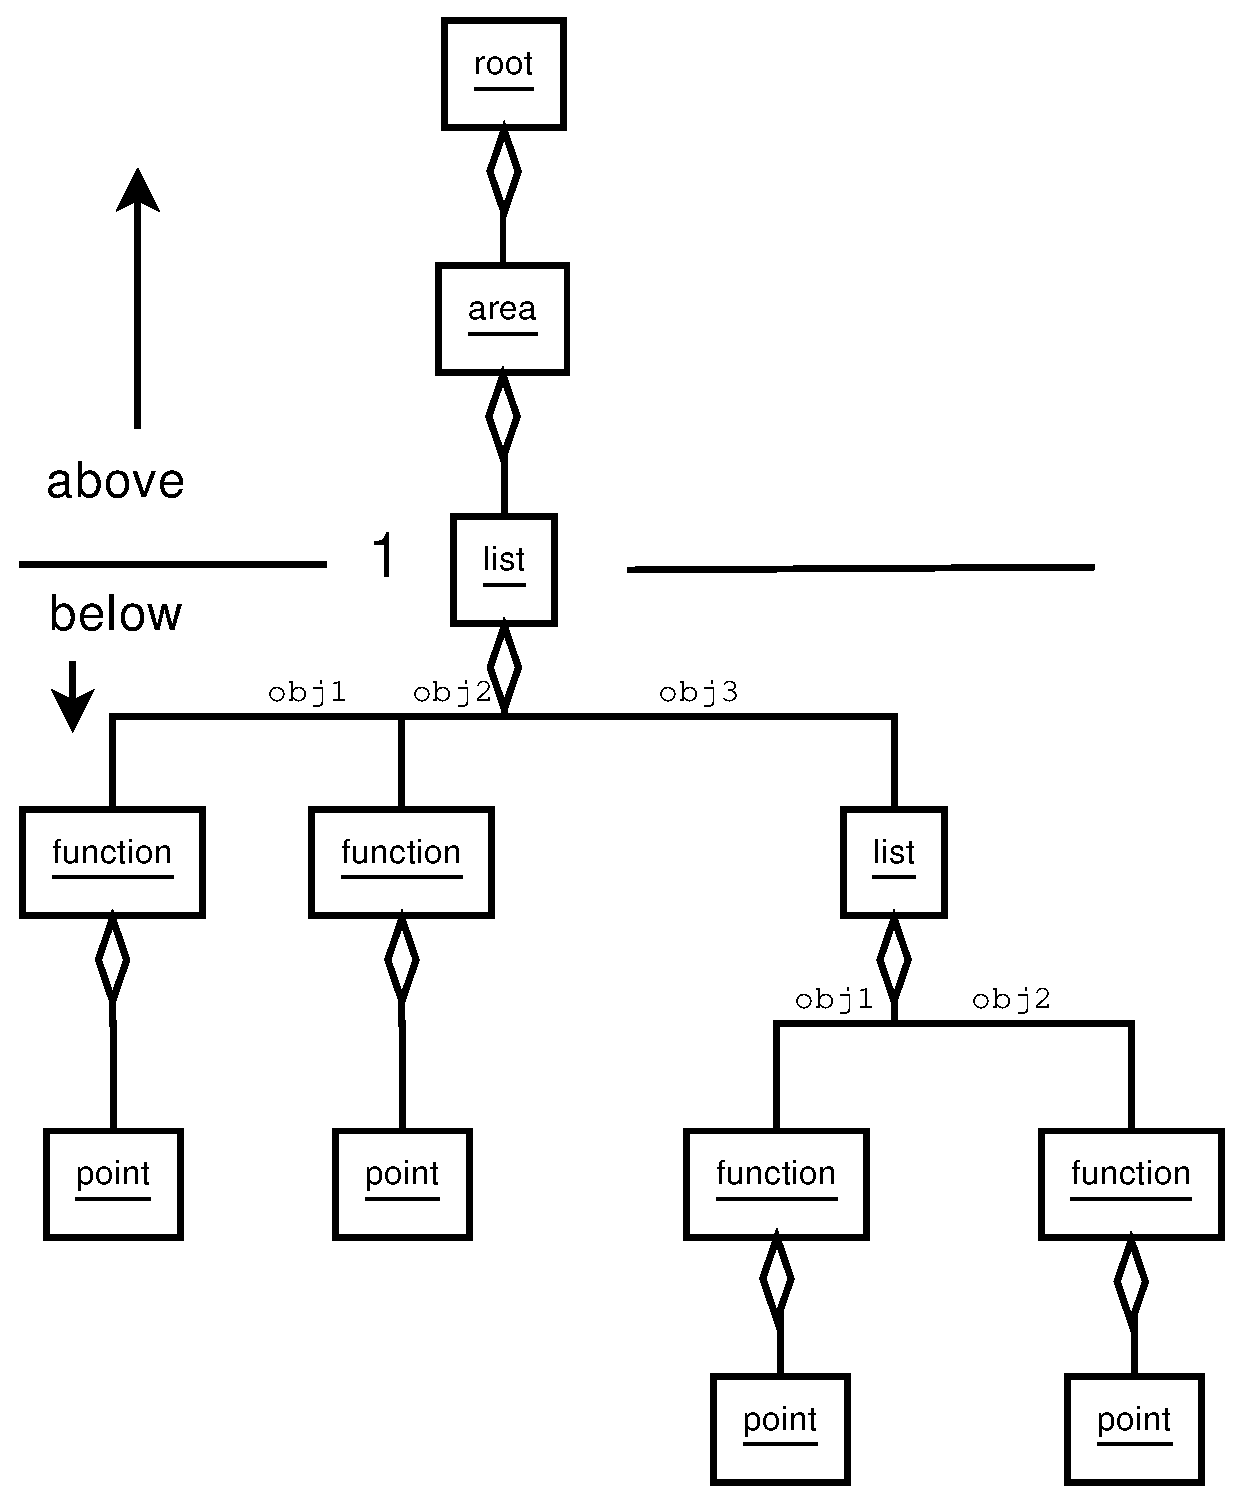
\includegraphics[scale=0.5]{above_below}
\end{center}
\caption{Example for ``below'' and ``above'' in a Fib object}
\label{figDirectionFibElements}
\end{figure}


\subsection{Order of the Fib elements}\index{order!Fib elements}
\label{secOrderFibElements}

On the definitions of ``below'' and ``above'' in a Fib object the order of Fib elements is established. To each Fib element in the complete Fib object an unique natural number is assigned. If in a Fib object $N$ elements exist, the numbers $1$ to $N$ will be assigned to the Fib elements in the Fib object. Fib elements below a Fib element are assigned to higher values.

If a list element subobject $Obj_U$ has a higher number $U$ as another subobject $Obj_K$ ($U>K$) of the list element, it also contains Fib elements with higher numbers as the Fib elements in $Obj_K$. The root-elements are treated the same way in the order as list elements, with the main-Fib-object as the first subobject after which the sub-root-objects follow in ther succession (in the root-element).

The same applies for any other branch element. The above defined syntax determines the order of the subobjects.

In figure \ref{figOrderFibElements} a sample object with the corresponding numbers (next to the elements) for the order of the Fib element is shown.

\begin{figure}[htbp]
\begin{center}
  \includegraphics[scale=0.5]{order_elements}
\end{center}
\caption{Example: Order of the Fib elements}
\label{figOrderFibElements}
\end{figure}


\subsection{Order of particular Fib elements}\index{Order!particular Fib elements}

Also Fib elements of a given typs are assigned to natural numbers of an order for there type. These orders are based on the order of the Fib elements. If in a correct Fib object $N$ Fib elements of a type exist, the numbers $1$ to $N$ are assigned to the Fib elements of this type. If to a Fib element $Elm_1$ in the order of the Fib elements a higher value is assigned (as to another Fib element $Elm_2$ of the same type), so it ($Elm_1$) is assigned to a higher value in the order of the Fib elements of the same type (than the other Fib element $Elm_2$).

In figure \ref{figOrderSpecialFibElements} an example object with the corresponding numbers (next to the elements) for the order of particular Fib element is shown.

\begin{figure}[htbp]
\begin{center}
  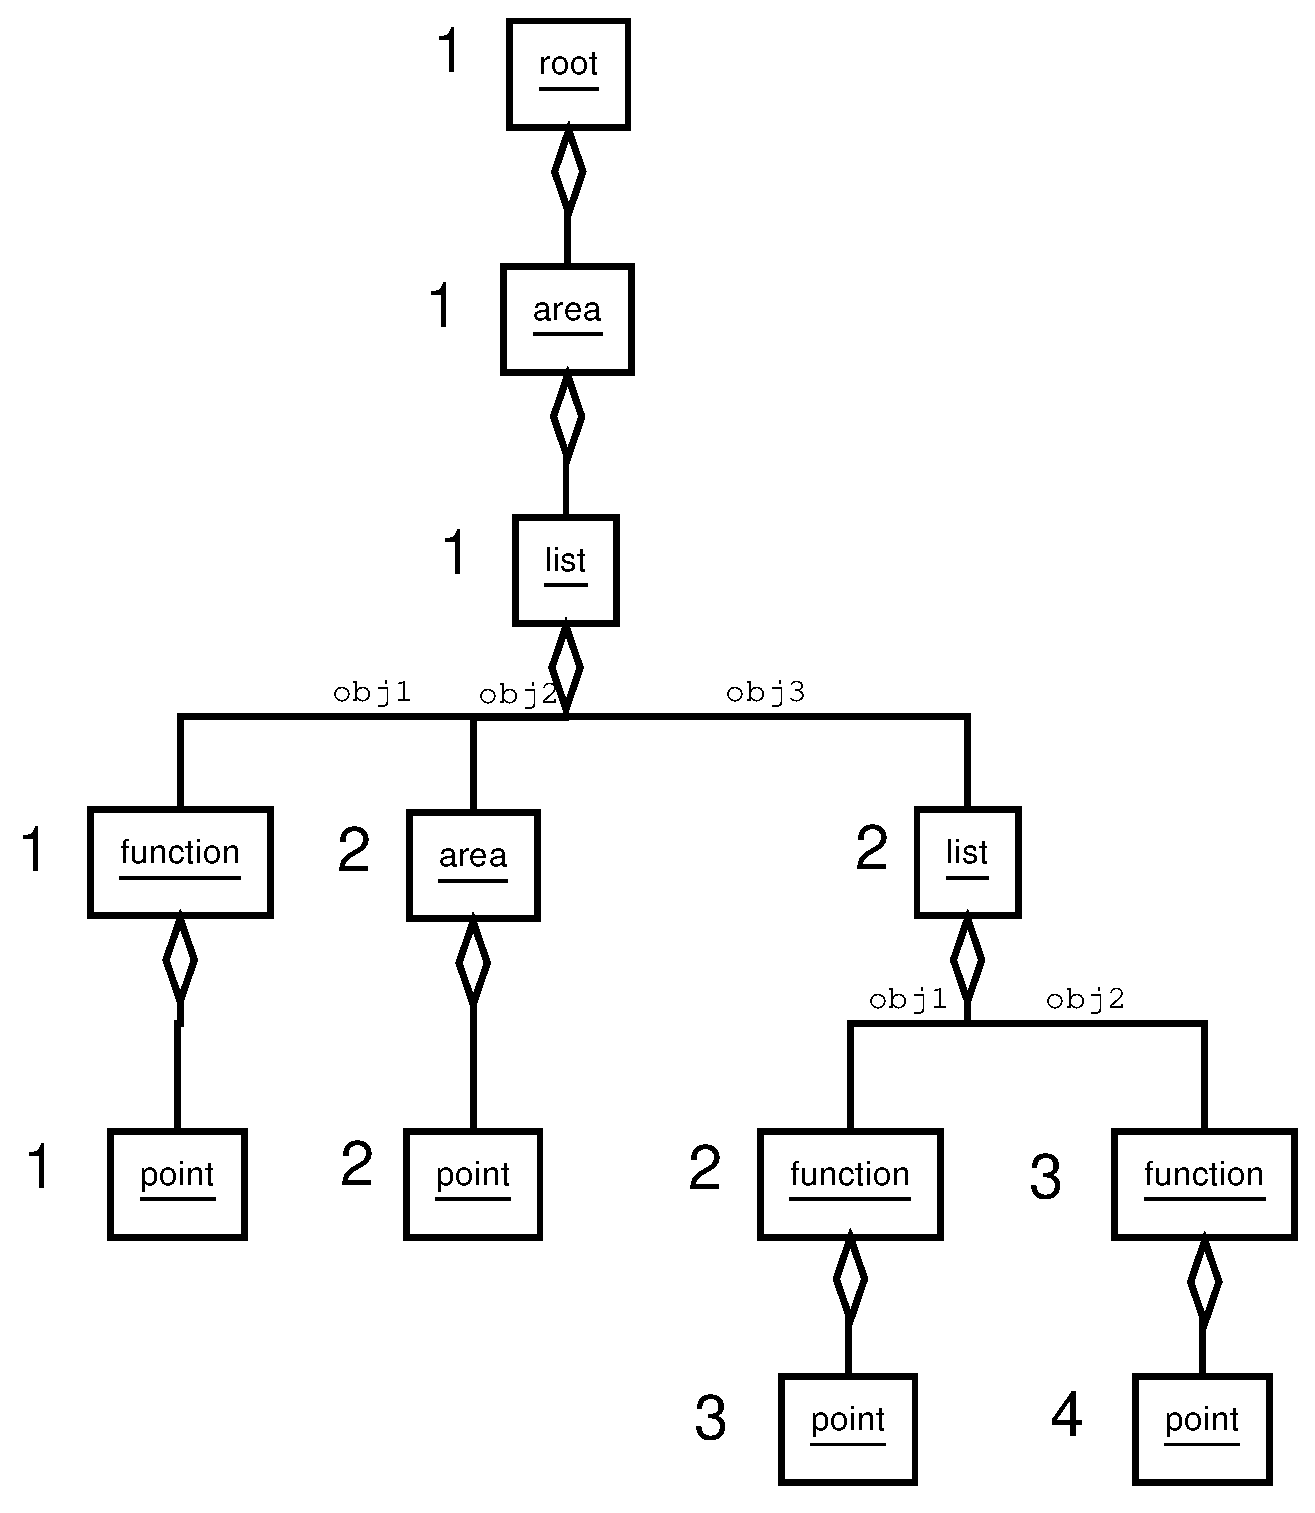
\includegraphics[scale=0.5]{order_special_elements}
\end{center}
\caption{Example: Order of particular Fib elements}
\label{figOrderSpecialFibElements}
\end{figure}


\subsection{Order of move points}\index{move points}\index{order!move points}

Another order applies to all Fib elements that can be moved. These are called move points.
The orders of the move points is based on the order of the Fib elements. If in a complete Fib object $N$ move points (movebel Fib elements) exist, the numbers $1$ to $N$ are assigned to these movebel Fib elements. If to a movebel Fib element $Elm_1$ in the order of the Fib elements a higher value is assigned (as to another movebel Fib element $Elm_2$), so it ($Elm_1$) is assigned to a higher value in the order of the movebel Fib elements (than the other Fib element $Elm_2$).

\bigskip\noindent
Fib elements, which can be moved and represent move points, are all limb elements (they are containing exactly one subobject):
\begin{itemize}
 \item property element (see section \ref{fibProperty} on page \pageref{fibProperty})
 \item comment element (see section \ref{fibComment} on page \pageref{fibComment})
 \item area element (see section \ref{fibArea} on page \pageref{fibArea})
 \item functions (see section \ref{fibFunction} on page \pageref{fibFunction})
 \item Fib elements, to retrive domain properties (see sectiont \ref{fibDomeinProperties} on page \pageref{fibDomeinProperties})
 \item set-element (see section \ref{secFibSetElement} on page \pageref{secFibSetElement})
 \item matrix element (see section \ref{secFibMatrixElement} on page \pageref{secFibMatrixElement})
\end{itemize}

\bigskip\noindent
Fib elements, which can't be moved and don't represent move points, are:
\begin{itemize}
 \item all leaf elements:
 \begin{itemize}
  \item points (see section \ref{fibPoint} on page \pageref{fibPoint})
  \item Fib elements to call external subobjects (see section \ref{fibSubobject} on page \pageref{fibSubobject})
 \end{itemize}
 \item all branch elements:
 \begin{itemize}
  \item root-element (see section \ref{fibRootElement} on page \pageref{fibRootElement})
  \item list element (see section \ref{fibList} on page \pageref{fibList})
  \item the Fib element, to call external objects (see section \ref{fibExtObject} on page \pageref{fibExtObject})
  \item conditions with the if-element (see section \ref{secFibIf} on page \pageref{secFibIf})
 \end{itemize}
\end{itemize}

In figure \ref{figOrderMovePoints} an example object with the corresponding numbers (next to the elements) for the order of move points is shown.

\begin{figure}[htbp]
\begin{center}
  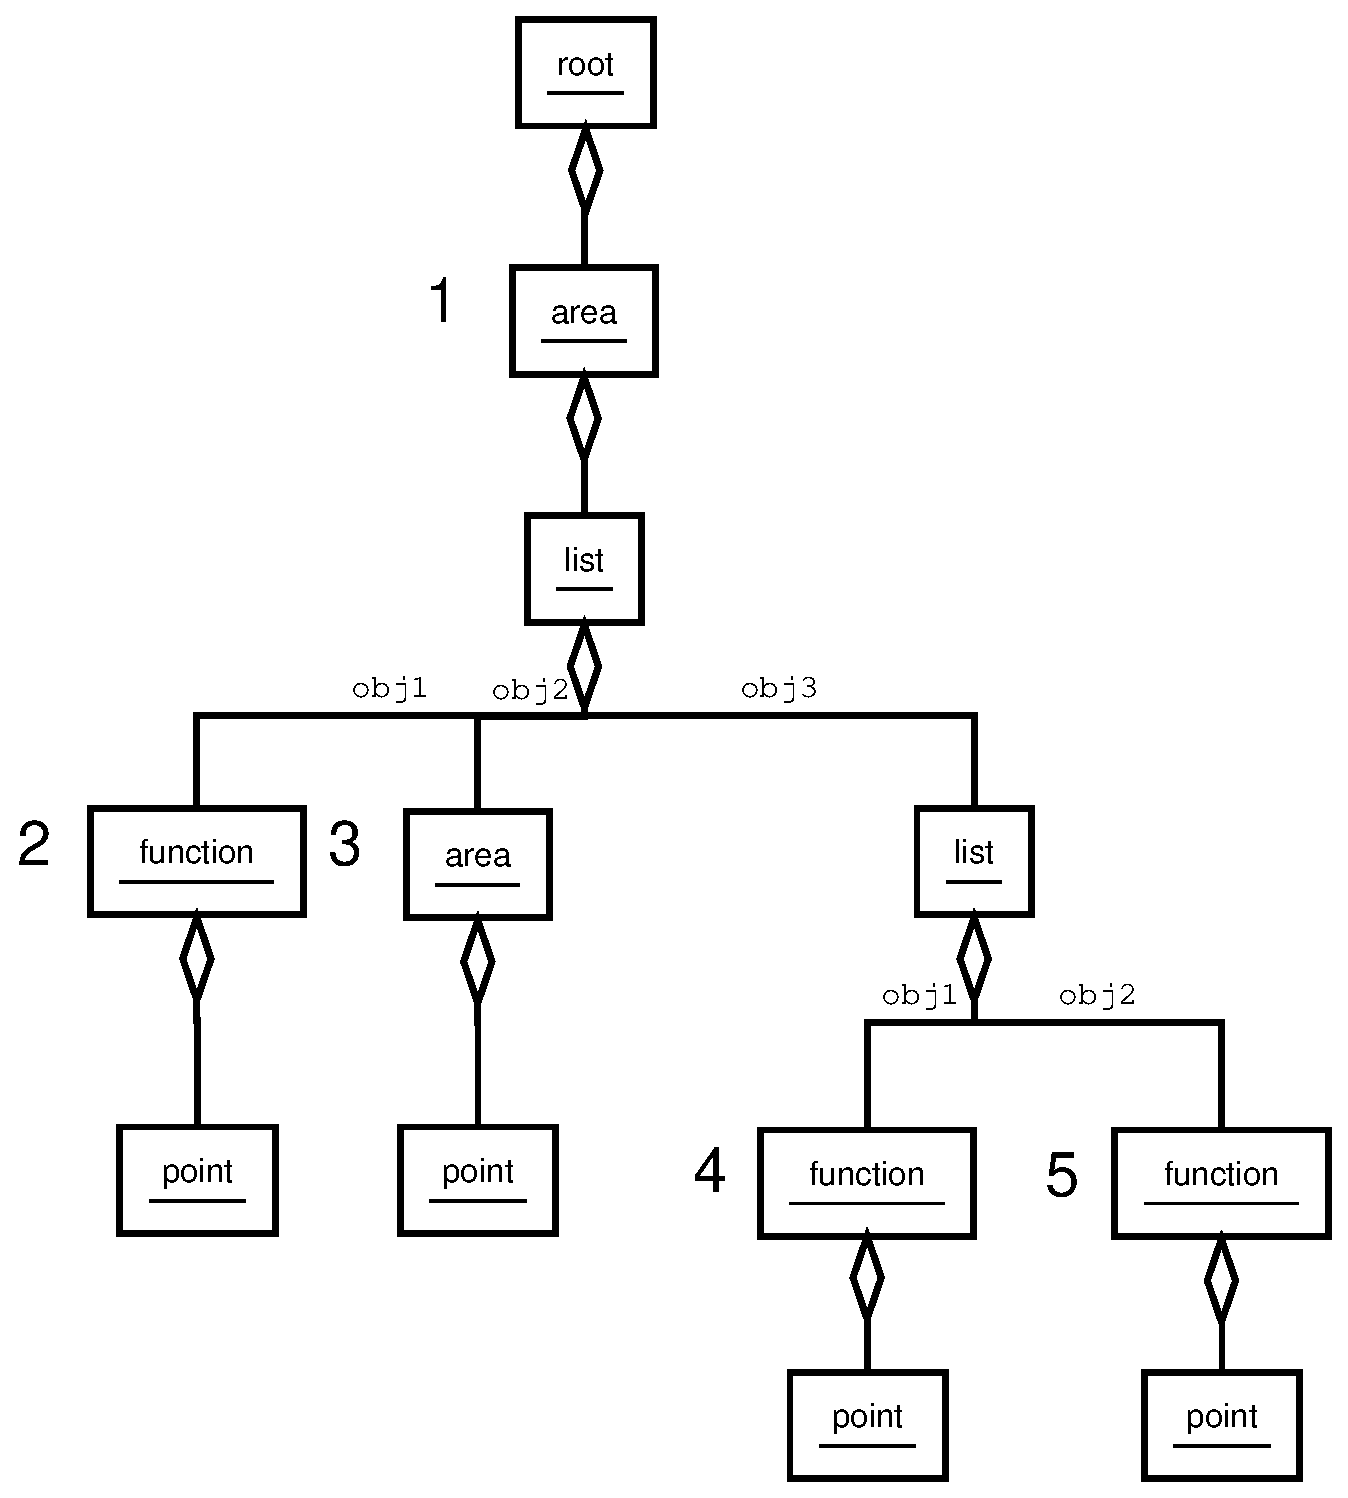
\includegraphics[scale=0.5]{order_move_points}
\end{center}
\caption{Example: Order of move points}
\label{figOrderMovePoints}
\end{figure}


\subsection{Definition: part object}\index{part object|(}

Any object that is a whole branch (e. g. a sub-list object, main-Fib-object or sub-root-object) of a branch element is part of a part object. Furthermore, to the part object belong all root-elements, in which it is contained or which it uses for external objects. Even Fib elements, which define variables that are used in the part object, belong to it.
The union of two part objects is again a part object.
The complete Fib object itself is also a part object.
A part object can always be evaluated to a multimedia object.

A \textbf{genuine part object}\index{part object!genuine} is a part object, that is not the (complete) Fib object itself.

A \textbf{simple part object}\index{part object!simple} is a genuine part object, that contains only one leaf with one point object.

A \textbf{coherent part object}\index{part object!coherent} is a genuine part object that contains the whole object of one branch (subobject), of just one branch element (e. g. list element or root-element) and the required elements above it. In particular, every simple object is a coherent subobject.

To create a coherent part object, one branch element (for example list element or root-element) from the complete Fib object can be deleted and replaced by one of the subobjects contained in it. The resulting subobject must of course be correct, to be a coherent part object. (For example, if the main-Fib-object of a root-element is deleted, the result isn't a coherent part object. Also if a sub-root-element is deleted, and the next above main-Fib-object is replaced by its main-Fib-object, the domains of the replace root-element should be adapted by the next root-element.)

With figure \ref{figOrderFibElementsPartobjects} this definition is illustrated with an example of a Fib object. In the following, some examples of different types of part objects in Figure \ref{figOrderFibElementsPartobjects} are being given, for the Fib elements their numbers (from the Fib element order respectively figure \ref{figOrderFibElementsPartobjects}) are given. Furthermore, it is establish that the point element with the number $10$ does not use the variable that is defined by the area element with the number $2$. All other variables are needed in the points, which are below the respective variable definitions.


\begin{figure}[htbp]
\begin{center}
  \includegraphics[scale=0.5]{order_elements}
\end{center}
\caption{Example object for part objects}
\label{figOrderFibElementsPartobjects}
\end{figure}


\bigskip\noindent
Part objects:
\begin{itemize}
 \item 1; 2; 4; 5
 \item 1; 2; 6; 7
 \item 1; 2; 3 (just subobjects $1$ and $2$); 4; 5; 6; 7
 \item 1; 9; 10
 \item 1; 2; 8; 9; 10; 11; 12
 \item 1; 2; 3 (just subobjects $1$ and $3$); 4; 5; 8; 9; 10; 11; 12
 \item 1; 2; 3 (just subobjects $1$ and $3$); 4; 5; 11; 12
 \item (all Fib elements) 1; 2; 3; 4; 5; 6; 7; 8; 9; 10; 11; 12
\end{itemize}

Genuine part objects:
\begin{itemize}
 \item 1; 2; 4; 5
 \item 1; 2; 6; 7
 \item 1; 2; 3 (just subobjects $1$ and $2$); 4; 5; 6; 7
 \item 1; 9; 10
 \item 1; 2; 8; 9; 10; 11; 12
 \item 1; 2; 3 (just subobjects $1$ and $3$); 4; 5; 8; 9; 10; 11; 12
 \item 1; 2; 3 (just subobjects $1$ and $3$); 4; 5; 11; 12
\end{itemize}

Simple part objects:
\begin{itemize}
 \item 1; 2; 4; 5
 \item 1; 2; 6; 7
 \item 1; 9; 10
 \item 1; 2; 11; 12
\end{itemize}

Coherent part objects:
\begin{itemize}
 \item 1; 2; 4; 5
 \item 1; 2; 6; 7
 \item 1; 9; 10
 \item 1; 2; 11; 12
 \item 1; 2; 8; 9; 10; 11; 12
\end{itemize}


\subsection{Order of the coherent part objects}
\label{secOrderPartobjects}

There is an order on the coherent part objects as well. This will hereinafter also called order of part objects, as there are no own orders for the other types of part objects.

The orders of the (coherent) part objects is based on the order of the Fib elements. If in a complete Fib object $N$ (coherent) part objects exist, the numbers $1$ to $N$ are assigned to these part objects.
The greater the number of a coherent part object, the greater is the smallest number in order of the Fib elements, of the Fib elements in it.
Or: If to the top most Fib element of the subobject, which defines the coherent part object, a higher value assigned, than the defined part object is also associated with a higher value.

In figure \ref{figOrderPartobjekts} an example object with the corresponding numbers (next to the defining subobjects of the part objects) for the order of (coherent) part objects is shown.

\begin{figure}[htbp]
\begin{center}
  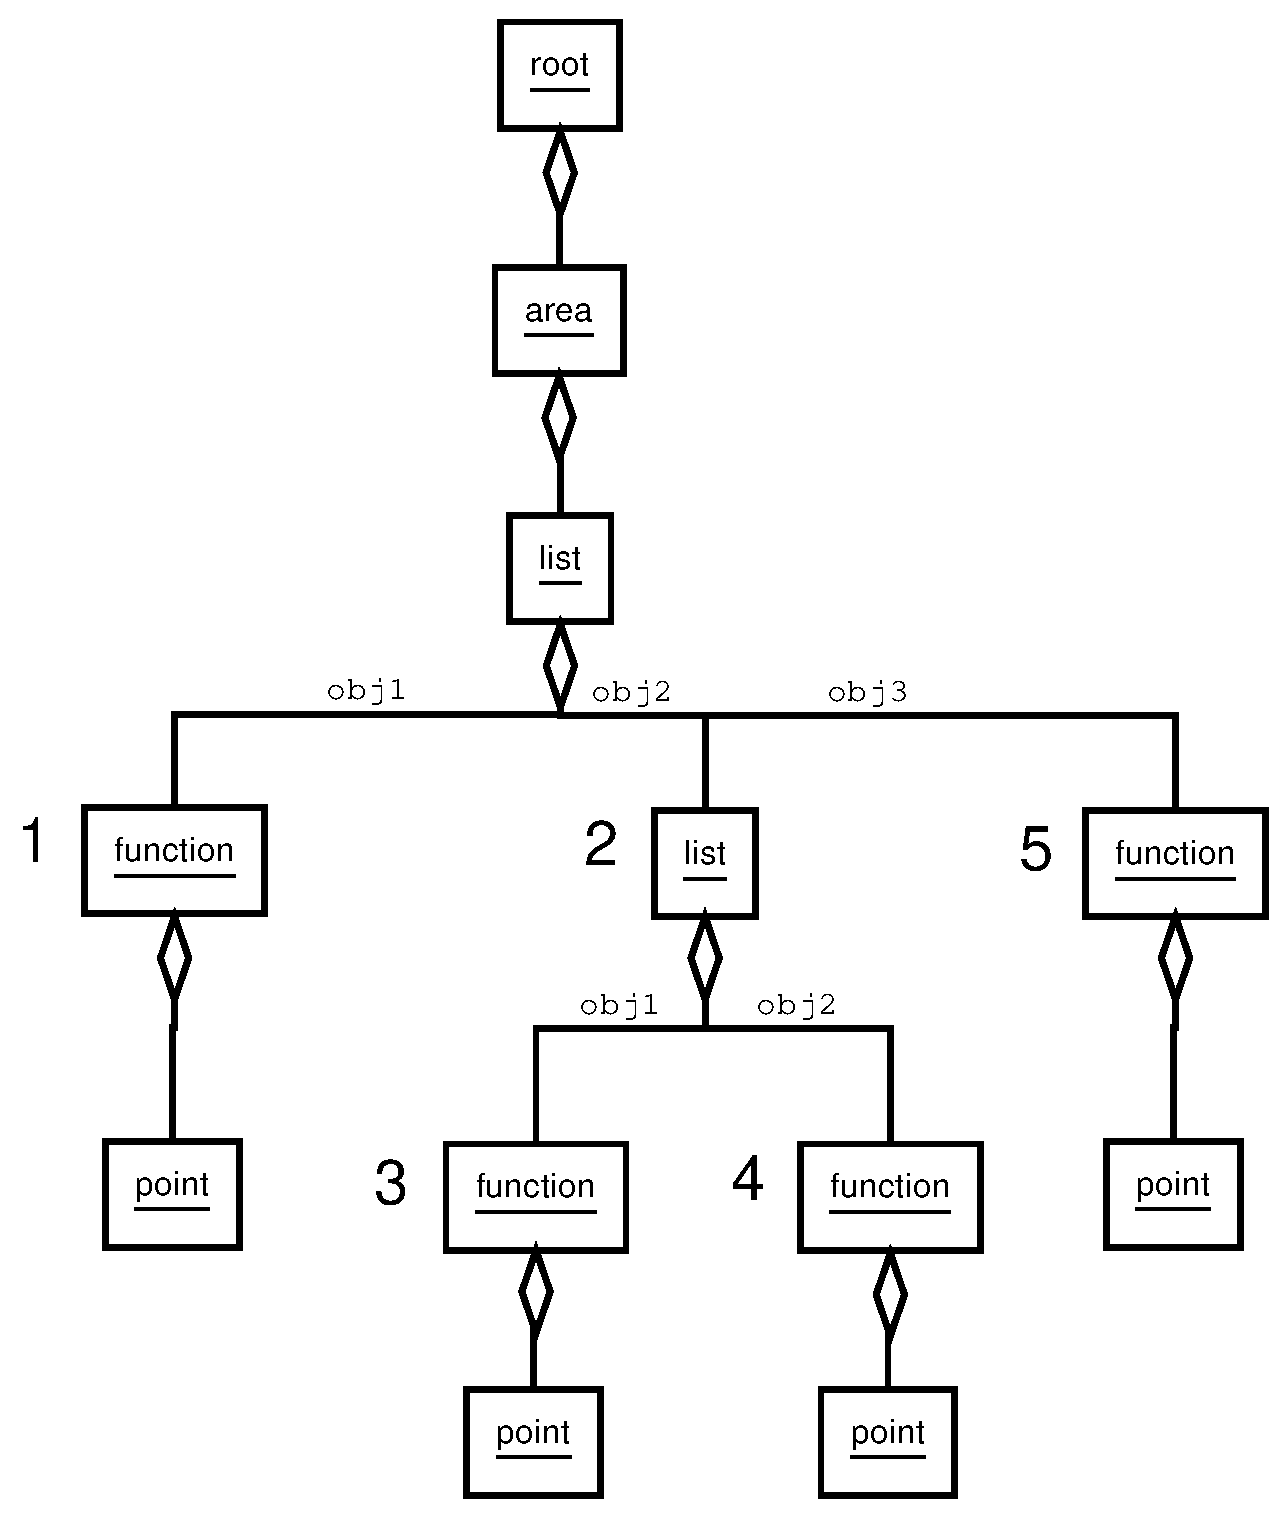
\includegraphics[scale=0.5]{order_partobjects}
\end{center}
\caption{Example: Order of (coherent) part objects}
\label{figOrderPartobjekts}
\end{figure}


\index{part object|)}


\subsection{Definition of Fib multimedia object}\index{Fib multimedia object}

If the expression Fib multimedia object is used, the Fib object with focus on the multimedia object it represents is meant.


\subsection{Definition of correct Fib multimedia object}\index{Fib multimedia object!correct}

A correct Fib multimedia object is a Fib object, that fully reflects the original multimedia object, which it should represent. So, if the multimedia object that the Fib object represents, and the original multimedia object are compared, no difference between them can be found.



%TODO: in welche Sprache kontextfrei oder regulär?





%
% Copyright (c) 2008 Betti "Osterholz
%
% Permission is granted to copy, distribute and/or modify this document
% under the terms of the GNU Free Documentation License, Version 1.2 or
% any later version published by the Free Software Foundation;
% with no Invariant Sections, no Front-Cover Texts, and no Back-Cover Texts.
%
% A copy of the license is included in the file ``fdl.tex'' .
%


\section{Theoretical statements for the Fib multimedia description language}
\label{secTheoreticFib}

Some theoretical statements for the Fib multimedia description language will follow, for wich, because of lack of time, usually not a complete proof is given. With these statements a better understanding of the Fib multimedia language should be provided.


\subsection{Power of the Fib multimedia language on images}
\label{secPowerOfFibOnPictures}

With the Fib multimedia language all as raster graphics displayable images can be represented. Images, that are displayed as raster graphics, are the most commonly used images in the digital data processing. These include Windows bitmap (BMP; file extension: .bmp), JPEG File Interchange Format (JFIF, file extension: .jpg) and Portable Network Graphics (PNG, File Extension: .png).

With using only the point element and the list element alone all possible raster graphics can (already) be represented.

\bigskip\noindent
\textbf{Proof:}
A raster graphic (euclidean, two dimensional, discrete) can be represented as a matrix, the column indicats the x coordinate, the lines the y coordinate of the point and the values specify the colors of the points. The number of dots in the raster image is finite. To represent these points in the Fib multimedia language, a root-element have to be created that contains the properties of the raster graphic (size and dimension domain etc.). In this root-element a main Fib object, wich is a list element, is inserted, which contains for each point of the image a subobject. This subobject consists only of a property element, which encodes the color of the point, and one contained point element, which encodes the position of the point. So there is for every point in the raster graphic a corresponding point in the generated Fib object, so that the Fib object represents the raster image.

A mapping into the Fib multimedia language can for example be implemented by the algorithm shown in listing \ref{alleBild} (pseudo-C).

\begin{flushleft}
The indexing of the matrix begins with (0.0).

The color value of coordinates (x, y) can be determined with \verb|matrix[ x, y ]|. With the function \verb|getColorVector()| a Fib color vector is generated from the matrix color value.

The syntax of the Fib objects corresponds to the in section \ref{partFibLanguage} on page \pageref{partFibLanguage} discussed possible syntax.

\end{flushleft}

\begin{lstlisting}[language=C, numbers=left, frame=single, caption={Algorithm to generate a correct Fib object from an image matrix}, label={alleBild}, breaklines, basicstyle=\footnotesize\ttfamily, numberstyle=\tiny]
void translate( matrix ){

   int xmax = number of columns of the matrix;
   int ymax = number of lines of the matrix;
   Fib_Object_Pointer obj = new root();

   //set the properties of the raster graphic
   obj->setPicture( xmax, ymax, colorScheme );

   list mainList = new list()

   obj->insertMainObject( mainList )

   for( int x = 0; x == xmax; x = x + 1 ){

      for( int y = 0; y == xmax; y = y + 1 ){
         mainList->insertObject( property( getColorVector( matrix[x,y] ) , p( (x,y) ) ) );
      };
   };
};
\end{lstlisting}
\bigskip\noindent
Since the expansion with functions and other elements is optional, a correct Fib object is generated with the specified algorithm.

\bigskip\noindent
For each point in the matrix there is a same-colored point in the Fib object with the corresponding coordinate, but there are no points in Fib object that are not present in the matrix, because each coordinate of the matrix is traverse with the two ``for'' loops. Thereby a point in the Fib object is added for each coordinate and thus for every point in the raster graphic. Thus for every point in the raster graphic a corresponding point in the Fib object exists.
Since only coordinates of the matrix are traverse in the ``for'' loops and only for them corresponding points are included in the Fib object, there are only points that appear in the matrix and hence only points in the Fib object, which also occur in the raster graphic.
So there are only the points from the original raster graphic in the Fib object and no more.
Thus the Fib object and the original the raster graphic represent (/shows) the same raster graphic. Therefore, all raster graphics are representable with the Fib multimedia language.

A Fib object generated by the algorithm, that represents an original raster graphic, is an upper limit to the minimum size of possible corresponding Fib objects. This means, each raster graphic can be represented by a Fib object, that is as big as the Fib object for the raster graphics that was generated with the above algorithm, that is the Fib object generated. But there are likely even shorter Fib objects for raster graphics.

\begin{flushleft}
With that the minimum size of a Fib object for a raster graphic is maximal:

$Fib\_max_{min}$ = (number of pixels in the image) $* [$(size of a point element) + (size of a property element for the appropriate color scheme)$]$ + (size of a list element)+ (size of a root-element with values set)

\bigskip\noindent
Example: You want to shown an image of 8 x 8 = 256 pixels with 3 bytes for the color (RGB), 1 byte for the position (for each direction x and y 4 bits = 8 possible values) and 1 byte for the object name (for example ``l'' for the list elements and ``p'' for the point elements). Parentheses are not needed, because all parts have a fixed length. (The assumptions about the sizes of the Fib object elements are estimated here. In a implementation, better (/smaller) values are more likely.)

\begin{itemize}
 \item A point element requires 2 bytes (1 byte position + 1 byte element name).
 \item For a property element 4 bytes are needed (3 bytes color + 1 byte element name).
 \item For a list element 9 bytes are needed (8 bytes for specifying the number of subobjects + 1 byte element name).
 \item The root-element requires 256 bytes. (Since many parts of the root-element are empty and only the domain for two dimensions and the RGB color domain must be specified, 256 bytes should be enough.)
\end{itemize}

\bigskip\noindent
Calculation:
$256 (pixel) * (2 bytes + 4 bytes) + 9 bytes + 256 bytes = 1801 bytes$

\bigskip\noindent
So the image can definitely be displayed with a 1801 byte long Fib object. But there are other shorter Fib object representations possible. The 1801 bytes are thus the upper limit for the minimum size with which the image can be represented by a Fib object.

\bigskip\noindent
For comparison: The memory requirements of a raster image as a bitmap (only point information) is at least
(Number of pixels in the image) * (size of a color value)

\bigskip\noindent
For the above example it results in: $256 (pixel) * 3 bytes = 768 bytes$

\bigskip\noindent
That's about half of the 1801 byte limit on the minimum Fib object representation.

\bigskip\noindent
In that the matrix is extended to three dimensions, the statement about the representability of all raster images can be easily extended to sequences of raster images (such as the images of movies).

\end{flushleft}


\subsection{Cardinality of Fib}

\textbf{Theorem: The set of possible Fib objects is countable infinite.}

\bigskip\noindent
Sketch of proof for ``countable'':

\noindent
Every Fib object can be represented with a finite number of letters, and thus bits or numbers, and the amount of these is countable.
This follows from the fact, that the number of Fib elements in a Fib object is always countable and every Fib element consists of countably many parts, which are themselves countable, there are for example only integer or rational numbers, and also the number of variables is countable.

\bigskip\noindent
Sketch of proof for ``infinite'':

\noindent
All natural numbers can be represented by Fib objects. In the following a possible representation of any natural number with a Fib object is described.

A point object itself is the natural number 0 .
If a Fib object is inserted in a new function element the resulting Fib object is the successor of the original Fib object.
In this manner the 0 and the successor function can be reproduced in the Fib multimedia language, and all natural numbers can be represented. Since the set of natural numbers is infinite, the amount of Fib objects is also infinite.

\bigskip\noindent
Even every multimedia object can be represented by a countable infinite set of Fib objects, because to a Fib object, that represents a multimedia object, any Fib object can be attached with the help of a list element, as long as the multimedia object representation is not changed. For example, to a Fib object a copy of itself using a list element can be as often attached as needed, without changing the multimedia object.


\subsection{Any complete Fib object can be represented as a multimedia object}
\label{alleBilder}

It is shown in this section, that it is always possible to interpret (to translate into a multimedia object) any complete Fib object (see section \ref{secFullFibObject} on page \pageref{secFullFibObject}) in a way, that only valid multimedia objects of a certain type (e. g. RGB images with 100 x 100 pixels) can result. In which the limitations with regard to the multimedia data, as already mentioned, are assumed, that the multimedia data can be represented as properties of points of a finite, euclidean and discrete (there are smallest units) space. This restriction is not very large, because they (almost) excludes non of the presently common multimedia data. The multimedia data may therefore represent images, sound or movies.

With the restriction that the distance / difference between two properties of the same type can always be determined as a numerical value, two multimedia objects with the same dimensions can be always compared. Two multimedia objects have the same dimensions, if for each point in the first multimedia object exactly one corresponding point in the other multimedia object exists.

The requirement of the complete Fib object is necessary to ensure that the Fib object can be always evaluated. Since the completeness of an Fib object can be check with the syntax shown in part \ref{partFibLanguage}, if a Fib object is complete can always be determined. Incomplete Fib objects should not be generated by the algorithms or the genetic operators.

If the dimensions of a Fib object are adapted to that of a multimedia object (this should be always possible), the Fib object is always comparable with the multimedia object, because it can itself be always presented as a multimedia object, and two multimedia objects with the same dimensions can always be compared to each other and the similarity to each other can be evaluated.

Note: This is advantageous for genetic algorithms. In some other forms of representation that are generated by genetic algorithms, invalid objects (e. g. programs) arise, where a more accurate evaluation / comparison is not possible. A population in this format can contain, for example, a large class of objects that are invalid, which are all equally bad and are therefore considered same in the selection process. If the population consists only of invalid individuals, the selection of a better individual is impossible. The genetic algorithm is then on a (fitness) plane, from which it can only find away with great difficulty.

\bigskip\noindent
Proof that every correct Fib object can be represented as a multimedia object (of a specific type, such as a picture):
The starting point is that a multimedia object (euclidean, two-dimensional, discrete) can be represented as a finite set of points with their (finitely many) properties. Since there are only finitely many points with only finitely many properties, such a finite set is always constructible.

Such a finite set of points with their (finitely many) properties is also generated by a correct Fib object. Points of the set that are too much to represent a multimedia object, will be deleted from the set. Points that are missing in the set to represent a multimedia object are inserted into the set. Properties of the points that are too much to represent a multimedia object will be deleted. Properties, which are missing at points to represent a multimedia object, are added and set with their default values (e. g. the zero values of their domains). In this way a finite set of points is created with their (finite many) properties that can be represented as a multimedia object.

\bigskip\noindent
Example: The Fib object should represent an RGB image with 100 x 100 pixels. For this the dimensions of the Fib object are adjusted to cover these 100 x 100 pixels in horizontal and vertical direction. That is, if the dimension (horizontal or vertical) already exists, the domain of each direction is adjusted, so that it covers at least 100 values at regular intervals. So that to each pixel a value is assigned. If a dimension (/ direction) is missing, it will be created with the appropriate domain and in all points for the dimension the standard value of 0 will be set. In this case there is no point with other values than the default value for this dimension. Dimensions that are too much, are deleted from the root elements and the points. The evaluation of the resulting Fib object produces a set of points with their properties. During evaluation, the smallest value of $W_{min}$ of each dimension in the Fib object is assigned to the value 0 as the coordinate in the set, the second smallest one to 1 as the coordinate, etc.

From this set now all points are deleted that are not within the 100 x 100 pixels boundary (points for which a coordinate respectively value is less than 0 or greater than 99). For all coordinates, which are still missing (missing points, where the values respectively the coordinates is between [including] 0 and 99), points are inserted. All properties that are not RGB colors will be deleted. To all points that have no property for RGB colors, the default color $(0, 0, 0)_{colorRGB}$ is assigned. The resulting set contains for each point in the RGB image with 100 x 100 pixels a point with RGB color, but no other points or properties, and thus represents an RGB image with 100 x 100 pixels.

This can then be compared with other RGB images with 100 x 100 pixels and rated in relation to them.












%TODO prio 2 (secPowerOfFibOnPictures): \input{fib_aussagen_theoretische_en}
%%\input{fib_annahmen_en}%TODO
%
% Copyright (c) 2011 Betti Österholz
%
% Permission is granted to copy, distribute and/or modify this document
% under the terms of the GNU Free Documentation License, Version 1.2 or
% any later version published by the Free Software Foundation;
% with no Invariant Sections, no Front-Cover Texts, and no Back-Cover Texts.
%
% A copy of the license is included in the file ``fdl.tex'' .
%

%path for pictures
\graphicspath{{./stock_environment/}}
\graphicspath{{./stock_environment/}{../stock_environment}}


\newpage
\part{The genetic algorithm}\index{genetic algorithm}\index{algorithm}
\label{secGeneticAlgorithmDesign}

In this section, general design decisions and initial analysis for the genetic algorithm are established.
The realized genetic algorithm is flexible and expandable designed.

The genetic algorithm is also an evolutionary algorithm. The term ``genetic'' refers to the ability of the algorithm to encode information of two or more individuals in a new individual and that it is working on information that code the (multimedia) object and do not represent those objects directly.

The algorithm is used to generate Fib objects, which represent a multimedia object as well as possible. The algorithm is given a particular multimedia object, for that it generates Fib objects /individuals, of which good will be selected. The creation of new individuals may also include analysis of the multimedia object and the use or analysis of information from other individuals. Which individuals are good, can be decided by the given parameters (by the evaluator for individuals).

\bigskip\noindent
The algorithm consists of five separate parts:
\begin{itemize}
 \item the core algorithm
 \item the evaluator for individuals
 \item the mortality rating algorithm
 \item the evaluator for operators
 \item the set of operators
\end{itemize}

In Figure \ref{figGeneticAlgorithmus} a sketch for the flow diagram for the genetic algorithm is shown.

\begin{figure}[htbp]
\begin{center}
  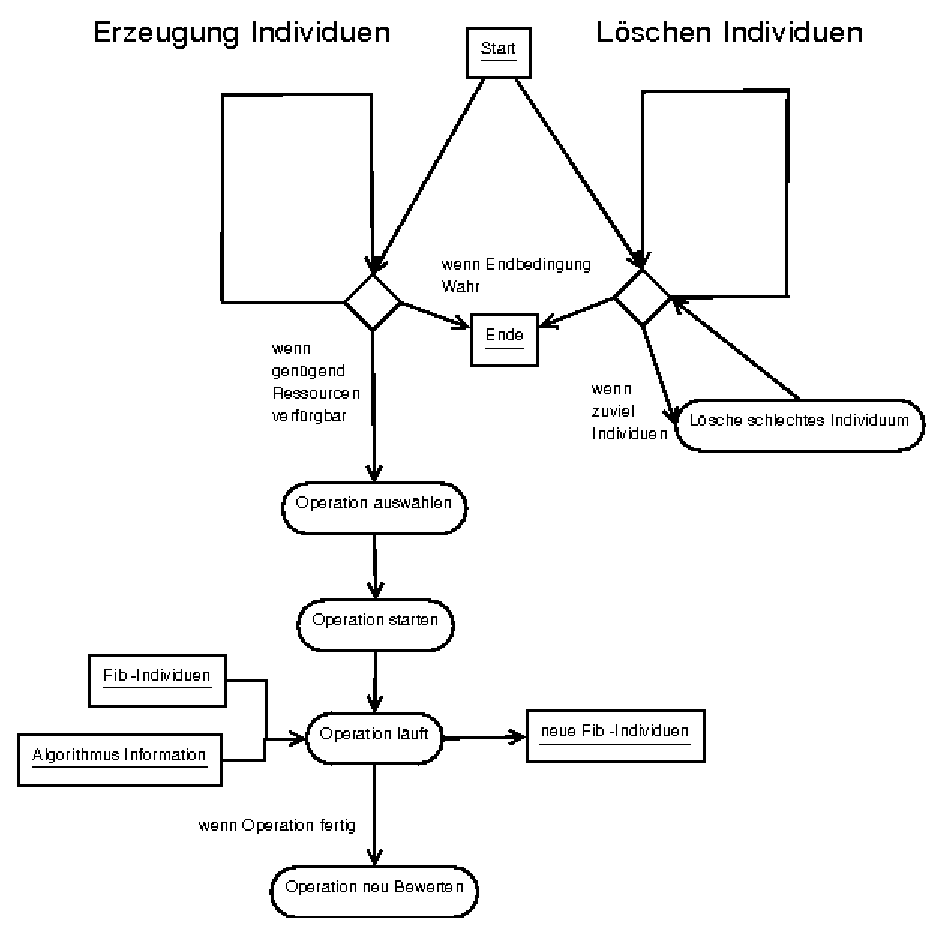
\includegraphics[scale=0.4]{algorithmus}
\end{center}
\caption{Flow diagram of the genetic algorithm}
\label{figGeneticAlgorithmus}
\end{figure}

In the following the single Fib objects are called individuals. The set of all individuals, who are existing at a time in the algorithm, is calle population.


\section{Core algorithm}\index{core algorithm}

The core algorithm uses the evaluator and the operators to realize the genetic algorithm. It is simple and flexible.

The evaluators for individuals or operators are (with the help of parameters) interchangeably.

\bigskip
The core algorithm includes the main loop of the genetic algorithm, which calls the operators and generates the individuals.

The second loop in the algorithm is the selection loop. It will delete individuals.

\bigskip
In addition, the core algorithm provides functions for the operators. The operators are called by the core algorithm through a method, that is the same for all operators. After that, the operators can get, with the help of the functions of the core algorithm, the algorithm specific values, e. g. such as individuals, which the operations will use. In this way, the operators will always look the same in each case for the core algorithm, and the core algorithm does not need any logic specific to a particular operator. Thereby future adjustments to the operators are simplified, because not the interface of all operators have to be be adjusted, but only the functions, which are provided by the core algorithm.

The calling method for the operators should be flexible, so that operators can be started concurrently and the algorithm don't have to wait for the completion of each operation. The operators should be run separately from the core algorithm and affect it only by the specified interface. A faulty operator should not lead to errors in or termination of the entire system.


\section{Evaluator for individuals}\index{evaluator!individuals}

The concrete evaluator algorithm should be simple to replace, so it can be adapted to various problems. The respective evaluation algorithm is needed to calculate the fitness of an individual.

With the help of parameters for special evaluators, they can be further adjusted (for example it can be adjusted, how important a small size compared to a fast evaluation of individuals is).


\subsection{The fitness of individuals}\index{fitness!individuals}

The fitness of an individuals is determined by different fitness factors.

One of the most important is, to what extent the individual is similar to the desired original multimedia data (such as the original image). The more the individual (or the phenotype of it) is similar to the original multimedia data, the higher the fitness should be and the lower is the error, which the individual has for the display of the original multimedia data.

This error (and thus the fitness of the individual) can be determine for example, with the sum of (the squared) differences (not defined points give the maximum error) of the colors of the points between the original image and the image produced by the individual, or through another self-determined distance.

If the fitness of separate part objects of the individual should be determined, this can be achieved, for example, by including in the evaluation only the area that is covered by the part object, the covered area and a border around this area or only the smallest square, which encompass this part object.

Another useful fitness factor is the size (increases with the number of elements) of the separate individuals, to give bigger individuals a lower fitness than smaller individuals, with the same error on the original multimedia data, and to prefer the smaller individuals.

A further fitness factor, which can be included, is the estimate of the time it takes to evaluate the individual for displaying the multimedia object (phenotype). In this way maybe even the execution speed of the algorithm can be increased.


\subsection{Selection by deletion of individuals}\index{Selection}

In order to spare the resources (memory, CPU time), it is necessary to limit the number of individuals (Fib objects) in the working process (individuals wich participate in the genetic algorithm). Therefore (if required) individuals have to be removed from it. In this process individuals with lower fitness are preferred.

There is therefore a \textbf{mortality rating algorithm}\index{mortality} for the algorithm. It determines the probability, with which a individual is deleted. To delete individuals, there is a separate loop in the algorithm, in which is tested, whether the maximum number of individuals is exceeded. If this is the case, individuals will be deleted, until the number of individuals is back on track (lower the maximum number of individuals). In this case individuals with a high mortality assessment by the mortality rating algorithm have a high probability of being deleted.

The mortality assessment is based on the assessment of the fitness of individuals. However, the mortality rating algorithm can be exchanged for other mortality algorithm or be controlled by parameters. For example, it is possible to declare some individuals to be immortal, so they can not be deleted. By declaring, for example, the $n$ ($n>0$) best individuals to be immortal, it can be avoided, that they will be deleted and thus that one of the best individuals will be lost.

The mortality algorithm can furthermore access via the operator interface the status information of the genetic algorithm, to determine, for example, the number of previously generated individuals.


\section{Evaluator for operators}\index{evaluator!operators}

To determine which operator to selected next, they are evaluated. Operators, which are rated better in a situation, have a higher probability of being selected respectively run in a similar situation.

\bigskip\noindent
The situation may include:
\begin{itemize}
 \item how many operations wher executed.
 \item of which nature the original multimedia object is (with the help of the domains for the environment in the root-elements of it):
 \begin{itemize}
  \item it contains colors
  \item it is monochrome
  \item it contains sound
  \item it is a film
  \item ...
 \end{itemize}
 \item the average (relative) fitness of individuals.
 \item the fitness of the best/worst individual.
 \item the standard deviation of fitness values in the population.
 \item the number of individuals.
 \item the operations that have been executed.
 \item ...
\end{itemize}

The different evaluation algorithms can be selected. Thus, different evaluation algorithms can be easily interchanged and compared.

To evaluate the operators, data of their previous execution may be kept permanently (by the seperate evaluators). In this way, the algorithm can learn from previous operator calls.

The evaluation of the operators should be system independent, ie. independent of the computer, on which the algorithm is running.

\bigskip\noindent
The evaluation criteria can be:
\begin{itemize}
 \item execution time of the operation
 \item reached deterioration or improvement
 \item reliability of the operator (Is always a result returned? Did it crashes sometimes?)
 \item ...
\end{itemize}


\section{The genetic operators for Fib}

The operators are to be seen separately from the genetic algorithm. It should be possible to add any number of operators for the use in the genetic algorithm, without having to adjust it.

Each operator has a unique identifier or ID, through which related values (such as its performance to date) can be associated to it.

An running operator is called operation.

The operations are intended to implement coding algorithms. Operators should therefore not be as simple as possible, but may as well involve complex algorithms.

The operators should also be numerous, and the algorithm is responsible for the selection of good operators. Therefore, it is also desirable to create own operators with good parts of other operators. In this case, both the original operators and the new operator, which contains the extracted parts, should be in the genetic algorithm.

For special applications, a genetic algorithm may be used, which set of operators was restricted to the most useful operators for this application.
Also, for a application useful operators can be combined to a (not genetic) algorithm, that uses them in determinated way.


\subsection{Reproduction}

In the general ``reproduction'', a individual is choosen from the population, preferably a individual with an high fitness, than it is copied and modified by one operation. At the end it is added to the population. It can also be checked, if it is a ``new'' object (if there is no equal object in the population) and just added in this case, so there are no duplicate individuals in the population.

In the algorithm the reproduction is implemented by running an operator. This operation retrieves all the required data with the help of the operation interface of the algorithm. This required data may include one or more individuals or data on the recent course of the algorithm (e. g. the number of previous interactions respectively operations).


\section{The social aspect of the genetic algorithm}\index{algorithm!social aspect}

The strict separation of the operators from the algorithm and the ability to easily add operators, has its roots in rather social considerations.

Normal coding algorithms are limited to the encoding methods of one or a few ideas of some (in the order of 1 to 100) people (the development team). But there are world wide much more people (on the order of probably 100000) who deal in a broader sense with efficiently and easy encoding of multimedia objects, thereby inevitably many ideas to code multimedia objects remain ignored. Even if some of these people have an interested in contribute their ideas, this is very difficult or impossible to realize.

Everyone can contribute new ideas to the Fib algorithm in the form of new operators (a term for this is ``crowdsourcing''). To do this, it is sufficient to only possess the knowledge for the Fib multimedia description language and the interface for the operators of the algorithm. In order to introduce new ideas or operators, for efficiently coding of multimedia objects, no adjustments to the algorithm or other operators should be required. This will limit side effects and any implementation of an idea has only to worry about the idea respectively its operator. So there are no further knowledge needed of the algorithm or even other operators. In this way the system can grow, without increasing the complexity of the (base) system and with this the difficulty for maintenance and expansion of the system.

The algorithm and the image description language should be designed so that layman can train themself without much effort to implement new ideas respectively operators. In particular for students in computer science (or people with computer science as their hobby), it should be possible to train themself within a few days, so that they can implement their own operators and integrate them. (How useful or effective this is, should be of no concern here.)

The GNU GPL license, under which the algorithm is published, clarifies the legal situation for new operators. This allows to add new operators to the algorithm, unless other rights are infringed (an injury would be, for example, that the operators use an algorithm or code which are under incompatible licenses). New operators can also be made available to the public.

The rating of the operators should motivate people to integrate their own operators. Thus, anyone who has added an operator can realisticly assess, how good his operator is in relation to other operators in a situation. Competition among operator authors should be beneficial to the creation of new and better operators.

All this should result in that not only a small development team will contribut to improve the encoding of Fib objects, but that a much larger group of people are concerned with this issue. This should give the development and propagation of Fib a further boost.

In this sense, the genetic algorithm for Fib is a trans ingenious algorithm, that is designed to extract the ideas of people to encode multimedia data from their heads and then transport/collected them into one pool. Thus, these ideas/algorithms can accomplish more than they could individually. The algorithm can thus combine more intelligence than one human (or a small group) can produce.


\section{Why genetic algorithms are good for encoding multimedia objects}

There is, in general, no algorithm for converting raster graphics directly into memory-friendly vector images, where the strengths of the vector description language are actually used. For the conversion from one multimedia format into another, there is often a similar problem, especially when in the first multimedia format, the properties of points of a euclidean (discrete) space are given directly (for example, to be able to store images directly) and the second multimedia format encodes the multimedia objects with complex objects (such as rectangles and / or circles).

Since a genetic algorithm has the potential to generate all possible descriptions in a multimedia language and among these, of course, also good descriptions will be, that use the strengths of multimedia language in respect of the original object, a genetic algorithm has also the potential to generate good descriptions. If existing knowledge was well implemented into genetic algorithm, it can find good descriptions probably faster than a pure random search.

Yet another advantage of genetic algorithms is the great freedom in the choice of problem description (multimedia language) and the possible operators on it. This allows complete freedom to design a multimedia language according to your own ideas, wich has certain properties, such as readability or simplicity. Into the operators arbitrarily much knowledge can be incorporated. It is, for example, possible to use known good algorithms (e. g. to translate raster images into vector images) or parts of them in operators, so that the result from the genetic algorithm (on raster images) is at least as good as the algorithm, but even better results can be generate.

The major disadvantage of genetic algorithms that they need very much time or computing time is weakened by the fact, that this high initial cost can be ``cheap'' and pays off later. The genetic algorithm can run, for example, as a background process with low priority, so that it consumes superfluous processing power. Later, with the result that it has supplied, much bandwidth can be saved.

This all suggests to use genetic algorithms to encoding multimedia objects.


\section{Complexity estimation}
\label{abschaet}

%TODO secPowerOfFibOnPictures not existing
With the approach of section \ref{secPowerOfFibOnPictures} on page \pageref{secPowerOfFibOnPictures}, it is possible to converted an arbitrary raster image into an Fib object, with a computing time growing linearly to the number of points and ther properties, as each point and its properties can be easiely added to a list element and the required time for the creation of the other Fib elements (of the root-element) can be performed in constant time.

This approach can be extended to any multimedia data, which are represented as properties of points of a finite, euclidean and discrete space. Thus always an operator can be constructed, that converts a multimedia object in linear time with the number of points and properties into a corresponding Fib object. This Fib object grows only linearly in size with the number of points and ther properties of the original multimedia object.
This operator, however, doesn't produced good Fib object representations, because it does not use the possibilities of Fib.

How much effort is required to produce better Fib objects, is very difficult to estimate, since both the operators and the multimedia objects can be arbitrary. However, it can be assumed that, for multimedia objects with simpler structures the effort is lower.


\section{Analogy to the natural evolution}

As an analogy to the natural evolution strains of bacteria (e. g. E. coli) are used here. They have genes, on wich basis genetic evolution occurs in them.

In these bacterial strains (e. g. E. coli) gene transfer is possible, whereby some of the genetic information (genetic material or its copies) of one bacterium is transfered to another. There are also mutation processes.

A Fib object can be seen as information, which encodes a multimedia object, as bacterial genes encoding a bacterium (structure and behavior).

In this the single Fib elements shouldn't be seen as the bases of the genes, but as the functionality of genes or set of genes. As with bacteria only with the combination of genes or of the things that they encode (e. g. enzymes) more complex functions are being put into effect (e. g. conversion of sugar into kinetic energy), in Fib objects only by combining of the elements (partial) multimedia objects (e. g. [partial] images) are created.

Fib part objects can also be transmitted, as in gene transfer among bacteria, into other Fib objects and are subject to mutation, wher it is even with the bacteria difficult to say, whether the mutation of genes is really completely random or whether, in the course of millions of years, no mechanisms have emerged, leading to a more ``intelligent'' mutation, and wherein the random element consists. Individual Fib objects may be viewed not only as individual bacteria, but also as all bacteria with identical genetic information.

The original multimedia object represents the niche, to which the Fib objects (bacteria) should adapt to. They can do this in many different ways, and the adjustment need not be perfect.

However, in the genetic algorithm for Fib objects, operators are sought, which will make directed improvements. Such a mechanism is explicitly directed, which is not to be expected of bacteria evolution.

%For more information on the genetics of bacteria you are referred to ``Einführung in die Mikrobiologie''(\cite{genTrans}).
A good book on evolution in general is ``The Plausibility of Life: Resolving Darwin's Dilemma'' (``Die L\"{o}sung von Darwins Dilemma'' \cite{LDD_2007}).

















%TODO references
%
% Copyright (c) 2011  Betti Österholz
%
% Permission is granted to copy, distribute and/or modify this document
% under the terms of the GNU Free Documentation License, Version 1.2 or
% any later version published by the Free Software Foundation;
% with no Invariant Sections, no Front-Cover Texts, and no Back-Cover Texts.
%
% A copy of the license is included in the file ``fdl.tex'' .
%
% The file contains the documentation for the fib-storage formats.
%


\newpage
\part{Fib storage format}
\label{partFileFormat}

In this section, the Fib storage formats are presented, in which complete Fib objects can be stored. There are two Fib storage formats: a format for compressed storing (see section \ref{fibCompressing} on page \pageref{fibCompressing}) and a format to represent a Fib object as a readable XML structure (see section \ref{xmlFormat} on page \pageref{xmlFormat}).


\section{Compressed storing of Fib objects}\index{compressing}\index{format!compressed}
\label{fibCompressing}

Since a space-saving representation is one of the main objectives of the Fib multi\-media description language, the Fib elements can be stored with few bits respectively bytes. For this a compressed storage format is defined here. Ther will be no standard compression algorithm used, since it would take no account of the specific characteristics of the Fib multimedia description language.

%Die Struktur der komprimierten Daten entspricht weitesgehend der Struktur des XML-Formats, siehe \ref{xmlFormat}.


The representation of \textbf{integers} is in two's complement system. For \textbf{natural numbers} (including the $0$) the binary numeral system is used. The number of bits for vector elements or variables are determined by the corresponding domain (e.g. for numbers for the horizontal dimension or a grayscale value) or fixed specified (for example, numbers for the byte offset in the root-elements).

%endianess
\textbf{Real numbers} are stored as floating point numbers. The number of bits for the exponent and mantissa are given by the respective domain definition.

The numbers are stored in little endian format.

All \textbf{texts} are encoded in Unicode.

Unfortunately, in the following description the \textbf{notation of the bits} isn't easy to implement. In the normal form (or spelling) numbers are written from right to left, but text is written from left to right. This means that short bit sequences, as they appear in a byte, are written rather how numbers are written from right to left. However, if the bit sequences gets longer or when the bits are considered in a file or data stream, writing them as in the spelling of text from left to right is more appropriate. Otherwise, if the number notation would be used, at the end of a long line of bits the first bit from the file would stand.

Therefore, in the following the bits of individual elements such as numbers are written from right to left, as they are usually short bit sequences. Individual elements are usually also displayed and processed on the computer in the hexadecimal system, which works, as well as numbers, from right to left. The reverse writing would make it difficult to work with compressed elements. The bits of individual bytes are for clarity mostly separated with a semicolon (';').

If, however, a series (or stream) of several elements in a data stream is displayed, the bits are arranged like in text from left to right. This unfortunately leads to the fact, that the bits of each element are presented in reverse order.

%9 Fib Elemente plus root


\subsection{File Header}

Every compressed Fib data stream begins with the three letters ``fib''. The file extension for compressed Fib files should ``.fib''.


\subsection{Root-element}\index{root-element|(}
\label{secCompressedRootElement}

For the description of the root-element see section \ref{fibRootElement} on page \pageref{fibRootElement} .

The Fib root-element does not need a separate introduction. The data of the top most root-element starts with the third byte (the counting starts from 0) immediately after the stream initiation of ``fib''. Other root-elements follow after their identifiers.

\bigskip\noindent
For the root-element the following fields are written sequentially (where each element is filled in each case if needed to a full byte with $0$):
\begin{enumerate}
 \item 16-bit field to specify the optional information fields (see section \ref{secCompressedOptionlInfos})
 \item 64-bit field to specify additional optional information fields (see section \ref{secCompressedOptionlInfos}); only present if the bit 16 of the optional information field is set
 \item a 144 ($= 16 +64 +64$)-bit field for the checksum (see section \ref{secCompressedRootChecksumm} on page \pageref{secCompressedRootChecksumm}); only present if bit 1 of the optional information fields is set
 \item number of the byte of the root-object (offset), from which the domains ($Domains$ and $DomainsValues$) are defined; only present if the bit 3 of the optional information field is set
 \item number of the byte of the root-object (offset), from which the input variables are defined; only present if bit 4 of the optional information field is set
 \item number of the byte of the root-object (offset), at which the main-Fib-object begins
 \item number of the byte of the root-object (offset), from which the sub-root-objects are defined; only present if bit 6 of the optional information field is set
 \item number of the byte of the root-object (offset), from which the database identifiers are listed; only present if bit 7 of the optional information field is set
 \item number of the byte of the root-object (offset), at which optional part begins; only present if bit 8 of the optional information field is set
 \item number of the byte of the root-object (offset), at which root-object ends, respectively the number of byts the root-object is long
 \item the multimedia information (see section \ref{secCompressedMultimediainfo} on page \pageref{secCompressedMultimediainfo}), only present if bit 2 of the optional information field is set
 \item the domains (see section \ref{secCompressedDefinitionranges} on page \pageref{secCompressedDefinitionranges}); only present if bit 3 of the optional information field is set
 \item input variables (see section \ref{secCompressedRootInputVar} on page \pageref{secCompressedRootInputVar}); only present if bit 4 of the optional information field is set
 \item main-Fib-object (see section \ref{secCompressedRootMainObject} on page \pageref{secCompressedRootMainObject})
 \item sub-root-objects (see section \ref{secCompressedRootSubRoot} on page \pageref{secCompressedRootSubRoot}); only present if bit 6 of the optional information field is set
 \item database identifiers of used database objects (see section \ref{secCompressedRootDBIdentifier} on page \pageref{secCompressedRootDBIdentifier}); only present if bit 7 of the optional information field is set
\item the optional part compressed with the Deflate-algorithm for the lossless data compression (see section \ref{secCompressedRootOptionalPart} on page \pageref{secCompressedRootOptionalPart}); only present if bit 8 of the optional information field is set
\end{enumerate}

If a single bit is not set in the optional information fields for a field, this field is omitted.

For fields with the ``number of the byte of the root-object, at which ...'' 8 bytes or 64 bits are used each. The number in the field is in the domain of the natural numbers. Given in each case is the number of the byte, from the beginning of the root-element, at which the corresponding element beginns (i.e. for the first byte of the element). The count of bytes in the root-element starts at 0 . The optional information field thus has the offset 0 .

All texts that are not contained in the optional part, are moved into the optional part (see section \ref{secCompressedRootOptionalPart} on page \pageref{secCompressedRootOptionalPart}).


\subsubsection{Optional information fields}\index{optional information fields}
\label{secCompressedOptionlInfos}

At this point a 16-bit fild stands, whose bits indicate the presence of optional information fields in the root-element.

\bigskip\noindent
The individual bits (counting starts with 1) switch the following information fields:
\begin{itemize}
 \item [1] checksum (see section \ref{secCompressedRootChecksumm} on page \pageref{secCompressedRootChecksumm})
 \item [2] multimedia information (see section \ref{secCompressedMultimediainfo} on page \pageref{secCompressedMultimediainfo})
 \item [3] domains (see section \ref{secCompressedDefinitionranges} on page \pageref{secCompressedDefinitionranges})
 \item [4] input variables (see section \ref{secCompressedRootInputVar} on page \pageref{secCompressedRootInputVar})
 \item [6] the sub-root-objects (see section \ref{secCompressedRootSubRoot} on page \pageref{secCompressedRootSubRoot})
 \item [7] identifiers of used database objects (see section \ref{secCompressedRootDBIdentifier} on page \pageref{secCompressedRootDBIdentifier})
 \item [8] optional part (see section \ref{secCompressedRootOptionalPart} on page \pageref{secCompressedRootOptionalPart})
 \item bits 9 till 15 have not been established and are available for future use
 \item [16] additional optional fields, indicated by a following 64-bit field for additional optional information fields
\end{itemize}

The following section describes the individual bits, when they are used and their impact.


\paragraph{1. checksum bit}\index{checksum}

\ \\\\\noindent
\textbf{If set:} An checksum field in the root-element exists.

\bigskip\noindent
\textbf{Effect if set:}
A checksum field (see section \ref{secCompressedRootChecksumm} on page \pageref{secCompressedRootChecksumm}) exists.

\bigskip\noindent
\textbf{If not set:} Ther is no checksum field in the root-element.

\bigskip\noindent
\textbf{Effect if not set:}
A checksum field dosn't exists.


\paragraph{2. multimedia information bit}\index{multimedia information}

\ \\\\\noindent
\textbf{Is set if:} For the current root-element multimedia information exist, which may differ from the inherited multimedia information. The multimedia information from a root-element will be inherited by a contained root-element, when the contained root-element does not define itself (any) different multimedia information.
%TODO Olli: Bitte "`eindeutschen"': "`... an in diesem enthaltende root-elemente vererbt,..."' (vorheriger Satz)

\bigskip\noindent
\textbf{Effect if set:}
The current root-element specifies own multimedia information (see section \ref{secCompressedMultimediainfo} on page \pageref{secCompressedMultimediainfo}).

\bigskip\noindent
\textbf{If not set:} The multimedia information are the same as the inherited multimedia information.

In the top most root-element (respectively a root-element that exists in no other root-element), the bit must always be set, and thus the multimedia information have to be present.

\bigskip\noindent
\textbf{Effect if not set:}
There are no multimedia information given in the current root-element. The valid multimedia information for the root-element are inherited from the root-element in which it is contained.


\paragraph{3. domains bit}\index{domains}

\ \\\\\noindent
\textbf{Is set if:} For the current root-element domains exists.

\bigskip\noindent
\textbf{Effect if set:}
For the current root-element domains are given (see section \ref{secCompressedDefinitionranges} on page \pageref{secCompressedDefinitionranges}) and the offset, at which byte they start in the root-element.

\bigskip\noindent
\textbf{If not set:} For the current root-element no domains exists.

\bigskip\noindent
\textbf{Effect if not set:}
No offset is given for the domains in the current root-element and no domains are given.


\paragraph{4. input variables}\index{input variables}

\ \\\\\noindent
\textbf{Is set if:} For the current root-element input variables exists.

\bigskip\noindent
\textbf{Effect if set:}
For the current root-element input variables are given (see section \ref{secCompressedRootInputVar} on page \pageref{secCompressedRootInputVar}) and the offset, at which byte they start in the root-element.

\bigskip\noindent
\textbf{If not set:} For the current root-element no input variables exists.

\bigskip\noindent
\textbf{Effect if not set:}
No offset is given for the input variables in the current root-element and no input variables are given in the current root-element.


\paragraph{6. sub-root-objects}\index{sub-root-objects}

\ \\\\\noindent
\textbf{Is set if:} For the current root-element sub-root-objects exists.

\bigskip\noindent
\textbf{Effect if set:}
For the current root-element sub-root-objects are given (see section \ref{secCompressedRootSubRoot} on page \pageref{secCompressedRootSubRoot}) and the offset, at which byte they start in the root-element.

\bigskip\noindent
\textbf{If not set:} For the current root-element no sub-root-objects exists.

\bigskip\noindent
\textbf{Effect if not set:}
No offset is given for the sub-root-objects in the current root-element and no sub-root-objects are given in the current root-element.


\paragraph{7. identifiers of used database objects}\index{database!used identifiers}

\ \\\\\noindent
\textbf{Is set if:} For the current root-element identifiers of used database objects are listed.

\bigskip\noindent
\textbf{Effect if set:}
For the current root-element identifiers of used database objects are listed (see section \ref{secCompressedRootDBIdentifier} on page \pageref{secCompressedRootDBIdentifier}) and the offset, at which byte they start in the root-element.

\bigskip\noindent
\textbf{If not set:} For the current root-element no identifiers of used database objects are listed.

\bigskip\noindent
\textbf{Effect if not set:}
No offset is given for the identifiers of used database objects in the current root-element and no identifiers of used database objects are given in the current root-element.


\paragraph{8. optional part}\index{optional part}

\ \\\\\noindent
\textbf{Is set if:} For the current root-element an optional part exists.

\bigskip\noindent
\textbf{Effect if set:}
For the current root-element an optional part exists (see section \ref{secCompressedRootOptionalPart} on page \pageref{secCompressedRootOptionalPart}) and the offset, at which byte it starts in the root-element.

\bigskip\noindent
\textbf{If not set:} For the current root-element no optional part exists (maybe because it was not stored to save space).

\bigskip\noindent
\textbf{Effect if not set:}
No offset is given for the optional part in the current root-element and no optional part is given in the current root-element.


\paragraph{16. more optional fields}

\ \\\\\noindent
\textbf{Is set if:} 64 more optional information bits are present.

\bigskip\noindent
\textbf{Effect if set:}
After the 16-bit field, to determine the existing optional information, follows one additional 64-bit field for the determination more optional information. These bits are for future uses and are currently not used.

\bigskip\noindent
\textbf{If not set:} The 64 more optional information bits are not present.

\bigskip\noindent
\textbf{Effect if not set:}
After the 16-bit field no more bits follow for additional optional information.


\subsubsection{Checksum field}\index{checksum}
\label{secCompressedRootChecksumm}

With this field a checksum can be provided for the root-element.

The procedure is identical to the procedure of the checksum property from section \ref{secCompressedChecksumm} on page \pageref{secCompressedChecksumm}.

At this position there are 3 parameters, which are one 16-bit and two 64 bit integers. The first parameter $A$ is the type of checksum. The second parameter $B$ is any number of bits, a checksum should be generated and the third parameter $C$, how many bits the checksum should have. The information applies to the area after the three parameters (even in sub-root-elements). The checksum is implemented as described in section \ref{secCompressedChecksumm} on page \pageref{secCompressedChecksumm}.


\subsubsection{Multimedia information}\index{multimedia information}
\label{secCompressedMultimediainfo}

In Table \ref{tableCompressedMultimediainfo} the structure of the multimedia information section of a root-element is described.
The size of the  multimedia information section is $2 * 64 = 128$ bits or $16$ bytes.

\begin{table}[htbp]
\begin{center}
\begin{tabular}{|p{20mm}|p{7mm}|p{7mm}|p{16mm}|p{70mm}|}\hline
	element & num\-ber & bits & typ & description \\\hline\hline
	Fib version & 1 & 64 & natural number & The version number of the Fib multimedia description language, which is required to load the Fib object. This number increases with each new version of the Fib multimedia description language by one. It can be mapped to a human-readable form (e.g. ``Fib V1.2.3''). Here, however, only a number is used, otherwise a particular form would be used, which can be changed only with difficulty afterwards. A human-readable form of the version may be specified in the optional part.\\\hline
	DB-version & 1 & 64 & natural number &  The version number of the Fib database, which is required to load the Fib object. This number increases with each new version of the Fib database by one. It can be mapped to a human-readable form (e.g. ``Fib DB V1.2.3''). Here, however, only a number is used, otherwise a particular form would be used, which can be changed only with difficulty afterwards. A human-readable form of the version may be specified in the optional part.\\\hline
\end{tabular}
\end{center}
\caption{Data of the multimedia information}
\label{tableCompressedMultimediainfo}
\end{table}


\subsubsection{Domains}
\label{secCompressedDefinitionranges}\label{secCompressedDomains}
\index{value domains}\index{domains|(}

The domain section consists of two lists with entries of different length. The lengths of entries are determined by ther content.

The domain section starts with a 64 bit integer that pecifies the number of entries for the domain list. After which follows the domain list.

This list in turn is followed by a 64 bit integer that specifies the number of elements in the value domains list (the domains for values), and then the list with the value domains.

In this, one or both lists can be empty. For an empty lists only the introductory 64-bit number will be stored, which is in that case 0 .

The domain list identifies the domains of the individual elements. If a value (e.g. a variable) is outside the domain, it is rounded to a value within the domain. Values outside these domains can thus not occur for the element.

The domains for values contain also domains, but these domains only apply to actual values in elements and not for values of contained variables. The domains for values will determine how many bits are needed to store an element that contains a value.
%TODO weg: Superset of the set of values to an element in the domains for values should always be the value set of the corresponding domain in the domain list (or inherited genuine domain). 
The domains for values are useful when the values of an element do not cover the full possible range of the domain for the element. For example, if a subobject contains only points whose position vectors only contain variables and integer values between 0 and 10, the domain for values for position vectors can be set to ``integerB'' with 4 bits, even if the variables of position vectors taking values greater 100 .

%TODO? besser runden
If while saving a value is found in main-Fib-object that lies outside of the actual domain of the element, the domain is automatically expanded so that it includes the value. If the domain was inherited, in the root-element a corresponding new domain is created, which includes the value and the inherited domain.

The domains for values may be generated and optimized when storing the Fib object, to keep the space for the Fib object as small as possible. A domain for values is generated when saving, if it is likely that through its generation space will be saved.

Because many domains can belong to a Fib multimedia object, for them more attention is paid to their storage space. To make future upgrades easy, the emphasis is on flexibility.

The reason for the introduction of central (in the root-elements) domains is, that on the one hand as little space as possible for values should be used when saving the Fib object, without drastically limit the assignment possibilities for the values and on other hand that it can be determined in advance if and how the multimedia object can be displayed (e.g. if and how it should be scaled or whether the display of all values is impossible). If for example, the domain for the dimension takes only integer values between 0 and 50 (e.g. the horizontal in an image), then 6 bits is enough to store the values for the dimension. For larger images simply more bits for the values of the dimension can be used.

\bigskip\noindent
Each entry consists of two parts:
\begin{enumerate}
 \item The name / type of the element for which the domain is (see section \ref{secCompressedDefinitionrangesElements}).
 \item The specification of the domain for the element (see section \ref{secCompressedDefinitionrangesArea}).
\end{enumerate}


\paragraph{Element names}
\label{secCompressedDefinitionrangesElements}

The element name / type can only consist of the specification of a fixed element or a fixed element and a parameter.

\bigskip\noindent
The first bit (counting begins at 1) of the fixed element determines its length:
\begin{itemize}
 \item If it is $0$, the name is 8 bits long. Possible values are listed in table \ref{tableFixElementsForDefinitionRanges} .
 \item If it is $1$, the name is 64 bits long. This is currently only planned for a future use.
\end{itemize}

\bigskip\noindent
The second and third bits determine the length of the parameter:
\begin{itemize}
 \item[00] ther is no parameter
 \item[01] parameter with a total length of 8 bits follows
 \item[10] parameter with a total length of 64 bits follows
 \item[11] After the element name field follows an 16 bit natural number, wich specifies the parameter length in bytes. The 16 bits for the length of the parameters are not included in the evaluation for the parameter length.
\end{itemize}


\begin{center}
\begin{longtable}{|p{25mm}|p{15mm}|p{85mm}|}\hline
	name & value bit 4 till 8 & description \\\hline\endhead
	dim & 0000 1 & The domain is for position vectors (see section \ref{secFibPoint} on page \pageref{secFibPoint} and section \ref{secCompressedPoint} on page \pageref{secCompressedPoint}) respectively dimensions. The length of the parameter list is variable. The second and third bit is thus $11$ and after bit 8 follows a 16 bit natural number $L$, which specifies the length in bytes of the parameter list. The first parameter following is a 16 bit natural number and specifies the number of dimension $Dim$. Then $Dim$ more parameters $Dimmap_1$ till $Dimmap_{Dim}$ follow up, they are a natural numbers with each of them of the length $L_{Dimmap}=\lfloor((L-2) * 8)/Dim\rfloor$ (per parameter the still remaining bits of the parameter $L$ divided by the number of dimensions and the result is rounded to an integer). The values that can be taken by the $Dimmap_i$ parameters are described in table \ref{tableDimmapValues} on page \pageref{tableDimmapValues}. The length of the parameter list $L$ is to be determined in such a way, that it is just enough room for all parameters.\\\hline
	subfunction & 0001 0 & domain for the elements of subfunctions (see section \ref{secFibFunction} on page \pageref{secFibFunction} and section \ref{secCompressedFunctions} on page \pageref{secCompressedFunctions})\\\hline
	property & 0010 0 & This is the domain of a property element with the given name (see section \ref{secFibProperty} on page \pageref{secFibProperty} and section \ref{secCompressedProperty} on page \pageref{secCompressedProperty}). The value for the name respectively the property type is passed in the parameter. Possible values are listed in table \ref{tablePropertyNamen} on page \pageref{tablePropertyNamen}. The value that is specified as a parameter, is a natural number. The parameter is only so long (e.g. 8 bits), as for the representation of the value as a natural number from table \ref{tablePropertyNamen} is required.\\\hline
	inVar & 0010 1 & This is the domain for the i'th input variable (see section \ref{fibRootElement} on page \pageref{fibRootElement} and section \ref{secCompressedRootInputVar} on page \pageref{secCompressedRootInputVar}). The following parameter is an integer and specifies the number $i$ of the input variable. (The count of the input variables of a root-element starts with 1.) \\\hline

	\multicolumn{3}{|c|}{\textbf{Names for elements of domains, which are created (if needed)}}\\
	\multicolumn{3}{|c|}{\textbf{when storing a Fib object}}\\\hline

	area & 0001 1 & This type is for domains for the area element (see section \ref{fibArea} on page \pageref{fibArea} and section \ref{secCompressedArea} on page \pageref{secCompressedArea}).  The corresponding domain is a vector domain with 2 elements / subdomains. The first element or the first subdomain is used for the number ($n$) of subareas / vectors, it is part of the domain of the natural numbers. The second element is the domain for the subareas ($B_{1}$), it is a vector domain with two elements or subdomains, each of which come from the domain of integers. \\\hline
	variable & 1000 1 & Values that are needed to encode variables. The domain should include the natural numbers from 0 to maximum number of variables defined in the Fib leafs in the main-Fib object. The Fib tree-leaf in the main-Fib-object above which the most variables are defined respectively the branch with the most defined variables, thus determins the domain. This entry is created when saving.\\\hline
	comments & 1001 0 & Values that are needed to encode comments (see section \ref{secFibComment} on page \pageref{secFibComment}, section \ref{secCompressedRootOptionalPart} on page \pageref{secCompressedRootOptionalPart} and section \ref{secCompressedComments} on page \pageref{secCompressedComments}). The domain should include the natural numbers from 0 to the number of comments in the main-Fib-object. This entry is created when saving.\\\hline
%free 10011-10111
	externObject & 1100 0 & This is the domain type for external objects (see section \ref{fibExtObject} on page \pageref{fibExtObject} and section \ref{secCompressedExternObjects} on page \pageref{secCompressedExternObjects}) in the main-Fib-object. The domain is a vector with 4 elements. The vector elements are in ther the order for the identifier, the number of input values, the number of subobjects and the number of output variables. All vector element domains, except for the identifier, are part of the natural numbers. The vector element domain for the identifier is part of the integers. This domain is usually created when saving.\\\hline
	externObject\-Input & 1110 0 & This domain is for the input values for external objects (see section \ref{fibExtObject} on page \pageref{fibExtObject} and section \ref{secCompressedExternObjects} on page \pageref{secCompressedExternObjects}) . The domain is an vector domain and is usually created when saving. The following parameter is an integer and determines the identifier of the external object, for which elements the domain is.\\\hline
	externSubobject & 1100 1 & This domain type is for the input values for external subobjects (see section \ref{fibSubobject} on page \pageref{fibSubobject} and section \ref{secCompressedExternSubobjects} on page \pageref{secCompressedExternSubobjects}). The domain is an vector domain and is usually created when saving. The following parameter is a natural number and determines the number of the external subobject, for which elements the domain is.\\\hline
	setElement & 1101 0 & This type is for the domain for the set-element (see section \ref{secFibSetElement} on page \pageref{secFibSetElement} and section \ref{secCompressedFibSet} on page \pageref{secCompressedFibSet}). The corresponding domain is a vector domain with 3 elements / subdomains. The first element or the first subdomain is used for the number ($n$) of variables and number of values to be set per set, it is part of the domain of the natural numbers. The second element or the second subdomain is used for the number ($k$) of the sets of values to be set. It is also part of the domain of the natural numbers. The third and final element is the domain for the vectors for the values to be set ($W_{i.g}$) and is a domain for vectors, which element- or subdomains are domains for numbers (scalar). Further as parameter a natural number can be specified for the domain number $DomainNr$. If the parameter is missing, the domain number $DomainNr$ is $0$ .\\\hline
	matrixElement & 1101 1 & This type is for the domain for the matrix element (see section \ref{secFibMatrixElement} on page \pageref{secFibMatrixElement} and section \ref{secCompressedFibMatrix} on page \pageref{secCompressedFibMatrix}). The corresponding domain is a vector domain with 4 elements / subdomains. The first element or the first subdomain is used for the number ($d$) of dimension variables, the number $i$ of value variables and number of values $i$ to be set per set, it is part of the domain of the natural numbers. The second element or the second subdomain is used for the number ($k$) of the sets of values to be set. It is also part of the domain of the natural numbers. The third element is the domain for the areas respectively for the start and end values for the different dimension variables, it is a vector domain with two elements or subdomains, each of which come from the domain of integers. The fourth and final element is the domain for the vectors for the values to be set ($W_{a.b}$) and is a domain for vectors, which element- or subdomains are domains for numbers (scalar). Further as parameter a natural number can be specified for the domain number $DomainNr$. If the parameter is missing, the domain number $DomainNr$ is $0$ .\\\hline 

\caption{Names of fixed 8-bit elements for domains}
\label{tableFixElementsForDefinitionRanges}
\end{longtable}
\end{center}


\paragraph{Domains}
\label{secCompressedDefinitionrangesArea}\label{parCompressedDomains}

The domain consists of a basic domain and maybe parameters, for further specification of the domain.

that specify the basic domain further.

\bigskip\noindent
The first bit (counting starts with 1) of the basic domain determines the length of the field:
\begin{itemize}
 \item If it is $0$, the basic domain field is 8 bits long. Possible 8-bit basic domains are shown in table \ref{tableCompressedDefinitionRanges}.
 \item If it is $1$, the basic domain field is 64 bits long. This is currently only planned for a future use.
\end{itemize}

\bigskip\noindent
The second bit indicates whether the domain is scaled:
\begin{itemize}
 \item If it is $0$, the domain is not scaled.
 \item If it is $1$, the domain is scaled.
\end{itemize}

If the domain is scaled, a scaling factor $S$ is specified. This factor $S$ is a float, the unscaled values of the domain will be multiplied with it to obtain (the values of) the scaled domain.

The scaling part is specified after the domain information (including parameters). It consists of three fields: the length field, the mantissa field and the exponent field. The first field (the length field) is 8 bits long, it is a natural number and specifies the number of bytes for both the mantissa and the exponent field. The mantissa field (second field) $S_M$ and the exponent field (third field) $S_E$ are each integers. The scaling factor $S$ is then $S=S_M*2^{S_E}$.

\noindent
\textit{Example:} The domain is 2 bit natural numbers with the scaling factor of $F=1*2^{-1}=1/2$ (the mantissa is $1$ and the exponent is $-1$, the length field is $1$, for one byte scaling factor field). The bits of the scaling factor are thus: 0000 0001; 0000 0001; 1111 1111. Possible values for the elements for the domain are: $\{$ $0*1/2=0$; $1*1/2=0.5$; $2*1/2=1$; $3*1/2=1.5$ $\}$. If in the element to the domain a number is set that would mean $1$ unscaled, it means with the scaling $0.5$.
The bits of the entire domain are: 0; 1; 000000; 00000010; \ 00000001; 00000001; 11111111 (Fields in this order: 8-bit basic domain; scaled; natNumberB, with 2 bits per element; scaling factor: 1 byte per field, $S_M=1$, $S_E=-1$) (in the file, first bit at the front: 01000000 01000000 10000000 10000000 11111111)

\bigskip
The individual domains (including scaling factor) are padded with 0 to full Byts. So if a domain is 13 bits long, the remaining 3 bits are filled with 0, so that the domain field is 16 bit (=2 byte) long.


\begin{center}
\begin{longtable}{|p{25mm}|p{15mm}|p{25mm}|p{60mm}|}\hline
	name & value bit 3 till 8 & description & parameter \\\hline\endhead
	naturalNumberB & 0000 00 & The basic domain are the natural numbers. & The following 8-bit parameter is a natural number $X$, which represents the number of bits for values of the domain. The corresponding basic domain is then $0 \ldots (2^X-1)$. \\\hline
	integerB & 0100 00 & The basic domain are the integer numbers. & The following 8-bit parameter is a natural number $X$, which represents the number of bits for values of the domain. The corresponding basic domain is then $-(2^{X-1}) \ldots (2^{X-1}-1)$. \\\hline
	naturalNumber & 0000 01 & The basic domain are the natural numbers. & The following 64-bit parameter is a natural number $X$, which is the largest natural number in the domain. The corresponding basic domain is then $0 \ldots X$. The bits that are needed for each value of the domain are $\lceil \log_2(X+1) \rceil$.\\\hline
	integer & 0100 01 & The basic domain are the integer numbers. & The following two 64-bit parameters are two integers $X$ and $Y$. The first parameter $X$ is the smallest number in the domain. The second parameter $Y$ is the biggest number in the domain. The corresponding basic domain is then $Y \ldots X$. The bits that are needed for each value of the domain are $\lceil \log_2(Y-X+1) \rceil$. When interpreting the bits, all values $W$ ($W$ is the value of the bits as a natural number), which are greater than $X$, will be implemented as negative values with a value of $W-(X-Y+1)$. If the smallest number $X$ is greater than 0 or largest number $Y$ is less than 0, smallest number $X$ is subtracted from all numbers to save them ($W+X$).\\\hline
	integerValues & 0100 10 & The basic domain are the integer numbers & The first 64-bit parameter is a natural number $N$, which indicates the number of possible values. Following after it is a second 8-bit parameter $B$, wich determines the number of bits per following value. After the first two parameters $N$ integers follow, each with $B$ bits in two's complement. This $N$ integers are all values which are contained in the basic domain. In the implementation the value $W$ in an element for the domain is mapped to / interpreted as the $W$'th number in the list (the numbering starts at 0). The bits that are needed for each value $W$ of the domain are $\lceil \log_2(N) \rceil $.\\\hline
%TODO: naturalNumberUL() + integerUL() + realUL() für unbegrenzte Zahlen

	real & 1000 00 & The basic domain are floating point numbers. A floating point number consists of two integer fields, one the first, for the exponent $E$ and one, the second, for the mantissa $M$. The floating point number $Z$ is then $Z = M * 2^E$. & It follow two parameters. The first parameter specifies the domain of the mantissa and the second for the exponent. The specification of the domains is as described in this table (without the domains individually padded with 0). Both domains have to be domains for integers (ie. integer... or naturalNumber...).\\\hline
	realValues & 1000 01 & The basic domain are floating point numbers. A floating point number consists of two integer fields, one the first, for the exponent $E$ and one, the second, for the mantissa $M$. The floating point number $Z$ is then $Z = M * 2^E$. & The first following 64 bit parameter is a natural number $N$, which indicates the number of possible values. Then follow two parameters. The first parameter specifies the domain of the mantissa and the second for the exponent. The specification of the domains is as described in this table (without the domains individually padded with 0). Both domains must come from the domains of integers (ie. integer... or naturalNumber...). After the first three parameters $N$ floating point numbers follow, each with $B=B_M+B_E$ bits in the floating point number representation for the given mantissa and exponent domains. In which $B_M$ are the bits per mantissa and $B_E$ are the bits per exponent. This $N$ floating point numbers are all values the elements for the domain can be set to. For this the value of $W$, in an element to the domain is mapped / interpreted to the $W$'th number in the list (counting begins at 0). The bits that are needed for each value of the domain are $\lceil \log_2(N) \rceil $.\\\hline

	vector & 1100 00\newline and\newline 1100 01 & The basic domain are vectors. & The following parameters $E$ is the number of elements in the vectors. The (``number of'') parmeter after the introduction ``11 0000'' is 8 bits long and after the introduction ``11 0001'' 64 bits. After this parameter follows a list of $E$ domains, as defined in this section. All the values of the vector domain will have the form $(D_1, \ldots , D_E)$, where $D_i$ is a value of the i'th domain in the domains list.\\\hline
	vectorValues & 1100 10\newline and\newline 1100 11 & The basic domain are vectors. & The following parameters $E$ is the number of elements in the vectors. The second parameter $N$ gives the number of possible vectors. Each (``number of'') parmeter after the introduction ``1100 10'' is 8 bits long and after the introduction ``1100 11'' 64 bits. After the second parameter a list of $E$ domains follows, as defined in this section. Then follows a list of $N$ vectors, as described in section \ref{secCompressedVector} on page \pageref{secCompressedVector}. The domains of the vectors are the given domains of the preceding list. Variables can also occur in the stored vectors. The domain for variables in the list has 0 bits. For a variable in the vector only the initial $1$ is written. A value of $W$ for the domain in a Fib element is interpreted as $W$'ter vector of the second list. (The counting starts at $0$.) If the specified vector contains variables, directly after the value of $W$ follow the variable identifiers of variables, as they wher defined above the current Fib element. The number of bits for the variable is given by the corresponding domain for variables ``variable'' (see section \ref{secCompressedDefinitionranges} on page \pageref{secCompressedDefinitionranges}). \\\hline
	vectorOpenEnd & 1110 00\newline and\newline 1110 01 & The basic domain are vectors. & The following parameters $E$ is the minimum number of elements of the vector. The (``number of'') parmeter after the introduction ``1110 00 '' is 8 bits long and after the introduction ``1110 01 '' 64 bits. After this parameter follows a list of $E$ domains, as defined in this section. All the values of the vector domain will have the form $(D_1, \ldots , D_E, \ldots ,D_E)$, where $D_i$ is a value of the i'th domain in the list. This domain is for elements that may contain vectors of different size. The number of elements for a vector of this domain is determined by the element containing the vector.\\\hline

	domainReference & 1111 00 & This is a reference to the (sub-)domain of an other element. The domain is the domain of the element with the given domain name $Name$. & The first parameter is the in the compressed format coded $Name$ of the element, to which the domain refer to (see section \ref{secCompressedDefinitionrangesElements} on page \pageref{secCompressedDefinitionrangesElements}, without padding to a full byte). After it follows the $Element$ parameter, for the choosen subdomain. First follows (each) an $Element$-startbit, which indicates if an $Element$ parameter follows. If it is $0$ no $Element$ parameter follows, if it is $1$ an $Element$ parameter follows. If it is $1$ this first $Element$-startbit is followed by a 1 byte (8 bits) long natural number $Bits$, which indicates how many bits per $Element$ parameter are used. After this follows the first $Element$ parameter. After each $Element$ parameters (stored with the domain $ naturalNumberB ( Bits )$) follows again an $Element$-startbit and after it maybe the next $Element$ parameter and so forth. Example $matrix.3.1$: 2 Bits are needed to store the $Element$ parametes; the bits are (first bit on the front): 0 0 001111  0 00 11011  1 00000010 11  1 10  0 (in ther order the fields are for: domain name is 8 bit long; not scaled; domainReference; 8 bit element name; no parameter; matrixElement; $Element$ parameter follows; with each 2 bit; 3'th subdomain; $Element$ parameter follows; first subdomain; no $Element$ parameter follows )\\\hline

	defaultDomain & 1111 01 & The specified domain will be used only if for the corresponding element so far no other domain was given. & As a parameter follows a domain as described in this table. The specified domain is only used, if for the corresponding element so far no other domain was given.\\\hline

\caption{8 Bit parameters for domains}
\label{tableCompressedDefinitionRanges}
\end{longtable}
\end{center}

\index{domains|)}


\subsubsection{Input variables}\index{input variables}
\label{secCompressedRootInputVar}

In compressed Fib objects variables are numbered and represented as natural numbers. In this, the first $n$ variables values in the Fib object are reserved for the $n$ input variables. Therefore, at this point for the variables only the number of input variables $V_E$ is interesting. For this a 64 bit natural number is stored at this location, which contains the number of input variables.
After the field for the number of input variables ($V_E$) follow $V_E$ values, each, in ther order, for the default value $S_i$ of the input variable $inVar_i$. The number of bits and the encoding of the default value of $S_i$ is determined by the domain of the input variable $inVar_i$ .

The input variable field is padded with 0 bits to a full byte.


\subsubsection{Main-Fib-object}\index{main-Fib-object}
\label{secCompressedRootMainObject}

At this point the data from the main-Fib-object in form of its elements and their parameters follows, as it is described below in the section \ref{secCompressedFibElement} on page \pageref{secCompressedFibElement} .

The field for the main-Fib-object is padded with 0 bits to a full byte.


\subsubsection{Sub-root-objects}\index{sub-root-object}
\label{secCompressedRootSubRoot}

Here a list of sub-root-objects and their identifiers stand. The list is initiated with a 64-bit natural number $N$, which specifies the number of elements in the list. This is followed by a 8-bit integer $B$, which indicates the bytes per identifier.

Then follows a list of $N$ pairs of identifiers and root-elements. The identifier of each pair is an integer (in the root-element always greater than 0, in the database less than 0). It is the first element in the list element pairs and is $B$ bytes long. It is followed by the root-element, as described in this section \ref{secCompressedRootElement} (beginning at page \pageref{secCompressedRootElement}). Each pair is padded with 0 bits to full a byte.


\subsubsection{Identifiers of used database objects}\index{database!used identifiers}
\label{secCompressedRootDBIdentifier}

At this point there is a list of all identifiers of Fib database objects, which are used in the main-Fib-object or in sub-root-objects. This specification of the identifiers is optional. If identifiers are present, it can be tested from the outset, that all external Fib objects from the database that are needed exists, or whether it is likely that display errors occur, since Fib database objects are missing. Whether the identifiers of Fib database objects that are used in a main-Fib object of a root-element are given in this root-element, or in a higher root-element, depends on several factors. For the changing of Fib objects it is advantageous, that identifier of Fib database objects are listed in a root-element, which is as near as possible to the place of ther use. To save space it may be useful to subsume the identifiers of Fib database objects in as few as possible root-elements.

The list is initiated with a 64-bit natural number $N$, which specifies the number of elements of the list. This is followed by a 8-bit natural number $B$, which specifies the bits per identifier.
Then follows the list of $N$ integer identifiers, which is each $B$ bits long.

The field for the identifiers of used database objects is padded with 0 bits to a full byte.


\subsubsection{Optional part}\index{optional part}
\label{secCompressedRootOptionalPart}

The optional part is the last part of a root-element. It shouldn't contain important information for the presentation of multimedia object, so that it can be omitted entirely when storing. In this way, storage space can be saved.

The length of the optional part is calculated from the difference between its starting byte and the end of the root-element (for the offset see section \ref{secCompressedRootElement} on page \pageref{secCompressedRootElement}).

The optional part is initiated by a 16-bit natural number $C$, which indicates the compression type of the optional part. Possible values for the compression type $C$ are listed in table \ref{tableOptionalPartCompressing} . The remaining optional part will be completely compressed using the specified method.

\begin{table}[htbp]
\begin{center}
\begin{tabular}{|p{15mm}|p{100mm}|}\hline
	value $C$ & description \\\hline\hline
	0 & no compression\\\hline
	1 & The data is compressed in the zlib format. This is a warper (documented in RFC 1950) for a deflate stream (lossless data compression, documented in RFC 1951). \\\hline

%TODO Comprimierungsarten Einpflegen?
\end{tabular}
\end{center}
\caption{Compression types}
\label{tableOptionalPartCompressing}
\end{table}

The decompressed optional part consists of a list of key, value pairs. It is initiated by a 64 bit integer $N$, which specifies the number of elements in the list. The second parameter is a 16 bit integer, which determines the coding. Possible values for encoding are listed in table \ref{tableOptionalPartCoding} . In this UTF-8 should be regarded as the standard encoding and other encodings should be selected only if UTF-8 is no longer sufficient.
Then follows the list with the pairs / elements.

Each list element (pair) contains two null-terminated strings in the specified encoding. The first string is the key of the element and the second is the value.

\begin{table}[htbp]
\begin{center}
\begin{tabular}{|p{20mm}|p{15mm}|p{80mm}|}\hline
	name & value & description \\\hline\hline
	UTF-8 & 0 & 8-Bit Unicode Transformation Format\\\hline
	UTF-16 & 1 & Universal Multiple-Octet Coded Character Set (UCS) Transformation Format for 16 Planes of Group 00\\\hline
	UTF-32 & 2 & Unicode coded one character with 32 Bit\\\hline

%TODO Kodierungen Einpflegen?
\end{tabular} 
\end{center}
\caption{Encoding types for strings}
\label{tableOptionalPartCoding}
\end{table}

\label{secCompressedOptionalPartComment}
From the main-Fib-object all text from the comments (see section \ref{secCompressedComments} on page \pageref{secCompressedComments}) are moved into the optional part. The comments also contain key ($Key$), value ($Value$) pairs. To each of these key, value pairs from the comments will be assigned a natural number $K$ (starting with 0). In the optional part a separate list entry is generated for the moved pair. In this the key of the list entry is ``@'' followed by the number of the comment $A$, then followed by a ``@'' and then the original key ($Key$) of the comment. The value of the generated list entry is equal to the value of the comment.
So if the key value pair in the $A$'th comment is $(Key, Value)$, the entry in the optional part for it is $(@A@Key, Value)$.

Example: The 2. comment is: ``c( ``autor'',``ich'', Obj)'', the generated list entry for it in the optional part is: ``( ``@2@autor'',``ich'')''.

The outsourced texts should be at the end of the optional part.

\index{root-element|)}


\subsection{Fib elements}\index{Fib element}
\label{secCompressedFibElement}

All Fib elements except the root-element will be introduced by a (at least four bit) bit field. Vectors are directly included in the Fib elements, without ther own introduction.

The introduction $0000$ is reserved, so that with 0 padded areas can not be interpreted as a Fib element. The introduction $1111$ announces that the introduction is at least 16 bits long and not 4 bits.

All Fib elements and vector elements follow directly behind each other. If positions are padded with the 0 bit, this is explicitly stated hereafter.


\subsubsection{Vectors}\index{Vectors}
\label{secCompressedVector}

Vectors consist of several elements, an element is either a value or a variable. The number of elements of the vector is either Fib element specific or is determined by an associated domain (see section \ref{secCompressedDefinitionranges} on page \pageref{secCompressedDefinitionranges}).

\noindent\bigskip
For each element there are two fields:
\begin{itemize}
 \item one 1 bit field, which determines, if the element is a value (the bit is 0) or a variable (the bit is 1)
 \item the field with the value for the element (the genuine value or number / identifier for the variable)
\end{itemize}

If the element is a value, then follows after the 1 bit field with $0$ directly a value. The number of bits of the value is determined by the corresponding domain. The value comes from the unscaled domain and is scaled after restoring.

If the element is a variable, then follows after the 1 bit field with $1$ directly the variable identifier (which is the same natural number as in the variable definition) of the variable, which was defined above the current Fib element. The number of bits of the variable is determined by the appropriate domain for variables ``variable'' (see section \ref{secCompressedDefinitionranges} on page \pageref{secCompressedDefinitionranges}).

The in a particular Fib object-branch highest defined variable has the variable value respectively variable identifier $1$ . All other variables have the value $i+1$, where $i$ is the value of the variable, which is defined next above variable. So the variables are numbered in the Fib object-branches from the top (starting from the root) to bottom (the leaves), with the starting value of $1$.


\subsubsection{Point}\index{point element|(}
\label{secCompressedPoint}

Introduction of a normal point: 0001
\\\noindent
Five bits introduction for a point with an empty position vector ($point(())$): 00010
\\\noindent
Five bits introduction for a point with no position vector ($point()$): 10010

\bigskip\noindent
For the description of the point element see section \ref{fibPoint} on page \pageref{fibPoint} .

Normal points contain a position vector (see \ref{secCompressedVector}). The number of vector elements is determined by the number of dimensions respectively elements in the domain for dimensions (``dim''). The bits per position vector element is determined by the particular element of the domain for the dimensions (``dim'') or by the domain variables (``variable'') (see section \ref{secCompressedDefinitionranges} on page \pageref{secCompressedDefinitionranges}).

The individual vector elements follow directly after the introduction of the point.

Points with an empty or without a position vector does not contain any bits for the position vector. For these points there are only the 5 bits of the respectively introduction.

\bigskip\noindent
Example: A point is encoded with the position vector (2, 10). The multimedia object has two dimensions. For both dimensions, 5 bits are needed, there are natural numbers.
\begin{itemize}
 \item introduction point: 0001
 \item first position vector element (leading 0 for: ``vector element is a value'') 2 : 0 00010
 \item second position vector element (leading 0 for: ``vector element is a value'') 10 : 0 01010
 \item coded point object (first bit in front): 1000010000010100
\end{itemize}

\index{point element|)}


\subsubsection{Properties}\index{property element|(}
\label{secCompressedProperty}

Introduction: 0011

\bigskip\noindent
For the description of the property element see section \ref{fibProperty} on page \pageref{fibProperty} .

The property vector type is determined by a natural number, which immediately follows after the introduction. In the list of the valid domains the possible properties are listed (see section \ref{root_definition_ranges} on page \pageref{root_definition_ranges}, table \ref{tablePropertyNamen} on page \pageref{tablePropertyNamen} and table \ref{tableElementsForDomains} on page \pageref{tableElementsForDomains}). The number for the property (vector) type is the number of the property in the valid domains list. Counted are only property domains and the count starts with 0 .

In the valid domain list first domains for values (see section \ref{secDomainsForValues} on page \pageref{secDomainsForValues})
and than the domains for elements (see section \ref{secDomainsForElements} on page \pageref{secDomainsForElements} are listed.
Inherited property domains, which are not overwritten, will be counted as if they are behind the domains of the current (respectively next) root-element. (The closer the inherited root-element is to the inheriting root-element, the smaller are the numbers of inherited property domains [respectively for values and element domains].)

For property types, that exists in the Fib object, but for which no domain exists, a domain (e.g. the standard domain) must inserted in the domains for values. Only then the property vector types can be numbered.

The number of bits, that are needed for the number of property vector type, results from the number of defined (including inherited) property domains $DE$ as a whole, it is $\lceil \log_2(DE) \rceil $.
If for example property domains \verb|colorRGB|, \verb|layer| and \verb|sound| are defined. Then $\lceil \log_2(3) \rceil = 2$ bits are needed to store the property vector type and the property \verb|layer| has the value 01 .

The property vector type is followed by the elements of the property vector (see section \ref{secCompressedVector} on page \pageref{secCompressedVector}). In which the number of elements and bits are determined by the respectively domain (see section \ref{secCompressedDefinitionranges} on page \pageref{secCompressedDefinitionranges}).

At the end the subobject of the property follows.

\bigskip\noindent
For the properties there are two special properties, that have influence on the decoding of the Fib object. These properties are ``checksum'' and ``boundSize''.


\paragraph{Checksum}\index{checksum}
\label{secCompressedChecksumm}

The checksum property is used to find erroneous Fib objects and to maybe correct these errors.

Its name is ``checksum''. It has 3 parameters. The first parameter $A$ is for the type of the checksum. The second parameter $B$ determines for how many number of bits the checksum should be generated and the third parameter $C$ determines how many bits of the checksum should have.


\subparagraph{Checksum of the type 1}

If the first parameter $A$ is equal to $1$ the checksum is generated in the manner described in this section.

The checksum stands before the block it belongs to.

The checksum property applies to the entire Fib object respectively Fib branch that is contained in the property element (its entire subobject), except those which have a separate / own checksum property. When loading the Fib object, blocks of the size of $C+B$ bits are loaded, where the block, wich lie at the end of the checksum field, is padded with $0$. From each Fib object it will be only read as much as belongs to the checksum field and the rest of the block is padded with $0$ .

If the checksum field $Cb_1$ is interrupted by another checksum field (object) $CB_2$, after the checksum field (object) $CB_2$ a new block for the checksum field  $Cb_1$ will be start and read.

When storing the subobject of the property element of the checksum, the entire subobject is first brought into the compressed form, as described in this section \ref{fibCompressing} . From the created bit field, all areas which not belong to the checksum property are cut out, since they belong to different checksum properties, which are treated separately. As a result of this from the compressed subobject of the checksum property several bit fields $Bf_i$ for the checksum property are created. These bit fields $Bf_i$ are divided into blocks of $B$ bits, where each of the last blocks of a bit fields $Bf_i$ are padded with the 0 bit to $B$ bits. Then for each of the blocks the checksum of $C$ bits computed. After this step the blocks for each $Bf_i$ are assembled in their original order into bit fields, in which for each block first the checksum field of the block and then the associated data block comes. These bit fields are then concatenate into their original order with the other properties checksum fields, which were treated separately, into a bit field for the entire subobject.

The checksum is not only used for error detection, but if possible (if enough checksum bits are present) also for error correction.


%TODO checksumme Verfahren + Korrektur


\paragraph{Size of Fib objects}
\label{secCompressedBoundSize}

With the property ``boundSize'' it will be specified, that the size in bits for an Fib object should be stated. Although no vector elements exists for this property in the created Fib object, one vector element is generated when storing the object, also for the vector a domain is created in the root-element when storing (see section \ref{secCompressedDefinitionranges} on page \pageref{secCompressedDefinitionranges}).

The vector element in a compressed format contains the number of bits, that the contained Fib object is long (including any checksums). If the Fib object is irreparably defective, in this way the beginning of the next Fib object can still be found and this Fib object can be restored. Without specifying the length of the Fib object $Obj_1$ the beginning of following Fib object $Obj_2$ in the data stream can probably not be determined, since it is unknown how long the elements of $Obj_1$ are. If $Obj_1$ is irreparably flawed, but the starting point respectively the starting bit of the next Fib object $Obj_2$ is known, then indeed the $Obj_1$ can not be displayed, but this will have no effect on multimedia information outside of $Obj_1$, so that the error is limited to $Obj_1$ .

The property of ``boundSize'' should best be used as the first / top element of a subobject in branch elements.

\index{property element|)}


\subsubsection{List element}\index{list element}

Possible introductions:
\begin{itemize}
 \item 0100: introduction for two subobjects
 \item 0101: less than 256 subobjects
 \item 0110: less than $2^{64}$ subobjects
\end{itemize}

\bigskip\noindent
For the description of the list element see section \ref{fibList} on page \pageref{fibList} .

The list element indicates that hereafter come several Fib objects in a row. Directly after the introduction of the list element follows a natural number, which indicats the number of the following subobjects. The length of the field, for the number of subobjects, depends on the introduction of the list element.

\bigskip\noindent
The following lengths for the number field exists:
\begin{itemize}
 \item Introductions of the list element 0100: The field for the number of subobjects is 0 bits long, respectively it is omitted.
 \item Introductions of the list element 0101: The field for the number of subobjects is 8 bits long.
 \item Introductions of the list element 0110: The field for the number of subobjects is 64 bits long.
\end{itemize}

After the field for the number of subobjects follow the subobjects. Where the first following subobject, is the first subobject of the list element, the following is the second subobject of the list element, etc..

More information for the list element is not needed, because the length of subobjects is apparent from the subobjects themselves.


\subsubsection{Comment element}\index{comment element}
\label{secCompressedComments}

Introduction: 0111

\bigskip\noindent
For the description of the comment element see section \ref{fibComment} on page \pageref{fibComment} .

The comment element contains after its introduction a natural number $N$, which indicates the number of the comment. The domain ``comments'' of this number is determined by the root-element (see section \ref{secCompressedDefinitionranges} on page \pageref{secCompressedDefinitionranges}).

This is followed by the subobject of the comment element.

In the optional part of the associated root-element for each comment an entry is created. More details can be found in the section \ref{secCompressedOptionalPartComment} on page \pageref{secCompressedOptionalPartComment} .


\subsubsection{Area element}\index{area element}
\label{secCompressedArea}

Introduction: 1000

\bigskip\noindent
For the description of the area element see section \ref{fibArea} on page \pageref{fibArea} .

The introduction is follows by a natural number, for the number of subareas. The bits for this number resulting from the first element / subdomain of the vector domain for the ``area'' type.

After this follow the subareas.
The subareas are vectors that consist of two elements (for vectors see section \ref{secCompressedVector} on page \pageref{secCompressedVector}).
The corresponding domains for the elements of the subarea vectors are determined by the second subdomain of the domain ``area'' for the values and the ``variable'' domain  for the variables (see section \ref{secCompressedDefinitionranges} on page \pageref{secCompressedDefinitionranges}).

At the end of the area object follows its subobject.


\subsubsection{Function}\index{function element|(}\index{function|(}
\label{secCompressedFunctions}

Introduction: 1011

\bigskip\noindent
For the description of the function element see section \ref{fibFunction} on page \pageref{fibFunction} .

After the introduction follows the subfunction of the function.

At the end of the function object follows its subobject.


\paragraph{Subfunction}\index{subfunction|(}\index{underfunction|(}
\label{secCompressedUnderFunction}

\ \\
Subfunctions are initiated by two bits for the type of subfunction:
\begin{itemize}
 \item 00: value
 \item 01: variable
 \item 10: subfunction with arity of one
 \item 11: subfunction with arity of two
\end{itemize}

If the subfunction is a value (Introduction: $00$), the value is directly following after the introduction $00$ . The number of bits of the value is determined by the appropriate domain for subfunctions ``subfunction'' (see section \ref{secCompressedDefinitionranges} on page \pageref{secCompressedDefinitionranges}).

If the subfunction is a variable (Introduction: $01$), the variable identifier /name, of a variable defined above the function element, is directly following after the introduction $01$ . The number of bits of the variable identifier is determined by the appropriate domain for variables ``variable'' (see section \ref{secCompressedDefinitionranges} on page \pageref{secCompressedDefinitionranges}).

\bigskip\noindent
If the subfunction has an arity of one (introduction: $10$), a (at least 2 bits) bit field follows directly the introduction $10$, which indicates the type of subfunction. Immediately after the bit field follows another subfunction (initiated by the 2 bits for its type), which is the subfunction of the subfunction with arity of one.

\bigskip\noindent
Values for the type of a subfunction with an arity of one:
\begin{itemize}
 \item 00: absolut value
 \item 01: sine function
 \item 10: The introduction of rarely used one arity functions. The next two bits indicate the type of the one arity subfunction:
 \begin{itemize}
  \item 00 10: logarithm
  \item 01 10: arc sine
  \item 10 10: round
  \item 11 10: free for future assignments
 \end{itemize}
 \item 11: The introduction of rarely used one arity functions. The next 6 bits indicate the type of one arity subfunction:
 \begin{itemize}
  \item **** ** 11: free for future assignments
 \end{itemize}
\end{itemize}

\bigskip\noindent
If the subfunction has an arity of two (introduction: $11$), a (at least 3 bits) bit field follows directly the introduction $11$, which indicates the type of subfunction. Immediately after the bit field follow two other subfunctions (initiated each by the 2 bits for their type), which are the subfunctions of the subfunction with arity of two.

\bigskip\noindent
Values for the type of a subfunction with an arity of two:
\begin{itemize}
 \item 000: adding
 \item 001: subtraction
 \item 010: multiplication
 \item 011: division
 \item 100: exponentiation
 \item 101: minimum
 \item 110: maximum
 \item 111: The introduction of rarely used two arity functions. The next 5 bits indicate the type of two arity subfunction:
 \begin{itemize}
 \item 0000 0 111: if-function (before the two other subfunctions, first the condition the if-subfunction is stored)
 \item 0000 1 111: delay
 \item 0001 0 111: modulo
 \item **** * 111: free for future assignments
 \end{itemize}
\end{itemize}

\bigskip\noindent
Example:
\begin{itemize}
 \item example object: fun( $x_3$ , mult( sin( 5 ), $x_1$ ), ... )
 \item bits for ``fun'' (introduction): 1011
 \item bits for ``mult'' (introduction for ``two arity subfunction'' and ``mult''): 11 010
 \item bits for ``sin'' (introduction for ``one arity subfunction'' and ``sin''): 10 01
 \item bits for the value 5 (introduction for ``value'' and 5 as a 4 bit natural number with the value domain ``subfunction'' as ``naturalNumberB(4)'', which means a $4$ bit natural number): 00 0101
 \item bits for die Variable $x_1$ (the first variable in the part object branch, introduction for ``variable'' and the 4 bit variable identifier): 01 0001
 \item bits for the entire function element: 1011 \ 11 010 \ 10 01 \ 00 0101 \ 01 0001 ...  (=Bits for the subobject)
 \item bits for the entire function element (first bit at the front): 1101 1101 \ 0011 0001 \ 0101 0100 \ 0 ...  (=Bits for the subobject)
\end{itemize}

\index{subfunction|)}\index{underfunction|)}
\index{function element|)}\index{function|)}


\subsubsection{If-element}\index{if-element|(}

Introduction: 1100

\bigskip\noindent
For the description of the if-element see section \ref{secFibIf} on page \pageref{secFibIf} .

After the introduction follows the condition of the if-element.

At the end of the if-object follow the two subobjects. If the condition is true, only the first subobject is evaluated, if the condition is false, only the second subobject is evaluated.


\paragraph{Conditions}\index{condition|(}

Conditions are introduced by a 4-bit value for the type of the condition. After the introduction of the condition follows as a parameter either 0 till 2 subconditions or two subfunctions (see section \ref{secCompressedUnderFunction} on page \pageref{secCompressedUnderFunction})

The possible conditions are listed in table \ref{tableConditionsCoding}.

\begin{table}[htbp]
\begin{center}
\begin{tabular}{|p{15mm}|p{15mm}|p{55mm}|p{40mm}|}\hline
	name & intro\-duc\-tion & description & parameter \\\hline\hline
	false & 0000 & The condition is false. & none \\\hline
	true & 1111 & The condition is true. & none \\\hline
	not & 0001 & The condition is true if and only if the subcondition is false, otherwise it is false. & one subcondition \\\hline
	or & 0010 & The condition is true if and only if at least one of its two subconditions is true, otherwise it is false. & two subconditions \\\hline
	and & 0011 & The condition is true if and only if the two subconditions are true, otherwise it is false. & two subconditions \\\hline
	xor & 0100 & The condition is true if and only if exactly one of the two subconditions is true, otherwise it is false. & two subconditions \\\hline

	eqInt & 1000 & Comparison of two to integers rounded numbers on equality. & two subfunctions, as described in section \ref{secCompressedUnderFunction} on page \pageref{secCompressedUnderFunction} \\\hline
	lo & 1001 & Comparison, if the first number is less than the second. & two subfunctions, as described in section \ref{secCompressedUnderFunction} on page \pageref{secCompressedUnderFunction} \\\hline
	gr & 1010 & Comparison, if the first number is greater than the second. & two subfunctions, as described in section \ref{secCompressedUnderFunction} on page \pageref{secCompressedUnderFunction} \\\hline

	 & 0101 till 0111 and 1011 till 1110 & Free for future conditions. & \\\hline

\end{tabular}
\end{center}
\caption{Introduction for conditions}
\label{tableConditionsCoding}
\end{table}

\bigskip\noindent
Example:
\begin{itemize}
 \item example object: if( and( true, gr( $x_1$, 3 ) ), ... )
 \item bits for ``if'' (introduction): 1100
 \item bits for ``and'' (introduction for ``and''): 0011
 \item bits for ``true'' (introduction for ``true''): 1111
 \item bits for ``gr'' (introduction for ``gr''): 1010
 \item bits for the variable $x_1$ (the first variable in the part object branch, introduction for ``variable'' and the variable identifier; the variable domain ``variable'' is ``naturalNumberB(4)'', which means a $4$ bit natural number): 01 0001
 \item bits for the value 3 (introduction for ``value'' and 3 as a 4 bit natural number with the value domain ``subfunction'' as ``naturalNumberB(4)'', which means a $4$ bit natural number): 00 0011
 \item bits for the entire if-element (first bit at the front):\newline 00111100\ 11110101\ 10100000\ 1100 ... (=Bits for the two subobjects)
\end{itemize}

\index{condition|)}
\index{if-element|)}


\subsubsection{External object}\index{external object}
\label{secCompressedExternObjects}

Introduction: 1101

\bigskip\noindent
For the description of the external objects see section \ref{fibExtObject} on page \pageref{fibExtObject} .

Directly after the introduction follows the number of the identifier of the external object. Its domain, and therefore the number of bits for it, is determined by the first subdomain of the domain ``externObject'' (see section \ref{secCompressedDefinitionranges} on page \pageref{secCompressedDefinitionranges}) .

The identifier is followed by the number of input values $E$, which has the domain of second subdomain of the domain `externObject''. If this value is $0$ the number of input values is the number of vector elements of the vector for input values, this means the number of elements of the domain ''externObjectInput'' with the corresponding identifier, if non such exists it is assumed that no / $0$ input values ($E=0$) exist.

Then follows the vector (see section \ref{secCompressedVector} on page \pageref{secCompressedVector}) with the input values. 
The domain for the vector is the domain for the ``externObjectInput'' with the corresponding identifier or $vectorOpenEnd( integerB(8) )$, if non such exist.

After the list of input values follow the subobjects of the external object. These are preceded by a number $U$ for the number of subobjects. The domain of this number $U$ is the third subdomain of the domain ``externObject''. Then follow one after the other the $U$ records of the $U$ subobjects.

Each record for a subobject is introduced by a number representing the number of output variables $A_i$ ($i = 1 \ldots U$). The domain of this number $A_i$ is the fourth subdomain of the domain ``externObject''.

At the end follows the subobject of the record, which is a normal Fib object.


\subsubsection{External subobject}\index{external subobject}
\label{secCompressedExternSubobjects}

Introduction: 1110

\bigskip\noindent
For the description of the external subobjects see section \ref{fibSubobject} on page \pageref{fibSubobject} .

After the introduction follows a natural number for the number of the external subobject. The domain of this number is implicit determined by the number $N$ of the subobjects (respectively the highest number for a ``externSubobject'' domain) in the current / next in the next root-element, see section \ref{parCompressedDomains} on page \pageref{parCompressedDomains} . The domain is: $integer(N)$ , see table \ref{tableCompressedDefinitionRanges} on page \pageref{tableCompressedDefinitionRanges} .


This is followed by the vector (see section \ref{secCompressedVector} on page \pageref{secCompressedVector}) of the input values, respectively the input variables for the subobject. The domain for the output values vector is the domain for the ``externSubobject'' with the corresponding number or the standard domain for ``externSubobject'', if non such domain exist.



\subsubsection{Retrieve domain properties}\index{domain properties}

Introduction: 0000 0000 0000 1111

\bigskip\noindent
For the description of the Fib element to retrieve domain properties see section \ref{fibDomeinProperties} on page \pageref{fibDomeinProperties} .

After the introduction follows the domain, from wich a value should be retrieved. The specification of the domain is in the form described in section \ref{secCompressedDefinitionranges} on page \pageref{secCompressedDefinitionranges} (without padding to a full byte).

Then follows the $Element$ parameter, for the choosen subdomain. First follows (each) an $Element$-startbit, which indicates if an $Element$ parameter follows. If it is $0$ no $Element$ parameter follows, if it is $1$ an $Element$ parameter follows. If it is $1$ this first $Element$-startbit is followed by a 1 byte (8 bits) long natural number $Bits$, which indicates how many bits per $Element$ parameter are used. After this follows the first $Element$ parameter. After each $Element$ parameters (stored with the domain $naturalNumberB ( Bits )$) follows again an $Element$-startbit and after it maybe the next $Element$ parameter and so forth. Example $matrix.3.1$: 2 Bits are needed to store the $Element$ parametes; the bits are (first bit on the front): 1111 0000 0000 0000 \ 0 00 11011 \ 1 00000010 11  1 10  0 (in ther order the fields are for: Fib element to retrieve domain; 8 bit element name; no parameter; matrixElement; $Element$ parameter follows; with each 2 bit; 3'th subdomain; $Element$ parameter follows; first subdomain; no $Element$ parameter follows )

After the bits for the element follows the $Mode$, this means what property value of the domain is selected. This is an 8-bit integer, as described in table \ref{tableDomainPropertyModes} on page \pageref{tableDomainPropertyModes} in the column ``value''.
%TODO use domain insted of fix fields for $Bits$ and $Mode$

At the end of the Fib element to retrieve domain properties follows its subobject.


\subsubsection{Set-element}\index{set-element|(}
\label{secCompressedFibSet}

Introduction: 0000 0000 0001 1111

\bigskip\noindent
For the description of the set-element see section \ref{secFibSetElement} on page \pageref{secFibSetElement} .

The domain for the set-element is ``setElement'' (see section \ref{secCompressedDefinitionranges} on page \pageref{secCompressedDefinitionranges}).

After the introduction first follows one bit, that indicates whether a particular domain is used. If this bit is $0$ no domain number $DomainNr$ is given and the $DomainNr$ is set to 0 . Otherwise, if it is $1$, a natural number follows for the used domain $DomainNr$ . The number of bits for this number results from the largest number $max(i)$ for a domain for the set-element and is $\lceil \log_2( max(i) ) \rceil$.
The $DomainNr$ determines the domain of the element. It is the first ``setElement'' domain with a domain number equal or lower of the set (loaded) domain number $DomainNr$.

Then follow two natural numbers.

The first number indicates the number ($n$) of the variables and to set values per set. The bits for this number resulting from the first element / subdomain of the vector domain for the element.

The second number indicates the number ($k$) of the sets of values to be set. The bits for this number results from the second element / subdomain of the vector domain for the element.

Following the two count values are $k$ sets respectively vectors (see section \ref{secCompressedVector} on page \pageref{secCompressedVector}) with each $n$ values (respectively it follow $k * n$ values / vector elements in a row). The domain for the vectors respectively sets is the third element / subdomain of the vector domain for the element.
%TODO? domain for the values if vector open end: subdomain[ i+2 ]

At the end of the set-element follows its subobject.

\index{set-element|)}


\subsubsection{Matrix element}\index{matrix element|(}
\label{secCompressedFibMatrix}

Introduction: 0000 0000 0010 1111

\bigskip\noindent
For the description of the matrix element see section \ref{secFibMatrixElement} on page \pageref{secFibMatrixElement} .

The domain for the matrix element is ``matrixElement'' (see section \ref{secCompressedDefinitionranges} on page \pageref{secCompressedDefinitionranges}).

After the introduction first follows one bit, that indicates whether a particular domain is used. If this bit is $0$ no domain number $DomainNr$ is given and the $DomainNr$ is set to 0 . Otherwise, if it is $1$, a natural number follows for the used domain $DomainNr$ . The number of bits for this number results from the largest number $max(i)$ for a domain for the matrix element and is $\lceil \log_2( max(i) ) \rceil$.
The $DomainNr$ determines the domain of the element. It is the first ``matrixElement'' domain with a domain number equal or lower of the set (loaded) domain number $DomainNr$.

Then follow three natural numbers.

The first number indicates the number ($d$) of the dimensions / dimension variables.

The second number indicates the number ($i$) of the to set values per set.
The bits for the first two numbers resulting from the first element / subdomain of the vector domain for the element.

The third number indicates the number ($k$) of the sets of values to be set. The bits for this number resulting from the second element / subdomain of the vector domain for the element.

Following the three count values are $d$ vectors (see section \ref{secCompressedVector} on page \pageref{secCompressedVector}) for the areas respectively start and end values for the respective dimensions. In this, the first vector stands for the first dimension variable, the second vector for the second dimension variable, etc. . The domain for the vectors / sets is the third element / subdomain of the vector domain for the element.

After the dimension vectors follow $k$ vectors / sets (see section \ref{secCompressedVector} on page \pageref{secCompressedVector}) with each $i$ values (respectively it follow $k * i$ values / vector elements in a row). The domain for the vectors / sets is the forth element / subdomain of the vector domain for the element.
%TODO? domain for the values if vector open end: subdomain[ i+2 ]

At the end of the matrix element follows its subobject.

\index{matrix element|)}


\section{XML format}\index{XML format}
\label{xmlFormat}

Each Fib element and each vector has its own XML element in the XML format. Simple values of Fib elements and vectors are stored as attributes.

In the following listing a simple example of a Fib object in XML format is specified.

\bigskip\noindent
Example:
\begin{verbatim}
<?xml version="1.0" encoding="UTF-8"?>
<fib_object
   xmlns:xsd="http://www.w3.org/2001/XMLSchema-instance"
   xmlns="http://www.fib-development.org/"
   xsd:schemaLocation="http://www.fib-development.org/fib.xsd">

   <root>
      <multimedia_info fib_version="1" db_version="0"/>
      <optionalpart>
         <pair key="autor" value="Oesterholz"/>
      </optionalpart>
      <domains>
         <dim count="2">
            <dimension number="1" direction="horizontal"/>
            <dimension number="2" direction="vertical"/>
            <vector elements="2">
               <naturalNumberB bit="8">
               <integer min="10" max="123">
            </vector>
         </dim>
      </domains>
      <main_fib_object>
         <area defined_variable="1">
            <vector type="subarea">
               <value>3</value>
               <value>15</value>
            </vector>

            <property>
               <vector type="property.colorSW">
                  <value>200</value>
               </vector>
               <point>
                  <vector type="position">
                     <value>4</value>
                     <variable>1</variable>
                  </vector>
               </point>
            </property>
         </area>
      </main_fib_object>
   </root>
</fib_object>
\end{verbatim}


\subsection{XML header}\index{XML header}

The header of the Fib XML format is structured the same in each case. It specifies the XML format. The top element of the Fib XML format is always an element named \verb|fib_object|. This contains the attributes to specify the XML format and one root-object.

\bigskip\noindent
Layout:
\begin{verbatim}
<?xml version="1.0" encoding="UTF-8"?>
<fib_object
   xmlns:xsd="http://www.w3.org/2001/XMLSchema-instance"
   xmlns="http://www.fib-development.org/"
   xsd:schemaLocation="http://www.fib-development.org/fib.xsd">

      ... <!-- root-element -->

</fib_object>
\end{verbatim}


\subsection{Root-element}\index{root-element|(}
\label{secXmlRootElement}

For the description of the root-element see section \ref{fibRootElement} on page \pageref{fibRootElement} .

The element for the root-element has the name \verb|root|.

The root-element can contain the following elements:
\begin{enumerate}
 \item multimedia information (see section \ref{secXmlMultimediainfo} on page \pageref{secXmlMultimediainfo})
 \item the optional part (see section \ref{secXmlRootOptionalPart} on page \pageref{secXmlRootOptionalPart})
 \item domains (see section \ref{secXmlDefinitionranges} on page \pageref{secXmlDefinitionranges})
 \item domains for values (see section \ref{secXmlDefinitionranges} on page \pageref{secXmlDefinitionranges})
 \item input variables (see section \ref{secXmlRootInputVar} on page \pageref{secXmlRootInputVar})
 \item main-Fib-object (see section \ref{secXmlRootMainObject} on page \pageref{secXmlRootMainObject}); this element is always present
 \item sub-root-objects (see section \ref{secXmlRootSubRoot} on page \pageref{secXmlRootSubRoot})
 \item identifiers of used database objects (see section \ref{secXmlRootDBIdentifier} on page \pageref{secXmlRootDBIdentifier})
 \item maybe a checksum field (see section \ref{secXmlRootChecksumm} on page \pageref{secXmlRootChecksumm} ), this is irrelevant for the Fib XML format and it only serves for the data storage
\end{enumerate}


\subsubsection{Multimedia information}\index{multimedia information}
\label{secXmlMultimediainfo}

The element for the multimedia information has the name \verb|multimedia_info|.

The element for the multimedia information has two attributes one for the version of Fib and one for the version of the Fib database.

The attribute \verb|fib_version| indicates the Fib version of the Fib object and the attribute \verb|db_version| the database version. Both version numbers are natural numbers. They can be mapped to a human-readable form (e.g. ``Fib V1.2.3''). In the multimedia information element only numbers are used, otherwise a certain form would have to be established, which can be changed afterwards only with difficulty. There may be a human readable form of the versions specified in the optional part.

\bigskip\noindent
An example for the multimedia information:
\begin{verbatim}
<multimedia_info fib_version="1" db_version="0"/>
\end{verbatim}


\subsubsection{Optional part}\index{optional part}
\label{secXmlRootOptionalPart}

The element for the optional part has the name \verb|optionalpart|.

It contains a list of elements for the entries in the optional part. These elements have the name \verb|pair|. The \verb|pair| elements have two attributes \verb|key| and \verb|value|.
The attribute \verb|key| contains the key and the attribute \verb|value| contains the value of the entry.

\bigskip\noindent
An example for the optional part:
\begin{verbatim}
<optionalpart>
   <pair key="copyright" value="GNU GPL 3"/>
   <pair key="type" value="the Berlin wall"/>
</optionalpart>
\end{verbatim}


\subsubsection{Domains}
\label{secXmlDefinitionranges}
\index{value domains}\index{domains|(}

The element for the domains element has the name \verb|domains| and consists of a domain list.

The domain for values element has the name \verb|valueDomains| and has the same structure as the domain element with the name \verb|domains|. This element (\verb|valueDomains|) has no effect when saving in XML format, but is for keeping the information.

The domain list identifies the domains of each element, if a value (e.g. a variable) is outside its domain, it is rounded to a value within the domain. Values outside these domains can thus not occur for the element.

The domains for values include also domains, but these domains only apply to actual values in elements and not for values of contained variables. The domains for values determine how many bits are needed for compressed storing (see section \ref{fibCompressing} on page \pageref{fibCompressing}) of an element that contains a value.
%TODO weg: Superset of the set of values to an element in the domains for values should always be the value set of the corresponding domain in the domain list (or inherited genuine domain). 
The domains for values are useful when the values of an element do not cover the full possible range of the domain for the element. For example, if a subobject contains only points whose position vectors only contain variables and integer values between 0 and 10, the domain for values for position vectors can be set to ``integerB'' with 4 bits, even if the variables of the position vectors taking values greater 100 .

The reason for the introduction of central (in the root-elements) domains is, that on the one hand as little space for values should be used when compressed storing the Fib object, without drastically limit the assignment possibilities for the values and on other hand that it can be determined in advance if and how the multimedia object can be displayed (e.g. if and how it should be scaled or whether the display of all values is impossible). If for example, the domain for the dimension takes only integer values between 0 and 50 (e.g. the horizontal in an image), then 6 bits is enough to store the values for the dimension. For larger images simply more bits for the values of the dimension can be used.

\bigskip\noindent
Each of the two domain lists contains a number of domain entries. A domain entry is an XML element for the type of Fib element for which it applies. This XML element in turn contains the actual domain.


\paragraph{XML element names for Fib elements}
\label{secXmlDefinitionrangesElements}

The table \ref{tableFixXmlElementsForDefinitionRanges} lists the names of XML elements and the attributes of the XML elements for the various types respectively Fib elements.

\begin{center}
\begin{longtable}{|p{25mm}|p{100mm}|}\hline
	name & description \\\hline\endhead
	dim & The domain is for position vectors respectively dimensions. The attribute is \verb|count|, which indicates the number of dimensions $Dim$. This element contains one element for each dimension with the name \verb|dimension|. A \verb|dimension| element has two attributs \verb|number| and \verb|direction|. The attribute \verb|number| is a natural number greater than $0$, which indicates the number of the dimension. In the position vectors the \verb|number|'th element is for the dimension. The attribute \verb|direction| indicates the direction in which the dimension goes. This is a natural number, which indicates, in which direction the \verb|number|'th dimension is mapped. The possible values are described in table \ref{tableDimmapValues} on page \pageref{tableDimmapValues}. \\\hline
	subfunction & domain for the elements of subfunctions\\\hline
	property & This is the domain of property elements with the given name. The attribute \verb|name| contains the name of the property. Possible names are listed in table \ref{tablePropertyNamen} on page \pageref{tablePropertyNamen}.\\\hline
	inVar & This is the domain for the \verb|number|'th input variable. The attribute is \verb|number|, which indicates the number of the input variable. (The count of the input variables of a root-element starts at 1 .) \\\hline


	\multicolumn{2}{|c|}{\textbf{Names of XML elements for domains that are relevant}}\\
	\multicolumn{2}{|c|}{\textbf{for compressed storing}}\\\hline

	area & This type is for domains for the area element (see section \ref{fibArea} on page \pageref{fibArea}).  The corresponding domain is a vector domain with 2 elements / subdomains. The first element or the first subdomain is used for the number ($n$) of subareas / vectors, it is part of the domain of the natural numbers. The second element is the domain for the subareas ($B_{1}$), it is a vector domain with two elements or subdomains, each of which come from the domain of integers. \\\hline
	variable & Values that are needed to encode variables. The domain should include the natural numbers from 0 to the maximum number of variables defined in the Fib leafs in the main-Fib-object. The Fib tree-leaf in the main-Fib-object above which the most variables are defined respectively the branch with the most defined variables, thus determins the domain.\\\hline
	comments & Values that are needed to encode comments. The domain should include the natural numbers from 0 to the number of comments in the main-Fib-object.\\\hline
	externObject & This is the domain for external objects (see section \ref{fibExtObject} on page \pageref{fibExtObject}) in the main-Fib-object. The domain is a vector with 4 elements. The vector elements are in ther the order for the identifier, the number of input values, the number of subobjects and the number of output variables. All vector element domains, except for the identifier, are part of the natural numbers. The vector element domain for the identifier is part of the integers.\\\hline
	externObjectInput & This domain is for the input values for external objects (see section \ref{fibExtObject} on page \pageref{fibExtObject}) . The domain is an vector domain. The attribute \verb|identifier| is an integer and determines the identifier of the external object, for which elements the domain is.\\\hline
	externSubobject & This domain type is for the input values for external subobjects (see section \ref{fibSubobject} on page \pageref{fibSubobject}). The domain is an vector domain. The attribute \verb|number| is a natural number and determines the number of the external subobject, for which elements the domain is.\\\hline
	externSubobject & This domain type is for the number of input variables for external subobjects (see section \ref{fibSubobject} on page \pageref{fibSubobject}). The domain is always a subset of the natural numbers.\\\hline
	setElement & This type is for the domain for the set-element (see section \ref{secFibSetElement} on page \pageref{secFibSetElement}). The corresponding domain is a vector domain with 3 elements / subdomains. The first element or the first subdomain is used for the number ($n$) of variables and number of values to be set per set, it is part of the domain of the natural numbers. The second element or the second subdomain is used for the number ($k$) of the sets of values to be set. It is also part of the domain of the natural numbers. The third and final element is the domain for the vectors for the values to be set ($W_{i.g}$) and is a domain for vectors, which element- or subdomains are domains for numbers (scalar). Further as an attribut \verb|domainNr| a natural number can be specified for the domain number $DomainNr$. If the attribute \verb|domainNr| is missing, the domain number $DomainNr$ is $0$ . \\\hline
	matrixElement & This type is for the domain for the matrix-element (see section \ref{secFibMatrixElement} on page \pageref{secFibMatrixElement}). The corresponding domain is a vector domain with 4 elements / subdomains. The first element or the first subdomain is used for the number ($d$) of dimension variables, the number $i$ of value variables and number of values $i$ to be set per set, it is part of the domain of the natural numbers. The second element or the second subdomain is used for the number ($k$) of the sets of values to be set. It is also part of the domain of the natural numbers. The third element is the domain for the areas respectively for the start and end values for the different dimension variables, it is a vector domain with two elements or subdomains, each of which come from the domain of integers.The fourth and final element is the domain for the vectors for the values to be set ($W_{a.b}$) and is a domain for vectors, which element- or subdomains are domains for numbers (scalar). Further as an attribut \verb|domainNr| a natural number can be specified for the domain number $DomainNr$. If the attribute \verb|domainNr| is missing, the domain number $DomainNr$ is $0$ .\\\hline 

\caption{Names of XML elements for domains}
\label{tableFixXmlElementsForDefinitionRanges}
\end{longtable}
\end{center}


\paragraph{Possible domains}
\label{secXmlDefinitionrangesArea}

Each domain is assigned its own XML element. Each XML element for a domain can have an attribute \verb|scalingfactor| for the scaling factor. This may be omitted, if the scaling factor is $1$, respectively the scaling factor is $1$ if it is omitted.

The scaling factor \verb|scalingfactor| is a floating point number, with which the values of the unscaled domain or the basic domain are multiplied to obtain the scaled domain.

\noindent
\textit{Example:} The domain is 2 bit natural numbers with the scaling factor of $F=0.5$ . Possible values for the element to the domain are: $\{$ $0*0.5=0$; $1*0.5=0.5$; $2*0.5=1$; $3*0.5=1.5$ $\}$. If in the element to the domain a number is set that would mean $3$ unscaled, it means with the scaling $1.5$.
The XML Element for the domain: \verb|<naturalNumberB scalingfactor="0.5" bit="2"/>|

\bigskip\noindent
The table \ref{tableXmlDefinitionRanges} lists the names of XML elements and attributes of XML elements for the various domains.

\begin{center}
\begin{longtable}{|p{25mm}|p{25mm}|p{75mm}|}\hline
	name & description & parameter \\\hline\endhead
	naturalNumberB & The basic domain are the natural numbers. & The attribute \verb|bit| is a natural number, which indicates the number of bits for values of the domain. The corresponding basic domain is $0 \ldots (2^bit-1)$ . \\\hline
	integerB & The basic domain are the integer numbers. & The attribute \verb|bit| is a natural number, which indicates the number of bits for values of the domain. The corresponding basic domain is $-(2^{bit-1}) \ldots (2^{bit-1}-1)$ . \\\hline
	naturalNumber & The basic domain are the natural numbers. & The attribute \verb|max| is a natural number, which is the largest natural number in the domain. The corresponding basic domain is $0 \ldots max$.\\\hline
	integer & The basic domain are the integer numbers. & The two attributes \verb|min| and \verb|max| are two integers. The attribute \verb|min| is the smallest number in the domain. The attribute \verb|max| is the biggest number in the domain. The corresponding basic domain is $min \ldots max$. \\\hline
	integerValues & The basic domain are the integer numbers. & For each value of the basic domain the \verb|integerValues| element contains one \verb|value| element, in which the value is given (for example  \verb|<value>17</value>|).\\\hline
%TODO: naturalNumberUL() + integerUL() + realUL() für unbegrenzte Zahlen


	real & The basic domain are floating point numbers. A floating point number consists of two integer fields, one the first, for the exponent $E$ and one, the second, for the mantissa $M$. The floating point number $Z$ is then $Z = M * 2^E$. & This element contains two elements. The first element specifies the domain of the mantissa and the second for the exponent. The specification of the domains is as described in this table. Both domains must come from the domains of integers (ie. integer... or naturalNumber...). Example: \verb|<real>|\newline \verb|<integer min="-100" max="100"/>| \verb|<naturalNumberB| \verb|scalingfactor="0.1"| \verb| bit="8"/></real>| The mantissa is a natural number from $-100$ to $100$ and the exponent is an eight-bit natural number scaled by $0.1$ .\\\hline
	realValues & The basic domain are floating point numbers. A floating point number consists of two integer fields, one the first, for the exponent $E$ and one, the second, for the mantissa $M$. The floating point number $Z$ is then $Z = M * 2^E$. & This element contains several elements. The first element specifies the domain of the mantissa and the second for the exponent. The specification of the domains is as described in this table. Both domains must come from the domains of integers (ie. integer... or naturalNumber...). After the first two parameters the \verb|value|-elements for the possible floating point numbers of the domain follow (e.g. \verb|<value>17.14</value>|). Example: \verb|<real>| \verb|<integer min="-100"| \verb|max="100"/>| \verb|<naturalNumberB| \verb|scalingfactor="0.1"| \verb| bit="8"/>| \verb|<value>7*2^0.5</value>| \verb|<value>31*2^10</value>| \verb|</real>| The mantissa is a natural number from $-100$ to $100$ and the exponent is an eight-bit integer scaled by $0.1$ . The values in the domain are $7*2^{0.5} \approx 9.9$ and $31*2^{10} \approx 31744$\\\hline

	vector & The basic domain are vectors. & The element has one attribute \verb|elements|, which indicates the number of elements $E$ in the vectors. The XML element \verb|vector| also contains for each of the vector elements (this means \verb|elements| piece) a XML element with the domain for the element of the vector. Where the first XML element contains the domain of the first vector element, the second of the second and so on. All the values of the vector domain will have the form $(D_1, \ldots , D_E)$, where $D_i$ is a value of the i'th domain in the domains list.\\\hline
	vectorValues & The basic domain are vectors. & The element has one attribute \verb|elements|, which indicates the number of elements $E$ in the vectors. The XML element \verb|vectorValues| also contains for each of the vector elements (this means \verb|elements| piece) an XML element with the domain for the element of the vector. Where the first XML element contains the domain of the first vector element, the second of the second and so on. Then follows a list with the vectors, as described in section \ref{secXmlVector} on page \pageref{secXmlVector} without the \verb|type| attributes. The domains of the vectors are the given domains of the preceding list. Variables can also occur in the stored vectors. If a variable is an element in a the vector the identifier for the variable is omitted. Example: \verb|<vectorValues elements="2">| \verb|<integer min="-100" max="100"/>| \verb|<naturalNumberB| \verb|scalingfactor="0.1"| \verb| bit="8"/>| \verb|<vector>| \verb|<value>99</value>| \verb|<value>2</value>| \verb|</vector>| \verb|<vector>| \verb|<value>-17</value>| \verb|<variable></variable>| \verb|</vector>| \verb|</vectorValues>| ; This domain dosn't change anything for the notation of a vector in a Fib element in the XML format. Vectors will be stored like with the \verb|vector| domain. \\\hline
	vectorOpenEnd & The basic domain are vectors. & The element has one attribute \verb|elements|, which indicates the minimum number of elements $E$ in the vectors. The XML element \verb|vectorOpenEnd| also contains for each of the vector elements (this means \verb|elements| piece) an XML element with the domain for the element of the vector. Where the first XML element contains the domain of the first vector element, the second of the second and so on and the $E$'te domain is for $E$'th and the following elements. All the values of the vector domain will have the form $(D_1, \ldots , D_E, \ldots , D_E)$, where $D_i$ is a value of the i'th domain in the domains list. This domain is for elements that may contain vectors of different size. The number of elements for a vector of this domain is determined by the element containing the vector. \\\hline
	domainReference & This is a reference to the (sub-)domain of an other element. The domain is the domain of the element with the given type element. & The element can contain the optional attribute \verb|subdomain|. The attribute \verb|subdomain| specifies the subdomain which should be used. In it the numbers (counting starts with 1) of the subdomains to use is stored.  Subdomains of more levels can be given separated by a point betwean them. In which the number of a subdomain stands befor the number of the subdomains contained in it. The \verb|domainReference| contains a XML element for the type element to which it refers to. This XML element is generated as described in table \ref{tableFixXmlElementsForDefinitionRanges} on page \pageref{tableFixXmlElementsForDefinitionRanges} . Example \verb|<domainReference| \verb|subdomain="3.1">| \verb|<matrixElement/>| \verb|</domainReference>|: The used domain is the first subdomain of the third subdoamin of the matrix element.\\\hline

	defaultDomain & The specified domain will be used only if for the corresponding element so far no other domain was given. & The element contains a Xml element of a domain as described in this table. The specified domain is only used, if for the corresponding element so far no other domain was given.\\\hline

\caption{Elements for domains}
\label{tableXmlDefinitionRanges}
\end{longtable}
\end{center}

\bigskip\noindent
An example for the domains:
\begin{verbatim}
<domains>
   <dim count="2">
      <dimension number="1" direction="horizontal"/>
      <dimension number="2" direction="vertical"/>
      <vector elements="2">
         <naturalNumberB scalingfactor="0.1" bit="8"/>
         <integer scalingfactor="0.1" min="10" max="110"/>
      </vector>
   </dim>
   <property name="colorRGB">
      <vector elements="3">
         <naturalNumberB bit="8"/>
         <integer min="-10" max="246"/>
         <naturalNumberB bit="9"/>
      </vector>
   </property>
</domains>
<valueDomains>
   <property name="colorRGB">
      <vector elements="3">
         <naturalNumberB bit="4"/>
         <integer min="-10" max="10"/>
         <integerValues>
            <value>17</value>
            <value>-3</value>
            <value>12</value>
            <value>124</value>
         </integerValues>
      </vector>
   </property>
</valueDomains>
\end{verbatim}

\index{domains|)}


\subsubsection{Input variables}\index{input variables}
\label{secXmlRootInputVar}

The XML element for the input variables is named \verb|input_variables|. It contains for each input variable an XML element named \verb|variable|. The \verb|variable| element has two attributes \verb|number| and \verb|default|. The attribute \verb|number| is the number of input variable. With the attribute \verb|default| the default value of the input variable is set.

\bigskip\noindent
An example for the input variable element:
\begin{verbatim}
<input_variables>
   <variable number="1" default="3"/>
   <variable number="2" default="17.3"/>
</input_variables>
\end{verbatim}


\subsubsection{Main-Fib-object}\index{main-Fib-object}
\label{secXmlRootMainObject}

At this point the data from the main-Fib-object stand in the form of its elements and their parameters, as described in the section \ref{secXmlFibElement} on page \pageref{secXmlFibElement}. It is packaged in a XML element named \verb|main_fib_object|.

\bigskip\noindent
An example for the main-Fib-object:
\begin{verbatim}
<main_fib_object>
   ...<!-- main-Fib-object -->
</main_fib_object>
\end{verbatim}


\subsubsection{Sub-root-objects}\index{sub-root-object}
\label{secXmlRootSubRoot}

The XML element for the sub-root-objects is named \verb|sub_roots|. It contains for each sub-root-object an XML element named \verb|sub_root|. The element \verb|sub_root| has the attribute \verb|identifier|, which specifies the identifier of the sub-root-object (it is an integer). The element \verb|sub_root| also contains the corresponding root-object, as described in this section \ref{secXmlRootElement}.

\bigskip\noindent
An example for the sub-root-objects:
\begin{verbatim}
<sub_roots>
   <sub_root identifier="1">
      <root>
          ...
      <\root>
   </sub_root>
   <sub_root identifier="3">
      <root>
          ...
      <\root>
   </sub_root>
</sub_roots>
\end{verbatim}


\subsubsection{Identifiers of used database objects}\index{database!used identifiers}
\label{secXmlRootDBIdentifier}

Here follows a list of all identifiers of Fib database objects, which are used in the main-Fib-object or also in sub-root-objects. The storing of this identifiers is optional. If identifiers are present, it can be tested from the outset, that all external Fib objects from the database, that are needed, exists or whether it is likely that display errors occur, since database objects are missing. Whether the identifier of a Fib database object is given in the root-element in which main-Fib-object the database object is needed or in a higher root-element, depends on several factors. For the changing of the Fib objects, it is advantageous, that the identifier of a Fib database object is given in a root-element, which is near the place of its use. For storage space reasons in the compressed storage form it may be useful to store the identifier of used database objects in as few as possible root-elements.

The name of the corresponding XML element for the database identifier is \verb|database_identifier|. It contains, for each specified database identifier, an XML element named \verb|identifier|. This XML element \verb|identifier| in turn, contains an (negative) integer for the used database identifier.

\bigskip\noindent
An example for the the identifiers of used database objects:
\begin{verbatim}
<database_identifier>
   <identifier>-21</identifier>
   <identifier>-632</identifier>
</database_identifier>
\end{verbatim}


\subsubsection{Checksum field}\index{checksum}
\label{secXmlRootChecksumm}

With this element a checksum for the root-element in the compressed storage format can be provided. For the Fib XML format, these information is irrelevant.

The checksum element is a property vector for a checksums, as described in section \ref{secXmlProperty} on page \pageref{secXmlProperty}.

\bigskip\noindent
An example for the checksum element / vector:
\begin{verbatim}
<vector type="property.checksum">
   <value>1</value>
   <value>256</value>
   <value>64</value>
</vector>
\end{verbatim}

\index{root-element|)}


\subsection{Fib elements}
\label{secXmlFibElement}

Each Fib element has its own XML element. Their layout will be described below.


\subsubsection{Vectors}\index{vectors|(}
\label{secXmlVector}

Vectors consist of several elements, each element being either a value or a variable. The number of elements of the vector is either determined by the Fib element or an associated domain (see section \ref{root_definition_ranges} on page \pageref{root_definition_ranges}).

All vector XML elements have the name \verb|vector|. The \verb|vector| element has the attribute \verb|type|, which indicates the type of vector (Example: \verb|position| or \verb|property.colorRGB|). The \verb|vector| element contains further for each element of the vector an XML element. The XML element for vector elements, which are values, has the name \verb|value|. However, the XML element for vector elements, which are variables, has the name \verb|variable|.
Both XML elements for vector elements have the optional attribute \verb|number|, which is the number (the counting starts at $1$) of the element in the vector. Furthermore, both contain the value of the vector element. Where for the variables the variable identifier / number is given, as it was defined in the definition of the variable.

\bigskip\noindent
An example for a vector:
\begin{verbatim}
<vector type="position">
   <value>17</value>
   <variable>3</variable>
</vector>
\end{verbatim}

\noindent
An example for a vector with the optional attribute \verb|number|:
\begin{verbatim}
<vector type="position">
   <variable number="1">5</variable>
   <value number="2">3.9</value>
</vector>
\end{verbatim}

\index{vectors|)}


\subsubsection{Point}\index{point element|(}

For the description of the point element see section \ref{fibPoint} on page \pageref{fibPoint} .

A normal point element has the name \verb|point|. A point without a position vector ($point()$) has also the name \verb|point| but contains no position vector.
If the point is for the entire background ($point(())$: point in which the position vector has no elements), the name of the XML element is \verb|background|.

Normal points included a position vector (see section \ref{secXmlVector}). The number of vector elements is determined by the number of dimensions (see section \ref{secXmlDefinitionranges} on page \pageref{secXmlDefinitionranges}) the number of possible values for each position vector element, is determined by the domain of the dimension (see section \ref{secXmlDefinitionrangesArea} on page \pageref{secXmlDefinitionrangesArea}).

\bigskip\noindent
An example for a normal point:
\begin{verbatim}
<point>
   <vector type="position">
      <variable>2</variable>
      <value>21</value>
   </vector>
</point>
\end{verbatim}

\noindent
An example for a point with no impact respectively a point with no position vector:
\begin{verbatim}
<point/>
\end{verbatim}

\noindent
An example for a point with an empty position vector for the entire background:
\begin{verbatim}
<background/>
\end{verbatim}

\index{point element|)}


\subsubsection{Properties}\index{property element|(}
\label{secXmlProperty}

For the description of the property element see section \ref{fibProperty} on page \pageref{fibProperty} .

The name of the property element is \verb|property|. It contains a property vector and a Fib object (its subobject).

The property vector has an attribute named \verb|type| for the type of property. The type is always \verb|"property."| followed by the name of the property, as listed in table \ref{tablePropertyNamen} on page \pageref{tablePropertyNamen} .

\bigskip\noindent
An example for a property element:
\begin{verbatim}
<property>
   <vector type="property.colorSW">
      <value>200</value>
   <vector>
   ...<!-- Fib subobject -->
</property>
\end{verbatim}

\bigskip\noindent
For the properties there are two special properties, that have influence on the decoding of the Fib object in the compressed format. These properties are ``checksum'' (see section \ref{secCompressedChecksumm} on page \pageref{secCompressedChecksumm}) and ``boundSize'' (see section \ref{secCompressedBoundSize} on page \pageref{secCompressedBoundSize}) .
For the XML format they have no significance, but serve only to hold the information that they exists. The vector for the property ``boundSize'' has in this case $0$ vector elements.


\index{property element|)}


\subsubsection{List element}\index{list element|(}

For the description of the list element see section \ref{fibList} on page \pageref{fibList} .

The name of the list element is \verb|list|. It contains a number of subobjects that are listed in their order. (The first element in the XML list element is for the first subobject of the list element, etc. .)

\bigskip\noindent
An example for a list element:
\begin{verbatim}
<list>
   <!-- 1. list subobject -->
   <property>
      <vector type="property.boundSize">
      </vector>
      ...<!-- Fib subobject -->
   </property>

   <!-- 2. list subobject -->
   <point>
      <vector type="position">
         <variable>1</variable>
         <variable>2</variable>
      </vector>
   </point>

   <!-- 3. list subobject -->
   <point>
      <vector type="position">
         <variable>52</variable>
         <value>36</value>
      </vector>
   </point>

</list>
\end{verbatim}

\index{list element|)}


\subsubsection{Comment element}\index{comment element|(}

For the description of the comment element see section \ref{fibComment} on page \pageref{fibComment} .

The comment element has the name \verb|comment|. It has two attributes \verb|key| and \verb|value|. The attribute \verb|key| is the key of the comment element and the attribute \verb|value| the value. Instead of using the attribute \verb|value| the value of the comment element can be stored in a XML element named \verb|value| as the text.
Furthermore, the comment element contains a Fib object (its subobject).

\bigskip\noindent
An example for a comment element:
\begin{verbatim}
<comment key="name" value="Mr X">
   ...<!-- Fib subobject -->
</comment>
\end{verbatim}

\noindent
An example for a comment element with a \verb|value| XML element:
\begin{verbatim}
<comment key="description">
   <value>
      This is a long text
      line 2
   </value>
   ...<!-- Fib subobject -->
</comment>
\end{verbatim}



\index{comment element|)}


\subsubsection{Area element}\index{area element|(}

For the description of the area element see section \ref{fibArea} on page \pageref{fibArea} .

The name of the area XML element is \verb|area|. The area XML element has an attribute \verb|defined_variable|. The attribute \verb|defined_variable| indicates, which variable is defined by the area element. It is a natural number for a variable, that is not used above the area element for another variable.

The area element also contains for each of its subareas a vector of the type \verb|subarea|. Wherein the first subarea is the first XML element, then comes the second etc. .

After the subareas follows the XML element for the contained subobject.

\bigskip\noindent
An example for a area element:
\begin{verbatim}
<area defined_variable="1">
   <vector type="subarea">
      <value>4</value>
      <value>10</value>
   </vector>
   <vector type="subarea">
      <value>15</value>
      <value>19</value>
   </vector>
   ...<!-- Fib subobject -->
</area>
\end{verbatim}

\index{area element|)}


\subsubsection{Function}\index{function element|(}\index{function|(}

For the description of the function element see section \ref{fibFunction} on page \pageref{fibFunction} .

The name of the function XML element is \verb|function|. The function XML element has an attribute \verb|defined_variable|. The attribute \verb|defined_variable| indicates, which variable is defined by the function element. It is a natural number for a variable, that is not used above the function element for another variable.

Furthermore, the function element contains a subfunction element (this is described in subsection \ref{secXmlUnderFunction}), which is contained in a separate XML element named \verb|subfunction|.

After the subfunction element follows the XML element for the contained subobject.

\bigskip\noindent
An example for a function element:
\begin{verbatim}
<function defined_variable="2">
   <subfunction>
      <add>
         <value>4</value>
         <div>
            <variable>1</variable>
            <value>3.14</value>
         </div>
      </add>
   </subfunction>
   ...<!-- Fib subobject -->
</function>
\end{verbatim}


\paragraph{Subfunction}\index{subfunction|(}\index{underfunction|(}
\label{secXmlUnderFunction}

\ \\
The XML elements for subfunctions for variables and values (see section \ref{fibUnderFunctionValueVariable} on page \pageref{fibUnderFunctionValueVariable}) have the names:
\begin{itemize}
 \item \verb|value|: value
 \item \verb|variable|: variable
\end{itemize}
They contain a number each.
Where the variable subfunction (\verb|variable|) contains the value of the number / identifier of the variable, as it is defined above.

\bigskip\noindent
Furthermore, there are real subfunctions (see section \ref{fibUnderFunction} on page \pageref{fibUnderFunction}). These contain for each of ther subfunction a XML element.

\bigskip\noindent
Names of subfunctions with an arity of one are:
\begin{itemize}
 \item \verb|abs|: absolute value
 \item \verb|sin|: sine
 \item \verb|arcsin|: arc sine
 \item \verb|log|: logarithm
 \item \verb|round|: round
 \item \verb|delay|: delay
\end{itemize}

\bigskip\noindent
Names of subfunctions with an arity of two are:
\begin{itemize}
 \item \verb|add|: addition
 \item \verb|sub|: subtraction
 \item \verb|mult|: multiplication
 \item \verb|div|: division
 \item \verb|mod|: modulo
 \item \verb|exp|: exponent
 \item \verb|min|: minimum
 \item \verb|max|: maximum
\end{itemize}
In the \verb|sub|, \verb|div| and \verb|exp| subfunctions the the sequence of the contained XML elements is important. In them the first contained XML element is the first contained subfunction of the subfunction.

\bigskip\noindent
Other subfunctions:
\begin{itemize}
 \item \verb|if|: if-function (before its two subfunctions, first the condition of the if-subfunction is stored, the order of the XML subelements is: condition, true case (subfunction), false case (subfunction); see section \ref{secXmlIfElement} on page \pageref{secXmlIfElement})
\end{itemize}

\index{subfunction|)}\index{underfunction|)}
\index{function element|)}\index{function|)}


\subsubsection{if-element}\index{if-element|(}
\label{secXmlIfElement}

For the description of the if-element see section \ref{secFibIf} on page \pageref{secFibIf} .

The name of the XML if-element is \verb|if|.

The element contains a condition element \verb|condition| (this is described in subsection \ref{secXmlCondition}).

After the condition element follow two XML elements for the contained subobjects. The first XML element is evaluated when the condition is true, and the second otherwise (if the condition is false).

\bigskip\noindent
An example for an if-element:
\begin{verbatim}
<if>
   <condition>
      <and>
         <true/>
         <lo>
            <variable>1</variable>
            <value>3.14</value>
         </lo>
      </and>
   </condition>
   ...<!-- Fib subobject,
     if the condition is true -->
   ...<!-- Fib subobject,
      if the condition is false -->
</if>
\end{verbatim}


\paragraph{Conditions}\index{condition|(}
\label{secXmlCondition}

Conditions contain either XML elements for 0 to 2 subconditions (respectively conditions) or XML elements for two subfunctions (see section \ref{secXmlUnderFunction} on page \pageref{secXmlUnderFunction}).

The possible conditions for XML elements are listed in table \ref{tableXmlConditions}.

\begin{table}[htbp]
\begin{center}
\begin{tabular}{|p{15mm}|p{60mm}|p{40mm}|}\hline
	ele\-ment name & description & contained XML elements \\\hline\hline
	\verb|false| & The condition is false. & non \\\hline
	\verb|true| & The condition is true. & non \\\hline
	\verb|not| & The condition is true if and only if the subcondition is false, otherwise it is false. & one subcondition \\\hline
	\verb|or|  & The condition is true if and only if at least one of its subconditions is true, otherwise it is false. & two subconditions \\\hline
	\verb|and| & The condition is true if and only if both of its subconditions are true, otherwise it is false. & two subconditions \\\hline
	\verb|xor| & The condition is true if and only if exactly one of its two subconditions is true, otherwise it is false. & two subconditions \\\hline

	\verb|eqInt| & Comparison of two to integers rounded numbers on equality. (for rounding see section \ref{secFibArea} on page \pageref{secFibArea}) & two subfunctions, as described in section \ref{secCompressedUnderFunction} on page \pageref{secCompressedUnderFunction}\\\hline
	\verb|lo| & Comparison, if the first number is less than the second. & two subfunctions, as described in section \ref{secCompressedUnderFunction} on page \pageref{secCompressedUnderFunction} \\\hline
	\verb|gr| & Comparison, if the first number is greater than the second. & two subfunctions, as described in section \ref{secCompressedUnderFunction} on page \pageref{secCompressedUnderFunction} \\\hline

\end{tabular} 
\end{center}
\caption{XML element names for conditions}
\label{tableXmlConditions}
\end{table}

\index{condition|)}
\index{if-element|)}


\subsubsection{External object element}\index{external object|(}

For the description of the external object element see section \ref{fibExtObject} on page \pageref{fibExtObject} .

The XML element for external object has the name \verb|obj|. It has one attribute named \verb|identifier|, which indicates the identifier of the external object to be used. Moreover an \verb|obj| XML element contains an XML element for the input variables and an XML element for each Fib subobject that can be used by the external object.

The corresponding XML element for the input values is a vector (see section \ref{secXmlVector} on page \pageref{secXmlVector}) with the type \verb|externObjectInput| (\verb|<vector | \verb|type=| \verb|"externObjectInput">|), it contains the input values.

A XML element for a subobject has the name \verb|subobject|. The \verb|subobject| XML element has the optional attribute \verb|number|, which specifies the number (counting begins at $1$) of the subobject. Furthermore the \verb|subobject| XML element contains an XML element for the output variables of the external object and an XML element for the Fib subobject, which is a normal Fib object, as described in this section \ref{secXmlFibElement} .

The corresponding XML element for the output variable has the element named \verb|output_variables|. It keeps for each output variable one XML element named \verb|variable|. The \verb|variable| XML element has an optional attribute \verb|number|, which indicates the number (counting begins at $1$) of the output variable. Furthermore the \verb|variable| XML element contains a value for the number / identifier of the defined variable.

\bigskip\noindent
An example for a external object element:
\begin{verbatim}
<obj identifier="123">
   <vector type="externObjectInput">
      <value>5</value>
      <variable>1</variable>
      <variable>3</variable>
   </vector>
   <subobject>
      <output_variables>
         <variable>6</variable>
         <variable>7</variable>
         <variable>8</variable>
         <variable>9</variable>
      </output_variables>
      ...<!-- Fib subobject number 1 -->
   </subobject>
   <subobject>
      <output_variables/>
      ...<!-- Fib subobject number 2 -->
   </subobject>
   <subobject>
      <output_variables>
         <variable>6</variable>
         <variable>7</variable>
      </output_variables>
      ...<!-- Fib subobject number 3 -->
   </subobject>
</obj>
\end{verbatim}

\noindent
An example for a external object element with the optional attribute \verb|number|:
\begin{verbatim}
<obj identifier="34">
   <vector type="externObjectInput">
      <variable number="1">2</variable>
      <value number="2">3.7</value>
      <variable number="3">5</variable>
   </vector>
   <subobject number="1">
      <output_variables>
         <variable number="1">6</variable>
         <variable number="2">7</variable>
         <variable number="3">8</variable>
      </output_variables>
      ...<!-- Fib subobject number 1 -->
   </subobject>
   <subobject number="2">
      <output_variables>
         <variable number="1">6</variable>
         <variable number="2">7</variable>
      </output_variables>
      ...<!-- Fib subobject number 2 -->
   </subobject>
</obj>
\end{verbatim}

\index{external object|)}


\subsubsection{External subobject}\index{external subobject|(}

For the description of the external subobject element see section \ref{fibSubobject} on page \pageref{fibSubobject} .

The XML element for an external subobject has the name \verb|subobject|. It has an attribute named \verb|number|, which indicates the number of external subobject, which is to be used for it. Furthermore the \verb|subobject| XML element contains an XML element for its output variables.

The corresponding XML element for the output values is a vector (see section \ref{secXmlVector} on page \pageref{secXmlVector}) with the type \verb|externSubobject| (\verb|<vector | \verb|type=| \verb|"externSubobject">|), it contains the output values.

\bigskip\noindent
An example for a external subobject element:
\begin{verbatim}
<subobject number="6">
   <vector type="externSubobject">
      <value>5</value>
      <variable>7</variable>
   </vector>
</subobject>
\end{verbatim}

\noindent
An example for a external subobject element with the optional attribute \verb|number|:
\begin{verbatim}
<subobject number="2">
   <vector type="externSubobject">
      <variable number="1">2</variable>
      <value number="2">3.7</value>
      <variable number="3">5</variable>
   </vector>
</subobject>
\end{verbatim}

\index{external subobjects|)}


\subsubsection{Retrieve domain properties}\index{domain properties|(}

For the description of the Fib element to retrieve domain properties see section \ref{fibDomeinProperties} on page \pageref{fibDomeinProperties} .

The XML element for the Fib element to retrieve domain properties has the name \verb|domainProperty|. The XML element has two till tree attributes. The first attribute has the name \verb|defined_variable| and specifies which variable is defined by the Fib element to retrieve domain properties. It is a natural number for a variable, that is not used above the Fib element to retrieve domain properties for another variable.

If the domain is a vector domain and thus contains multiple subdomains, there is an attribute \verb|subdomain|. The attribute \verb|subdomain| specifies the subdomain which should be used. In it the numbers (counting starts with 1) of the subdomains to use is stored.  Subdomains of more levels can be given separated by a point betwean them. In which the number of a subdomain stands befor the number of the subdomains contained in it.

The attribute \verb|mode| specifies the type of the property, which should be returned. The value of this attribute comes from the ``name'' column of the table \ref{tableDomainPropertyModes} on page \pageref{tableDomainPropertyModes} .

The Fib element to retrieve domain properties contains two XML elements.

The first is for the used type of the Fib element, for which the domain is to which the Fib element to retrieve domain properties refers to. It has the name \verb|type| and contains the XML element for the type. This XML element is generated as described in table \ref{tableFixXmlElementsForDefinitionRanges} on page \pageref{tableFixXmlElementsForDefinitionRanges} . 

The Fib element to retrieve domain properties contains also the XML element for the contained subobject.

\bigskip\noindent
An example for a Fib element to retrieve domain properties:
\begin{verbatim}
<domainProperty defined_variable="3" subdomain="2"
      mode="unscaled max">
   <type>
      <dim count="2">
         <dimension number="1" direction="horizontal"/>
         <dimension number="2" direction="vertical"/>
      </dim>
   </type>
   ...<!-- Fib subobject -->
</subobject>
\end{verbatim}

\noindent
Example wher the used domain is the first subdomain of the third subdoamin of the matrix element:
\begin{verbatim}
<domainProperty defined_variable="1" subdomain="3.1"
      mode="unscaled min">
   <type>
      <matrixElement/>
   </type>
   ...<!-- Fib subobject -->
</subobject>
\end{verbatim}

\noindent
Example without subdomains:
\begin{verbatim}
<domainProperty defined_variable="14" mode="scaling">
   <type>
      <inVar number="4"/>
   </type>
   ...<!-- Fib subobject -->
</subobject>
\end{verbatim}




\index{domain properties|)}


\subsubsection{Set-element}\index{set-element|(}

For the description of the set-element see section \ref{secFibSetElement} on page \pageref{secFibSetElement} .

The name of the set-XML element is \verb|set|. It has an optional attribute named \verb|domainNr|, which specifies the number of the domain for the set-element. If the attribute \verb|domainNr| is missing, the domain number is $0$ .

The element contains first a XML element named \verb|defined_variables|, wich contains for each variable, which the set-element defines, in their order, a \verb|variable| element.
These have the optinal attribute \verb|number|, which is the number (counting begins at $1$) of the element respectively variable defined in the set-element. Furthermore the \verb|variable| element contains a natural number for the variable, that is not used above the set-element for another variable.

After the XML element for variable definitions \verb|defined_variables| follows the XML element named \verb|values|, wich contains the vectors with the values, to which the variables should be set. They are listed in their order in the set-element. The vectors all have the type \verb|set| (\verb|type="set"|).

At the end, after the XML element for values vectors \verb|values|, the set-element contains the XML element for the contained the subobject.

\bigskip\noindent
An example for a set-element:
\begin{verbatim}
<set>
   <defined_variables>
      <variable>7</variable>
      <variable>8</variable>
      <variable>9</variable>
   </defined_variables>
   <values>
      <vector type="set">
         <variable>1</variable>
         <value>3</value>
         <value>26.14</value>
      </vector>
      <vector type="set">
         <value>33.4</value>
         <value>-47</value>
         <variable>4</variable>
      </vector>
   </values>

   ...<!-- Fib subobject -->
</set>
\end{verbatim}

\noindent
An example for a set-element with the optional attribute \verb|domainNr| and \verb|number|:
\begin{verbatim}
<set domainNr="5">
   <defined_variables>
      <variable number="1">2</variable>
      <variable number="2">3</variable>
      <variable number="3">4</variable>
      <variable number="4">5</variable>
   </defined_variables>
   <values>
      <vector type="set">
         <variable>1</variable>
         <variable>1</variable>
         <variable>1</variable>
         <variable>1</variable>
      </vector>
      <vector type="set">
         <value>8</value>
         <value>4</value>
         <variable>1</variable>
         <value>3</value>
      </vector>
   </values>

   ...<!-- Fib subobject -->
</set>
\end{verbatim}

\index{set-element|)}


\subsubsection{Matrix element}\index{matrix element|(}

For the description of the matrix element see section \ref{secFibMatrixElement} on page \pageref{secFibMatrixElement} .

The name of the XML element is \verb|matrix|. It has the attribute \verb|dimensions|, which indicates how many dimensions $d$ the matrix element has. Furthermore it has an optional attribute named \verb|domainNr|, which specifies the number of the domain for the matrix element. If the attribute \verb|domainNr| is missing, the domain number is $0$ .

The element contains first a XML element named \verb|defined_variables|, wich contains for each variable, which the matrix element defines, in their order a \verb|variable| element.
These have the optional attribute \verb|number|, which is the number (counting begins at $1$) of the element respectively variable defined in the matrix element. Furthermore the \verb|variable| element contains a natural number / identifier for the variable, that is not used above the matrix element for another variable.

After the XML element for variable definitions \verb|defined_variables| follows the XML element named \verb|areas|, wich contains the vectors with the areas for the dimension ($(Startvalue_k, \ldots, Endvalue_k)$ with $k=1 \ldots d$), to which the dimension variables ($Variable_1, \ldots, Variable_d$) should be set to. They are listed in their order in the matrix element. The vectors all have the type \verb|area| (\verb|type="area"|).

After the XML element for the areas \verb|areas| follows the XML element named \verb|values|, wich contains the vectors with the values ($Value_{d+1}, \ldots, Value_{d+i}$), to which the variables should be set. They are listed in their order in the matrix element. The vectors all have the type \verb|matrix| (\verb|type="matrix"|).

At the end, after the XML element for the values vectors \verb|values|, the matrix element contains the XML element for the contained subobject.

\bigskip\noindent
An example for a matrix element:
\begin{verbatim}
<matrix dimensions="2">
   <defined_variables>
      <variable>7</variable>
      <variable>8</variable>
      <variable>9</variable>
      <variable>10</variable>
      <variable>11</variable>
   </defined_variables>
   <areas>
      <vector type="area">
         <value>3</value>
         <value>4</value>
      </vector>
      <vector type="area">
         <variable>2</variable>
         <value>7</value>
      </vector>
   </areas>
   <values>
      <vector type="matrix">
         <variable>1</variable>
         <value>3</value>
         <value>26.14</value>
      </vector>
      <vector type="matrix">
         <value>33.4</value>
         <value>-47</value>
         <variable>4</variable>
      </vector>
   </values>
   ...
   ...<!-- Fib subobject -->
</matrix>
\end{verbatim}

\noindent
An example for a matrix element with the optional attribute \verb|domainNr| and \verb|number|:
\begin{verbatim}
<matrix dimensions="2" domainNr="7">
   <defined_variables>
      <variable number="1">8</variable>
      <variable number="2">9</variable>
      <variable number="3">10</variable>
      <variable number="4">11</variable>
   </defined_variables>
   <areas>
      <vector type="area">
         <variable>3</variable>
         <variable>2</variable>
      </vector>
      <vector type="area">
         <value>-2</value>
         <value>0</value>
      </vector>
   </areas>
   <values>
      <vector type="matrix">
         <value>3</value>
         <variable>1</variable>
      </vector>
      <vector type="matrix">
         <value>0.44</value>
         <value>-7</value>
      </vector>
      <vector type="matrix">
         <value>6</value>
         <value>5</value>
      </vector>
      <vector type="matrix">
         <value>-1</value>
         <value>-1</value>
      </vector>
   </values>
   ...
   ...<!-- Fib subobject -->
</matrix>
\end{verbatim}

\index{matrix element|)}




%TODO XSD Schemadatei einfügen


%
% Copyright (c) 2009  Betti Österholz
%
% Permission is granted to copy, distribute and/or modify this document
% under the terms of the GNU Free Documentation License, Version 1.2 or
% any later version published by the Free Software Foundation;
% with no Invariant Sections, no Front-Cover Texts, and no Back-Cover Texts.
%
% A copy of the license is included in the file ``fdl.tex'' .
%
%History:
% 19.12.2009  Oesterhol  erstellt


%path for pictures
\graphicspath{{./sonstiges/}}
\graphicspath{{./sonstiges/}{../sonstiges}}

\newpage
\part{Project structur of the implementation}
\label{partFibProjectstructurImplementation}

The project is organized into different modules. These modules are intended to be (as far as possible) separate entities, their relationship to each other is clearly defined.

Each module has its own namespace.

\noindent
These modules are (the names of the namespaces are given in front, before the colon):
\begin{itemize}
 \item ``fib'': the Fib multimedia language (see section \ref{partFibLanguage} on page \pageref{partFibLanguage} for the description)
   %TODO (see section\ref{partImplementationFib} on page \pageref{partImplementationFib} for the implementation design and section \ref{partFibLanguage} on page \pageref{partFibLanguage} for the description)
 \item ``enviroment'': the general genetic algorithm (see section \ref{secGeneticAlgorithmDesign} on page \pageref{secGeneticAlgorithmDesign} for the description)
   %TODO (see section\ref{partImplementationAlgorithmus} on page \pageref{partImplementationAlgorithmus} for the implementation design and section \ref{secGeneticAlgorithmDesign} on page \pageref{secGeneticAlgorithmDesign} for the description)
 \item ``operator'': operators for the general genetic algorithm    %TODO (see section\ref{secOperations} on page \pageref{secOperations})
 \item ``enviroment.fib'': the genetic algorithm for Fib    %TODO (see section\ref{partImplementationAlgorithmusFib} on page \pageref{partImplementationAlgorithmusFib})
 \item ``fib.operator'': operators for the genetic algorithm for Fib    %TODO (see section\ref{secFibOperations} on page \pageref{secFibOperations} and section \ref{partFibOperations} on page \pageref{partFibOperations} for the description of individual operators)
 \item ``fib.algorithm'': algorithms for processing Fib objects (currently no designs available) %TODO
 \item ``fib.converter'': converters to convert objects to and from the Fib multimedia language    %TODO (see section\ref{partFibConverter} on page \pageref{partFibConverter})
 \item ``fib.player'': A player for Fib multimedia objects (currently no designs available) %TODO
\end{itemize}


\section{Dependencies of the modules}

In figure \ref{figModulDependencies} the dependencies of the modules is shown. The inheritance arrows between the ``enviroment'' and ``enviroment.fib'' as well as the ``operation'' and ``fib.operator'' modules are used, to represent that the corresponding Fib modules are specializations of the ``enviroment'' or the ``operator'' module.

\begin{figure}[htbp]
\begin{center}
  \includegraphics[scale=0.4]{modul_dependencies}
\end{center}
\caption{Dependencies of the modules}
\label{figModulDependencies}
\end{figure}

The figure \ref{figMainModulDependencies} shows the dependencies of the main modules again in a different graphically form.

\begin{figure}[htbp]
\begin{center}
  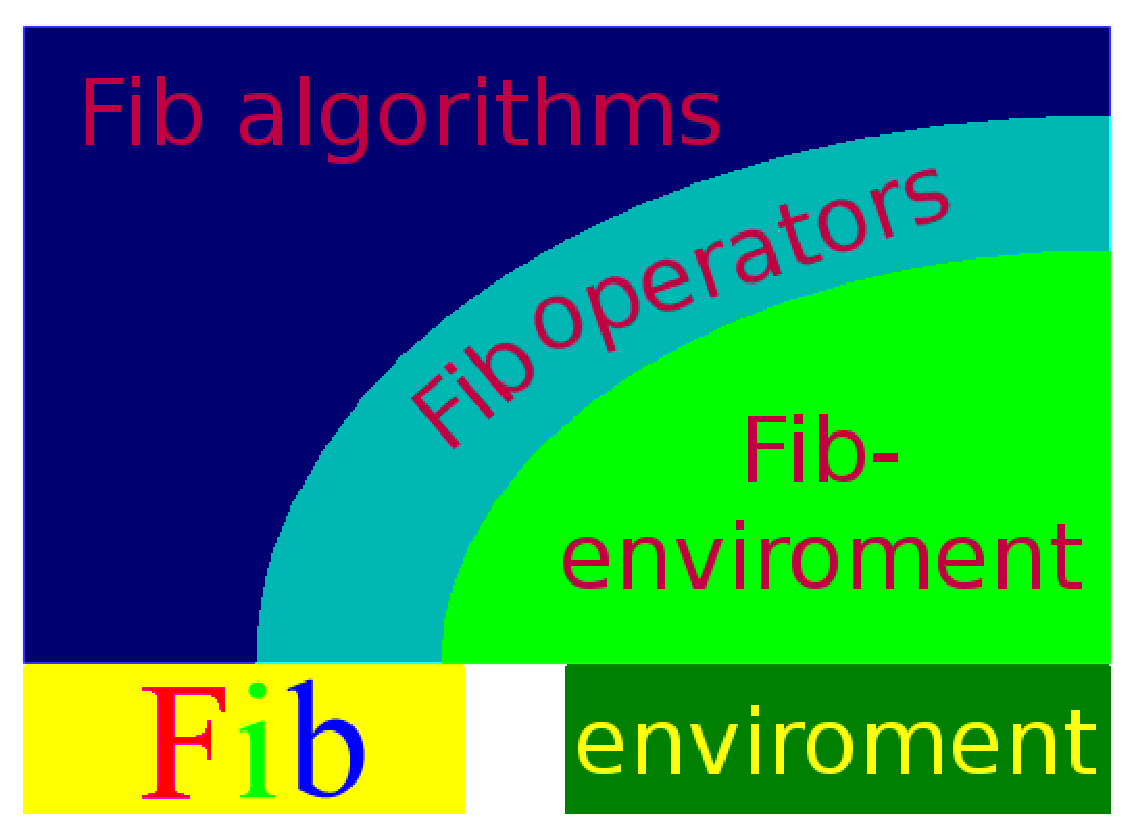
\includegraphics[scale=0.5]{project_dependencies}
\end{center}
\caption{Dependencies of the main modules}
\label{figMainModulDependencies}
\end{figure}

The ``enviroment.fib'' module requires for its individuals the Fib objects, but only as a name (for Fib objects). The ``enviroment.fib'' module thus only needs one name for Fib objects and no knowledge of the functionality (methods) of the Fib objects. Therefore the ``enviroment.fib'' module is not dependent on the ``fib'' module.

















%TODO references
%%\input{fib_sprachimplementation_en}%TODO 
%%\input{enviroment_implementation_en}%TODO
%%\input{fib_enviroment_implementation_en}%TODO
%%%
% Copyright (c) 2011  Betti "Osterholz
%
% Permission is granted to copy, distribute and/or modify this document
% under the terms of the GNU Free Documentation License, Version 1.2 or
% any later version published by the Free Software Foundation;
% with no Invariant Sections, no Front-Cover Texts, and no Back-Cover Texts.
%
% A copy of the license is included in the file ``fdl.tex'' .
%

%path for pictures
%\graphicspath{{./material_sprachbeschreibung/}}
%\graphicspath{{./material_sprachbeschreibung/}{../material_sprachbeschreibung}}


\newpage
\part{Fib-Datenbank}
\label{partFibDatabase}

Die Fib-Datenbank bietet die M"oglichkeit h"aufig verwendete Fib-Objekte vorzuhalten. Auf dort abgelegte Fib-Objekte kann von einem Fib-Multimediaobjekt zur"uckgegriffen werden, ohne dass diese mit dem Multimediaobjekt "ubertragen oder gespeichert werden m"ussen. Auf diese Weise kann nicht nur "Ubertragungsbandbreite 
gespaart werden, sondern mit dem Wissen "uber die festen Datenbankobjekte kann auch weitere Informationen aus dem Multimediaobjekt extrahiert werden.

Die Fib-Datenbank geh"ort zu keinem Fib-Multimediaobject. Sie wird mit den Fib-Bib\-lio\-the\-ken /dem Fib-System ausgeliefert und enth"alt h"aufig verwendete Datenbankobjekte, die in Fib-Objekten verwendet werden k"onnen. Datenbankobjekte k"onnen beispielsweise Linien (mit den Eingabeparametern f"ur Start- und Endpunkte), Recht\-ecke oder Kreise sein, aber auch B"aume, Autos, Zeichens"atze (fonts) oder Fraktale. Wird in einem Fib-Objekt beispielsweise ein Kreis ben"otigt, kann dass entsprechende parametrisierte Datenbankobjekt verwendet werden.

Die Implementierung der Datenbankobjekte kann an die jeweilige Anwendungsumgebung angepasst sein. Soll zur Anzeige beispielsweise OpenGL verwendet werden, k"onnen Datenbankobjekte direkt mit OpenGL-Primitiven (z. B. Dreiecken) umgesetzt werden. Auf diese Weise kann mit Datenbankobjekten die Performance der Anwendung verbessert werden. Bei der Kodierung der Fib-Objekte kann auch gleich darauf geachtet werden, dass Datenbankobjekte mit guter Performance f"ur die Zielanwendung verwendet werden. Diese Fib-Objekte sind dann immer noch auf allen Fib-Systemen mit gen"ugend hoher Datenbankversion anzeigbar, auf einigen jedoch schneller.

Welche Objekte eine Datenbank enth"alt, sowie die Identifier f"ur diese Objekte, sind mit der Datenbankversion festgelegt. Datenbanken mit h"oheren Datenbankversionen enthalten dabei alle Datenbankobjekte mit den gleichen Identifiern wie Datenbanken mit niedrigeren Datenbankversionen. Auf diese Weise ist gew"ahrleistet, dass Fib-Objekte immer aufw"artskompatibel zu neueren Datenbankversionen sind.

Alle Identifier von Datenbankobjekten sind negativ.


\section{Struktur}

Die Fib-Datenbank ist in verschiedene Abschnitte strukturiert.
Dabei sollten "ahnliche Objekte auch nahe beieinander stehen und wahrscheinlich h"aufig verwendete Objekte eine m"oglichst gro"se Identifier haben (also vom Absolutwert kleinen Identifier, da die Datenbankobjekidentifier alle negativ sind).

\bigskip\noindent
Die Beschreibung der einzelnen Bereiche (vorne stehen die Absolutwerte der Identifier (=Id), also 10 - 19 f"ur Id -10 bis -19):
\begin{itemize}
 \item 0 ein Objekt f"ur nichts (leerer Punkt)
 \item 1 - 9 Punkte (Id = Anzahl der Dimensionen)
 \item 10 - 19 Beschreibungen (wichtigste Lizenzen)
 \item 20 - 999 2 dimensionale Objekte:
 \begin{itemize}
  \item 20 - 29 Linien
  \item 30 - 39 Dreiecke
  \item 40 - 49 Vierecke
  \item 50 - 59 Kreise
  \item 60 - 89 offen
  \item 90 - 99 Funktionen
  \item 100 - 199 Beschreibungen 2 (z. B. Lizenzen)
  \item 200 - 299 Linien 2
  \item 300 - 399 Dreiecke 2
  \item 400 - 499 Vierecke 2
  \item 500 - 599 Kreise 2
  \item 600 - 899 offen
  \item 900 - 999 Funktionen 2
 \end{itemize}
 \item 1000 - 1999 Algorithmen
 \item 2000 - 2999 Beschreibungen
 \item 3000 - 3999 3 dimensionale Objekte
 \item 4000 - 4999 4 dimensionale Objekte

\end{itemize}


%TODO

%\section{Wichtige Datenbankobjekte}




%\section{Alle Datenbankobjekte}
















%TODO
%%\input{fib_konvertierungsfunktionen_en}%TODO
%%\input{fib_vorgehensweisen_en}%TODO
%%\input{fib_ergebnisse_en}%TODO
%%TODO: \input{fib_player_en}
%%\input{fib_algorithmen_en}%TODO
%%\input{fib_operatoren_en}%TODO

\newpage
\part{Appendix}

%\section{Implemtierungskonventionen}

%% Autor: Betti "Osterholz
% erstellt:5.11.2006
% Implementationskonverntionen V0.1
% Im Nachfolgendem sind einige Implementationskonverntionen aufgestellt
%
% Copyright (c) 2008 Betti "Osterholz
%
% Permission is granted to copy, distribute and/or modify this document
% under the terms of the GNU Free Documentation License, Version 1.2 or
% any later version published by the Free Software Foundation;
% with no Invariant Sections, no Front-Cover Texts, and no Back-Cover Texts.
%
% A copy of the license is included in the file ``fdl.tex'' .
%

\subsection{Allgemeines}

Zur Dokumentierung des Quelltextes wird \textbf{doxygen} im Java Stil verwendet.

Nur Kommentare die sich direkt auf spezifische Codeabschnitte beziehen erfolgen nicht im doxygen Stil.

Beim Quelltext wird gro"ser Wert auf Verst"andlichkeit und "Ubersichtlichkeit gelegt.
Die Sprache des Quelltexts (inclusive Quelltextkommentare ) ist Englisch.


\subsection{\index{Implementation!Einleitung}Einleitung des Quelltextes}

Jede Quelltextdatei beginnt mit einem Informationsheader beziehungsweise einer Dateieinleitung. In ihm steht der Name der Datei, des Autors und das Erstellungsdatum der Datei, gefolgt einer Kurzbeschreibung und den Kopierrechten(Copyright). Nach den Kopierrechten wird der Inhalt der Datei n"aher beschrieben.

Am Ende der Dateieinleitung folgt ein "Anderungsprotokoll, welches nicht in doxygen Stiel geschrieben wird.

\noindent
Beispiel:
\begin{verbatim}
/**
 * @class cDomains
 * file name: cDomains.cpp
 * @author Betti Oesterholz
 * @date 09.06.2009
 * @mail webmaster@BioKom.info
 *
 * System: C++
 *
 * This class represents a list of domains.
 * Copyright (C) @c LGPL3 2009 Betti Oesterholz
 *
 * This program is free software: you can redistribute
 * it and/or modify it under the terms of the
 * GNU Lesser General Public License (LGPL) as published
 * by the Free Software Foundation, either version 3 of
 * the License, or any later version.
 *
 * This program is distributed in the hope that it will
 * be useful, but WITHOUT ANY WARRANTY; without even
 * the implied warranty of MERCHANTABILITY or FITNESS
 * FOR A PARTICULAR PURPOSE. See the GNU Lesser General
 * Public License for more details.
 *
 * You should have received a copy of the GNU Lesser
 * General Public License along with this program.
 * If not, see <http://www.gnu.org/licenses/>.
 *
 *
 * This class represents a list of domains for an
 * root-element.
 * The domain list consists of a number of domains with
 * a type.
 *
 */
/*
History:
09.06.2009  Oesterholz  created
12.07.2009  Schmidt     new method to get the size of
   an domainelement
*/
\end{verbatim}

\subsection{\index{Implementation!Formatierung}Formatierung}

Gearbeitet wird mit Tabulatoren. Jeder Block, au"ser Methodenimplementationen und einzeilige Bl"ocke, wird durch ein Tab einger"uckt.

Die einzelenen Elemente in einer Zeile werden nach M"oglichkeit durch Leerzeichen seperiert. Die L"ange einer Zeile sollte m"oglichst 75 Zeichen nicht "uberschreiten.

\noindent
Beispiel:
\begin{verbatim}
if ( a == b ){
   //it makes something
   do_it;
   call( parameter );
}
\end{verbatim}

\subsection{\index{Implementation!Kommentare}Kommentare}

Alle Kommentare sind in Englisch gehalten.

Jede Methode beginnt mit einem Informationsheader im \textbf{doxygen} im Java Stil, in dem eine kurze Beschreibung der Methode steht.

Kommentare zu eine Quelltextsegment stehen in einer Zeile direkt vor diesem.


\subsection{\index{Implementation!Notation}Namen}

Namen sind Bezeichner von Klassen, Methoden, Variablen, Konstanten oder Makros.


\subsubsection{\index{Implementation!Notation!Klassennamen}\index{Notation!Klassennamen}Klassennamen}

Alle Klassennamen beginnen mit einem Kleinen "`c"' f"ur "`class"', die Teilworte des Klassennamen beginnen mit einem gro"sen Buchstaben
(Camelcase).

\noindent
Beispiel: cDomain; cDomainInteger

\subsubsection{\index{Implementation!Notation!Klassennamen besondere}\index{Notation!Klassennamen besondere}Namen f"ur besondere Klassentypen}
%TODO translate

F"ur einige Klassentypen gibt es bei der Bennenung f"ur den Anfangsbuchstagen Ausnahmen (sie beginnen dann nicht mit einem "`c"' f"ur "`class"').

\noindent
Die Anfangsbuchstagen f"ur die Klassentypen sind:
\begin{table}
	\centering
		\begin{tabular}{r|l}\hline
			K"urzel & Klassentyp\\\hline
			c & normale Klasse\\
			i & Interface\\
			l & Listener-Interface (Interface zum Empfangen von Events)\\
			e & Event-Klasse (enth"alten die Informationen f"ur Ereignisse)\\
		\end{tabular}
\caption{Prefixe f"ur Klassentypen}
\label{tabDatatypsPrefixe}
\end{table}

\noindent
Beispiel: iVariableUser; lFibObjectInfoChanged


\subsubsection{\index{Implementation!Notation!Methodennamen}\index{Notation!Methodennamen}Methodennamen}

Methoden beginnen mit einem Kleinbuchstaben. Teilnamen im Methodennamen beginnen mit einem gro"sen Buchstaben und grenzen unmittelbar aneinander. (Camelcase)

Methoden, die dazu dienen Werte zur"uckzugeben, beginnen mit einem "`get"'. Demgegen"uber beginnen Methoden, mit denen Werten gesetzt werden, sollen mit einem "`set"'.

\noindent
Beispiel:
\begin{itemize}
 \item eineMethod();
 \item getSomeThing();
\end{itemize}


\subsubsection{\index{Implementation!Notation!Variablennamen}\index{Notation!Variablennamen}Variablennamen}

Variablennamen beginnen kleingeschriebenen, Teilnamen im Variablennamen beginnen mit einem gro"sen Buchstaben und grenzen unmittelbar aneinander. (Camelcase) Namen von Variablen von grundlegenden Datentypen, wie Beispielsweise \texttt{int}, beginnen mit einem K"urzel f"ur diesen Datentypen (Siehe Tabelle \ref{tabDatatypsPrefixe}). Im Allgemeinen sollte am Variablennamenanfang der Typ der Variable erkennbar sein. Auch sollte der Variablennamen nach M"oglichkeit die Funktion der Variable beschreiben.

\begin{table}
	\centering
		\begin{tabular}{r|l}\hline
			K"urzel & Datentyp\\\hline
			i & int\\
			s & short\\
			c & char\\
			l & long\\
			u & unsigned\\
			p & pointer / Zeiger\\
			sz  & string / Zeichenketten\\
			li  & list / Listen\\
			vec & vector / Vektoren\\
			str & stream / Datenstrom\\
		\end{tabular}
\caption{Prefixe f"ur Variablennamen}
\label{tabDatatypsPrefixe}
\end{table}

\noindent
Beispiel: variableName, uiCounterDomain
%\subsubsection{\index{Implementation!Notation!Konstantennamen}\index{Notation!Konstantennamen}Konstantennamen}


%\subsubsection{\index{Implementation!Notation!Defines}\index{Implementation!Notation!Makros}\index{Notation!Defines}\index{Notation!Makros}Namen f"ur Makros}




%TODO

\input{gpl-3_0}
\input{lgpl-3_0}

\input{fdl}


\clearpage
\nocite{CI}\nocite{ECDF00}\nocite{ECTF}\nocite{LS}\nocite{UZ}\nocite{WT}\nocite{GADA}\nocite{GP}\nocite{EACD}\nocite{CTW}\nocite{CE}\nocite{GEA}\nocite{projBildf}\nocite{ESF}\nocite{GPFD}\nocite{AEFR}\nocite{Genocop}\nocite{HHGuideEC}\nocite{WOBC}\nocite{CMIT}\nocite{LDD_2007}\nocite{HKI2003}\nocite{CgBv2007}\nocite{VSys2003}\nocite{SEngPP2005}\nocite{CPPPR2004}\nocite{CC2004}\nocite{Russell2003}

%\bibliographystyle{gerplain}%deutscher bibliographie stiel
\bibliographystyle{amsplain}
\bibliography{literatur}

%TODO comment in
\index{multimedia information|see{root-element!multimedia information}}
\index{optional part|see{root-element!optional part}}
\index{domain|see{root-element!domain}}
%\index{Definitionsbereiche|see{cDomain}}
\index{subfunction|see{function element}}
\index{individual|see{cIndividual}}
%\index{cIndividual|see{Individuum}}
%\index{Kleiner Vergleich|see{cConditionLower}}


%\clearpage
%\part{Index}
\label{AbsIndex}
\printindex

\end{document}
